\graphicspath{{./figures/}}
\title{Optimization and OOO}
\date{}
\begin{document}
\usetikzlibrary{arrows.meta,chains,positioning,matrix,fit}


\ifdefined\NOBEAMER\else
\newcommand<>{\mathHL}[1]{%
\alt#2{
\text{\colorbox{green!20}{\ensuremath{#1}}}%
}{
\text{\colorbox{white!20}{\ensuremath{#1}}}%
}%
}
\fi

\makeatletter
\pgfdeclareshape{myregister}%
{
    \inheritsavedanchors[from=rectangle]
    \inheritanchorborder[from=rectangle]
    \inheritanchor[from=rectangle]{center}
    \inheritanchor[from=rectangle]{north}
    \inheritanchor[from=rectangle]{south}
    \inheritanchor[from=rectangle]{west}
    \inheritanchor[from=rectangle]{east}
    \inheritanchor[from=rectangle]{north east}
    \inheritanchor[from=rectangle]{north west}
    \inheritanchor[from=rectangle]{south east}
    \inheritanchor[from=rectangle]{south west}
    \inheritbackgroundpath[from=rectangle]
    \saveddimen{\halfbaselength}{%
         \pgf@x=0.5\wd\pgfnodeparttextbox
         % get xsep
         \pgfmathsetlength\pgf@xc{\pgfkeysvalueof{/pgf/inner xsep}}%
         \advance\pgf@x by \pgf@xc%
         % get \ht of textbox, add to baselength 
         \advance\pgf@x by \wd\pgfnodeparttextbox
         % get minimum width
         \pgfmathsetlength\pgf@xb{\pgfkeysvalueof{/pgf/minimum width}}%
         \divide\pgf@xb by 2
         \ifdim\pgf@x<\pgf@xb%
             % yes, too small. Enlarge...
             \pgf@x=\pgf@xb%
         \fi%
     }
    \backgroundpath{
        \pgfpathrectanglecorners{\southwest}{\northeast}
        \southwest \pgf@xa=\pgf@x \pgf@ya=\pgf@y 
        \pgf@yb=\pgf@ya
        \northeast \pgf@xb=\pgf@x %\pgf@yb=\pgf@y
        \pgf@xc = \pgf@xa
        \advance\pgf@xc by \halfbaselength
        \pgf@yc=\pgf@ya
        \advance\pgf@yc by \halfbaselength
        \pgfpathmoveto{\pgfpoint{\pgf@xa}{\pgf@ya}}
        \pgfpathlineto{\pgfpoint{\pgf@xc}{\pgf@yc}}
        \pgfpathlineto{\pgfpoint{\pgf@xb}{\pgf@yb}}
        \pgfpathclose
    }
}
\makeatother

\newcommand{\rA}{\it rA}
\newcommand{\rB}{\it rB}
\newcommand{\V}{\it V}
\newcommand{\D}{\it D}
\newcommand{\fn}{\it fn}
\newcommand{\Dest}{\it Dest}
\newcommand{\cc}{\it cc}
\tikzset{extra box/.style={},
         extra box opcode/.style={},
         extra box fn/.style={},
         extra box cc/.style={},
         extra box register/.style={},
         extra box immediate/.style={},
         extra box shorter width/.style={},
         extra box fake/.style={},
         }
\newcommand{\instrEncodingStyles}{
\tikzset{
    empty box/.style={text height=1ex,text depth=.4ex,font=\tt\fontsize{9}{10}\selectfont},
    box/.style={draw,rectangle,thick,empty box,extra box,align=center},
    opcode/.style={box,fill=blue!40!white,extra box opcode},
    secondOpcode/.style={box,fill=violet!40!white},
    secondOpcodeFN/.style={secondOpcode,extra box fn},
    secondOpcodeCC/.style={secondOpcode,extra box cc},
    literal/.style={box,fill=white!90!black},
    register/.style={box,fill=red!40!white,extra box register},
    fake/.style={empty box,pattern color=red!40!white,pattern=north west lines,inner sep=-1pt,extra box fake},
    immediate/.style={box,fill=green!40!white,extra box immediate},
    immediateLabel/.style={box,fill=green!40!white,extra box immediate,label={center:\fontsize{9}{10}\selectfont##1}},
}
}
\newcommand{\ccify}[2]{\begin{tikzpicture}[baseline]\node[anchor=base,secondOpcodeCC,text width=.35cm,inner xsep=0pt,inner sep=2pt,outer sep=0pt]{#1};\end{tikzpicture}}
\newcommand{\fnify}[1]{\begin{tikzpicture}[baseline]\node[anchor=base,secondOpcodeFN,text width=.35cm,inner xsep=0pt,inner sep=2pt,outer sep=0pt]{#1};\end{tikzpicture}}
\newcommand{\fnifyWide}[1]{\begin{tikzpicture}[baseline]\node[anchor=base,secondOpcodeFN,inner xsep=0pt,inner sep=2pt,outer sep=0pt,dashed]{#1};\end{tikzpicture}}
\newcommand{\opify}[1]{\begin{tikzpicture}[baseline]\node[anchor=base,opcode,text width=.35cm,inner xsep=0pt,inner sep=2pt,outer sep=0pt]{#1};\end{tikzpicture}}
\newcommand{\opifyWide}[1]{\begin{tikzpicture}[baseline]\node[anchor=base,opcode,inner xsep=0pt,inner sep=2pt,outer sep=0pt]{#1};\end{tikzpicture}}
\newcommand{\literalify}[1]{\begin{tikzpicture}[baseline]\node[anchor=base,literal,text width=.35cm,inner xsep=0pt,inner sep=2pt,outer sep=0pt]{#1};\end{tikzpicture}}
\newcommand{\immedify}[1]{\begin{tikzpicture}[baseline]\node[anchor=base,immediate,inner xsep=0pt,inner sep=2pt,outer sep=0pt]{#1};\end{tikzpicture}}
\newcommand{\rnify}[1]{\begin{tikzpicture}[baseline]\node[anchor=base,register,text width=.35cm,inner xsep=0pt,inner sep=2pt,outer sep=0pt]{#1};\end{tikzpicture}}
\newcommand{\rnifyWide}[1]{\begin{tikzpicture}[baseline]\node[anchor=base,register,inner xsep=0pt,inner sep=2pt,outer sep=0pt,dashed]{#1};\end{tikzpicture}}

\newcommand{\movq}{{\keywordstyle movq}\xspace}
\newcommand{\rmmovq}{{\keywordstyle rmmovq}\xspace}
\newcommand{\mrmovq}{{\keywordstyle mrmovq}\xspace}
\newcommand{\addq}{{\keywordstyle addq}\xspace}
\newcommand{\subq}{{\keywordstyle subq}\xspace}
\newcommand{\xorq}{{\keywordstyle xorq}\xspace}
\newcommand{\andq}{{\keywordstyle andq}\xspace}
\newcommand{\asmj}{{\keywordstyle jmp}\xspace}
\newcommand{\call}{{\keywordstyle call}\xspace}
\newcommand{\halt}{{\keywordstyle halt}\xspace}
\newcommand{\ret}{{\keywordstyle ret}\xspace}
\newcommand{\nop}{{\keywordstyle nop}\xspace}
\newcommand{\irmovq}{{\keywordstyle irmovq}\xspace}
\newcommand{\rrmovq}{{\keywordstyle rrmovq}\xspace}
\newcommand{\jmp}{{\keywordstyle jmp}\xspace}

\tikzset{
    hReg/.style={draw,myregister,minimum width=.4cm,minimum height=2cm,label={[font=\small,align=center]-90:#1}},
    hhReg/.style={draw,myregister,minimum width=.3cm,minimum height=5.5cm,label={[font=\small,align=center]-90:#1}},
    horizReg/.style={draw,myregister,rotate=-90,minimum width=.1cm,minimum height=1cm,label={[font=\small,align=center,fill=white]90:#1}},
    wReg/.style={draw,myregister,minimum width=2cm,minimum height=.4cm,label={[font=\small]-90:#1}},
    hRegSmall/.style={draw,myregister,minimum height=.6cm,minimum width=.2cm,label={[font=\small,inner sep=.5mm,align=center]-90:#1}},
    hRegT/.style={hRegSmall,minimum height=.4cm},
    mem/.style={draw,rectangle,minimum height=1.5cm,minimum width=1cm,inner sep=4pt,align=center,font=\small},
    memBig/.style={draw,rectangle,minimum height=3cm,minimum width=3cm,align=center,font=\small},
    regFile/.style={draw,rectangle,minimum height=4cm,minimum width=2cm,align=center,font=\small},
    ll/.style={font=\scriptsize},
    a/.style={-{Latex[length=5pt,width=3pt]},thick},
    aR/.style={{Latex[length=5pt,width=3pt]}-,thick},
    aN/.style={thick},
    aa/.style={-{Latex[length=5pt,width=3pt]},line width=1.2pt},
    aaR/.style={{Latex[length=5pt,width=3pt]}-,line width=1.2pt},
    aaN/.style={line width=1.2pt},
    b/.style={-{Latex[length=2pt,width=2pt]}},
    bN/.style={thin},
    bb/.style={line width=.5pt,-{Latex[length=2pt,width=2pt]}},
    bbR/.style={line width=.5pt,{Latex[length=2pt,width=2pt]}-},
    bR/.style={{Latex[length=2pt,width=2pt]}-},
    global scale/.style={scale=#1,every node/.style={scale=#1}},
    %logicBlock/.style={draw,cloud,cloud puffs=13.7,inner sep=0pt,cloud ignores aspect,align=center,draw},
    logicBlock/.style={draw,rectangle,inner sep=1pt,align=center,draw,fill=blue!20},
    logicBlockS/.style={draw,rectangle,inner sep=1pt,align=center,draw,fill=blue!20,font=\small},
    control/.style={dashed,color=blue!60},
    logicFill/.style={fill=blue!20},
    offsetBox/.style={align=left,font=\small,draw=blue!60!black,line width=2pt,rectangle}
}

\tikzset{
    bookLabel/.style={color=red!60!black,font=\small\bfseries,outer sep=0pt,inner sep=1pt,fill=white},
    imemPcPre/.style={invisible},
    imemPc/.style={},
    instrRegs/.style={},
    instrRegsPre/.style={invisible},
    instrRegsSplitOut/.style={invisible},
    instrRegsSplitImmed/.style={instrRegsSplitOut},
    instrRegsRS1/.style={instrRegs},
    instrRegsMux/.style={instrRegs},
    instrRegsMuxRS2/.style={instrRegsMux},
    instrRegsMuxRS3/.style={instrRegsMux},
    instrRegsMuxRS3F/.style={instrRegsMuxRS3},
    instrRegsMuxRS4/.style={instrRegsMux},
    instrRegsRS34Loop/.style={invisible},
    instrRegsNoMux/.style={invisible},
    instrRegsNoMuxRS2/.style={instrRegsNoMux},
    instrRegsNoMuxRS3/.style={instrRegsNoMux},
    instrRegsNoMuxRS4/.style={instrRegsNoMux},
    instrRegsPreSingle/.style={invisible},
    regsLogic/.style={},
    regsLogicMux/.style={regsLogic},
    regsLogicMuxA/.style={regsLogicMux},
    regsLogicMuxB/.style={regsLogicMux},
    regsLogicNoMux/.style={invisible},
    regsLogicNoMuxA/.style={regsLogicNoMux},
    regsLogicNoMuxB/.style={regsLogicNoMux},
    logicDmem/.style={},
    logicDmemMux/.style={logicDmem},
    logicDmemNoMux/.style={invisible},
    dmemWB/.style={},
    dmemWBFromMem/.style={dmemWB},
    dmemWBvalENoMux/.style={dmemWB},
    dmemWBvalELoop/.style={invisible},
    dmemWBvalEMux/.style={invisible},
    dmemOutToPC/.style={dmemWB},
    dmemPC/.style={},
    dmemPCMux/.style={dmemPC},
    dmemPCNoMux/.style={invisible},
    pcDecode/.style={},
    isStatReg/.style={hRegSmall=#1},
    isStat/.style={invisible},
    dmemNorm/.style={},
    dmemInputLabel/.style={dmemNorm},
    dmemLabel/.style={invisible},
    dmemPre/.style={invisible},
    dmemPreSingle/.style={invisible},
    regNorm/.style={},
    regNormLabel/.style={},
    regNormLabelE/.style={regNormLabel},
    regNormLabelM/.style={regNormLabel},
    regPre/.style={},
    regPreSingle/.style={},
    ccsNorm/.style={invisible},
    smallLabel/.style={font=\scriptsize,inner sep=1pt,outer sep=0pt},
    smallerLabel/.style={font=\tiny,inner sep=1pt,outer sep=0pt},
    pcStyle/.style={},
    wbPCLine/.style={},
    aluOpExplain/.style={regsLogic},
    funcOpExplain/.style={logicDmem},
    muxDst/.style={},
}
\newcommand{\instrEncodingSubTable}[3]{
\matrix[matrix of nodes,
    column sep=-2\pgflinewidth,
    row sep=2.5pt,
    nodes={empty box,text width=.35cm,inner xsep=0pt, inner sep=2pt,outer sep=0pt},
    column 1/.style={nodes={font=\tt\fontsize{9}{10}\selectfont,text width=3.5cm}},
    column 6/.style={nodes={extra box shorter width}},
    column 7/.style={nodes={extra box shorter width}},
    column 8/.style={nodes={extra box shorter width}},
    column 9/.style={nodes={extra box shorter width}},
    column 10/.style={nodes={extra box shorter width}},
    column 11/.style={nodes={extra box shorter width}},
    column 12/.style={nodes={extra box shorter width}},
    column 13/.style={nodes={extra box shorter width}},
    column 14/.style={nodes={extra box shorter width}},
    column 15/.style={nodes={text width=.2cm,extra box shorter width}},
    column 16/.style={nodes={text width=.2cm,extra box shorter width}},
    column 17/.style={nodes={text width=.2cm,extra box shorter width}},
    column 18/.style={nodes={text width=.2cm,extra box shorter width}},
    column 19/.style={nodes={text width=.2cm,extra box shorter width}},
    column 20/.style={nodes={text width=.2cm,extra box shorter width}},
    column 21/.style={nodes={text width=.2cm,extra box shorter width}},
#1,
] (#2) {#3}}

\newcommand{\var}[1]{\ensuremath{\text{#1}}}
\newcommand{\icode}{\var{icode}}
\newcommand{\ifun}{\var{ifun}}
\newcommand{\vrA}{\var{rA}}
\newcommand{\vrB}{\var{rB}}
\newcommand{\valP}{\var{valP}}
\newcommand{\valA}{\var{valA}}
\newcommand{\valB}{\var{valB}}
\newcommand{\valC}{\var{valC}}
\newcommand{\valE}{\var{valE}}
\newcommand{\valM}{\var{valM}}
\newcommand{\PC}{\var{PC}}
\newcommand{\srcA}{\var{srcA}}
\newcommand{\srcB}{\var{srcB}}
\newcommand{\dstE}{\var{dstE}}
\newcommand{\dstM}{\var{dstM}}
\newcommand{\aluA}{\var{aluA}}
\newcommand{\aluB}{\var{aluB}}
\newcommand{\pcMemDist}{2.cm}
\newcommand{\imemRegsDist}{3.5cm}
\newcommand{\regAluDist}{1.25cm}
\newcommand{\regMemDist}{3cm}
\newcommand{\regMuxDmemDist}{1.5cm}
\newcommand{\regReadOffset}{0cm}
\newcommand{\dstMuxDelta}{2.5mm}
\newcommand{\ilenOffset}{0cm}
\newcommand{\pcLabel}{PC}
\newcommand{\prePcDist}{2.5mm}
\newcommand{\regRegLabelDist}{1.5cm}
\newcommand{\regBDist}{.4cm}

\newcommand{\circuitStateToALU}{
        \node[hReg=\pcLabel,pcStyle] (pc) {};
        \node[mem,right=\pcMemDist of pc,font=\scriptsize] (imem) {Instr. \\ Mem.};
        \coordinate (imemData) at (imem.east);
        \coordinate (imemAddr) at (imem.west);
        \begin{scope}[regNorm]
            \node[regFile,right=\imemRegsDist of imem,label={[label distance=1pt,inner sep=0pt]\small register file}] (regs) {};
            \coordinate (regSelect1) at ($(regs.north west) - (0cm, .5cm)$);
            \coordinate (regSelect2) at ($(regs.north west) - (0cm, 1cm)$);
            \coordinate (regSelect3) at ($(regs.north west) - (0cm, 1.5cm)$);
            \coordinate (regSelect4) at ($(regs.north west) - (0cm, 2cm)$);
            \coordinate (regWriteIn1) at ($(regs.north west) - (0cm, 3.0cm)$);
            \coordinate (regWriteIn2) at ($(regs.north west) - (0cm, 3.5cm)$);
            \coordinate (regRead1) at ($(regs.north east) - (0cm, .4cm)$);
            \coordinate (regRead2) at ($(regs.north east) - (0cm, .4cm) - (0cm, \regBDist)$);
            %\node[ll,below left=0pt of regWriteIn,outer sep=1pt,inner sep=0pt] {data};
        \end{scope}
        \begin{scope}[regNormLabel]
            \node[smallLabel,right=0mm of regSelect1] (srcALabel) {\srcA};
            \node[smallLabel,right=0mm of regSelect2] (srcBLabel) {\srcB};
            \node[smallLabel,left=0mm of regRead1] {R[\srcA]};
            \node[smallLabel,left=0mm of regRead2] {R[\srcB]};
        \end{scope}[regNormLabel]

        \begin{scope}[regNormLabelE]
            \node[smallLabel,right=0mm of regSelect4] (dstELabel) {\dstE};
            \node[smallLabel,right=0mm of regWriteIn2] {next R[\dstE]};
        \end{scope}
        \begin{scope}[regNormLabelM]
            \node[smallLabel,right=0mm of regSelect3] (dstMLabel) {\dstM};
            \node[smallLabel,right=0mm of regWriteIn1] {next R[\dstM]};
        \end{scope}
}

\newcommand{\circuitState}{
        \circuitStateToALU
        \begin{scope}[dmemNorm]
            \node[mem,right=\regMemDist of regs,minimum width=1.3cm] (dmem) {};
            \node[dmemLabel,align=center] at (dmem) {Data\\Mem.};
            \coordinate (dmemIn) at (dmem.west);
            \coordinate (dmemInHigh) at ([yshift=.3cm]dmem.west);
            \coordinate (dmemInLow) at ([yshift=-.3cm]dmem.west);
            \coordinate (dmemDataOut) at (dmem.east);
        \end{scope}
        \begin{scope}[ccsNorm]
            \node[below=1cm of dmem,hRegSmall=ZF/SF] (ccs) {};
        \end{scope}
        \begin{scope}[isStat]
            \node[isStatReg=Stat,below=.25cm of dmem] (Stat) {};
        \end{scope}
}
\newcommand{\circuitStatePre}{
        \begin{scope}[imemPcPre]
            \draw[thick,latex-] (pc.west) -- +(-.5cm,0cm);
            \draw[thick,latex-] (imemAddr) -- +(-.3cm,0cm);
            \draw[thick,-latex] (pc.east) -- +(.3cm,0cm);
            \draw[thick,-latex] (imemData) -- +(.5cm,0cm);
        \end{scope}
        \begin{scope}[regPre]
            \draw[a,-latex,double] (regRead1) -- +(.5cm,0cm);
            \draw[thick,double,latex-] (regWriteIn1) -- +(-.5cm,0cm);
        \end{scope}
        \begin{scope}[regPreSingle]
            \draw[a,-latex] (regRead1) -- +(.5cm,0cm);
            \draw[thick,latex-] (regWriteIn1) -- +(-.5cm,0cm);
            \draw[a,-latex] (regRead2) -- +(.5cm,0cm);
            \draw[thick,latex-] (regWriteIn2) -- +(-.5cm,0cm);
        \end{scope}
        \begin{scope}[instrRegsPre]
            %\foreach \x in {regSelect1,regSelect2} {
            %    \draw[latex-] (\x) -- +(-.5cm,0cm);
            %}
            \draw[b,latex-,double] (regSelect1) -- +(-.5cm,0cm);
        \end{scope}
        \begin{scope}[instrRegsPreSingle]
            \foreach \x in {regSelect1,regSelect2,regSelect3,regSelect4} {
                \draw[latex-] (\x) -- +(-.5cm,0cm);
            }
        \end{scope}
        \begin{scope}[dmemPre]
            \draw[thick,-latex] (dmemDataOut) -- +(.5cm,0cm);
            \draw[thick,double,latex-] (dmemIn) -- +(-.5cm,0cm);
        \end{scope}
        \begin{scope}[dmemPreSingle]
            \draw[thick,-latex] (dmemDataOut) -- +(.5cm,0cm);
            \draw[thick,latex-] (dmemInHigh) -- +(-.5cm,0cm);
            \draw[thick,latex-] (dmemInLow) -- +(-.5cm,0cm);
        \end{scope}
}
\newcommand{\dmemInput}{
    \begin{scope}[dmemInputLabel]
        \node[smallLabel,right=0mm of dmemInHigh] {Data in};
        \node[smallLabel,right=0mm of dmemInLow] {Addr in};
        \node[smallLabel,left=0mm of dmemDataOut] {Data out};
    \end{scope}
}

\newcommand{\circuitConnectDetail}{
    \dmemInput

    % PC/IMEM
    \begin{scope}[imemPc]
        \draw[a] (pc.east) -- (imemAddr);
    \end{scope}

    % IMEM/REGISTERS
    \begin{scope}[instrRegs]
        \coordinate (split) at ([xshift=1cm]imemData);
        \coordinate (splitIcode) at ([xshift=.15cm]imemData);
        \coordinate (splitImmed) at ([xshift=.25cm]imemData);
        \coordinate (splitrA) at ([xshift=.5cm]imemData);
        \coordinate (splitrB) at ([xshift=.75cm]imemData);
        \draw[line width=1.5pt] (imemData) -- (splitIcode);
        \draw[line width=1.25pt] (imemData) -- (splitImmed);
        \coordinate (aboveRegFile) at ([yshift=.5cm]regs.north);
        \coordinate (furtherAboveRegFile) at ([yshift=.75cm]regs.north);

        \begin{scope}[instrRegsSplitOut]
            \draw[b] (splitrA) |- ([xshift=-1cm]regSelect1);
            \draw[b] (splitrB) |- ([xshift=-1cm]regSelect2);
        \end{scope}
        \begin{scope}[instrRegsSplitImmed]
            \draw[a] (splitImmed) |- (aboveRegFile) node[right,bookLabel] {valC};
        \end{scope}

        \begin{scope}[instrRegsRS1]
            \draw[b] (splitrA) |- (regSelect1);
        \end{scope}

        \begin{scope}[instrRegsNoMuxRS2]
           \draw[b] (splitrB) |- (regSelect2);
        \end{scope}
        \begin{scope}[instrRegsNoMuxRS3]
            \draw[b] (splitrA) |- (regSelect3);
        \end{scope}
        \begin{scope}[instrRegsNoMuxRS4]
            \draw[b] (splitrB) |- (regSelect4);
        \end{scope}

        \draw[line width=.75pt] (imemData) -- (splitrA);
        \draw[line width=0.5pt] (splitrA) -- (splitrB);
        
            \begin{scope}[instrRegsMuxRS3]
                \node[draw,minimum height=2cm,minimum width=1.25cm,left=\dstMuxDelta of regSelect3,mux,inputs={nn},global scale=0.25] (muxDstM) {};
                \draw[thin] (splitrA |- muxDstM.input 1) -- ([xshift=-2pt]splitrB |- muxDstM.input 1);
                \draw[b] ([xshift=2pt]splitrB |- muxDstM.input 1) -- (muxDstM.input 1);
                \draw[b] (muxDstM.output) -- (regSelect3);
                %\draw[bR] (muxDstM.input 3) -| (splitrB);
            \end{scope}
            \begin{scope}[instrRegsMuxRS3F]
                \draw[bR] (muxDstM.input 2) -- ++(180:2.5mm) node[left,inner sep=0pt,font=\tiny\tt] {0xF};
            \end{scope}
            \begin{scope}[instrRegsMuxRS4]
                \node[draw,minimum height=2cm,minimum width=1.25cm,left=\dstMuxDelta of regSelect4,mux,inputs={nnn},global scale=0.25] (muxDstE) {};
                \draw[b] (muxDstE.output) -- (regSelect4);
                \draw[bR] (muxDstE.input 2) -- ++(180:2.5mm) node[left,inner sep=0pt,font=\tiny\tt] {0xF};

                \draw[b] (splitrB) |- (muxDstE.input 1);
                \draw[bR] (muxDstE.input 3) -- ++(-.25cm,-.4mm) node[left,font=\tiny\tt,inner sep=0pt] {\%rsp};
            \end{scope}

            \begin{scope}[instrRegsMuxRS2]
                \node[draw,mux,minimum height=1.5cm,minimum width=0.5cm,global scale=0.25,inputs={nn},anchor=output,minimum height=1cm] (muxSrcB) at ([xshift=-.25cm]regSelect2) {};

                \draw[b] (muxSrcB.output) -- (regSelect2);
                \draw[b] (splitrB) |- (muxSrcB.input 1);
                \draw[bR] (muxSrcB.input 2) -- ++(-.25cm,-.25mm) node[left,font=\tiny\tt,inner sep=0pt] {\%rsp};
            \end{scope}

            \begin{scope}[instrRegsRS34Loop]
                \node[draw,minimum height=2cm,minimum width=1cm,mux,inputs={nnn},global scale=0.25,muxDst] (muxDstEAbove)
                    at ([yshift=1cm]regs.north) {};
                \node[draw,minimum height=2cm,minimum width=1cm,mux,inputs={nn},global scale=0.25,muxDst] (muxDstMAbove)
                    at ([yshift=1.5cm]regs.north) {};

                \coordinate (splitOffRBLoop) at ([xshift=-1cm]regSelect2 |- muxSrcB.input 1);
                \draw[bN] ([xshift=-1.25cm]regSelect1) |- ([xshift=-1.25cm,yshift=-2pt]regSelect1 |- aboveRegFile);
                \draw[b] ([xshift=-1.25cm,yshift=2pt]regSelect1 |- aboveRegFile) |- (muxDstMAbove.input 2);
                \draw[bN] (splitOffRBLoop) -- ([yshift=-2pt]splitOffRBLoop |- regSelect1);
                \draw[bN] ([yshift=2pt]splitOffRBLoop |- regSelect1) -- ([yshift=-2pt]splitOffRBLoop |- aboveRegFile);
                %\draw[b] ([yshift=2pt]splitOffRBLoop |- aboveRegFile) |- (muxDstMAbove.input 3);
                \draw[bR] (muxDstMAbove.input 1) -- ++(180:2.5mm) node[left,inner sep=0pt,font=\tiny\tt] {0xF};

                \draw[bR] (muxDstEAbove.input 1) -- ++(180:2.5mm) node[left,inner sep=0pt,font=\tiny\tt] {0xF};
                \draw[bR] (muxDstEAbove.input 2) -- ++(180:2.5mm) node[left,inner sep=0pt,font=\tiny\tt] {\%rsp};
                \draw[b] ([yshift=2pt]splitOffRBLoop |- aboveRegFile) |- (muxDstEAbove.input 3);

                \coordinate (dstMUpperRightCorner) at ([xshift=.5cm,yshift=2cm]dmem.north east);
                \coordinate (dstEUpperRightCorner) at ([xshift=.4cm,yshift=1.9cm]dmem.north east);
                \coordinate (dstMLowerRightCorner) at ([xshift=.5cm,yshift=-2.3cm]dmem.south east);
                \coordinate (dstELowerRightCorner) at ([xshift=.4cm,yshift=-2.2cm]dmem.south east);
                \coordinate (dstELeft) at ([xshift=-.75cm]regs.west);
                \coordinate (dstMLeft) at ([xshift=-1cm]regs.west);
                \coordinate (badLineHeight) at ([yshift=-.75cm]regs.south west);
                \draw[bN] (muxDstMAbove.output) -- ++(0.35cm, 0cm) |- (dstMUpperRightCorner) -- (dstMLowerRightCorner)
                    -| ([yshift=-2pt]dstMLeft |- badLineHeight);
                \draw[b] ([yshift=2pt]dstMLeft |- badLineHeight) |- (regSelect3);
                \draw[bN] (muxDstEAbove.output) -- ++(0.25cm, 0cm) |- (dstEUpperRightCorner) -- (dstELowerRightCorner)
                    -| ([yshift=-2pt]dstELeft |- badLineHeight);
                \draw[b] ([yshift=2pt]dstELeft |- badLineHeight) |- (regSelect4);
            \end{scope}
        
        \node[left=\regRegLabelDist of regSelect1,fill=white,font=\tiny,inner sep=1pt,outer sep=0pt] (vrALabel) {\vrA};
        \node[left=\regRegLabelDist of regSelect2,fill=white,font=\tiny,outer sep=0pt,inner sep=1pt] (vrBLabel) {\vrB};
    \end{scope}


    % REGISTERS/ALU
    % + ALU component
    \begin{scope}[regsLogic]
        \node[right=\regAluDist of regs,minimum height=1cm,minimum width=.75cm,logicBlock,label={[label distance=1pt,inner sep=0pt]\small ALU}] (alu) {};
        \coordinate (aluTop) at ([yshift=-2mm]alu.north west);
        \coordinate (aluBottom) at ([yshift=2mm]alu.south west);
        \node[smallerLabel,right=0mm of aluTop] {\aluA};
        \node[smallerLabel,right=0mm of aluBottom] {\aluB};
        \node[smallerLabel,left=0mm of alu.east] {\valE};
        \coordinate (afterAlu) at ([xshift=1mm]alu.east);

        \coordinate (regReadAfter1Pre) at ([xshift=4mm]regRead1);
        \coordinate (regReadAfter1) at ([xshift=\regReadOffset]regReadAfter1Pre);
        \coordinate (regReadAfter2Pre) at ([xshift=1mm]regRead2);
        \coordinate (regReadAfter2) at ([xshift=\regReadOffset]regReadAfter2Pre);
        
        \begin{scope}[regsLogicMuxA]
            \node[draw,mux,global scale=0.45,minimum height=1cm,left=2.5mm of aluTop,inputs={nnn}] (muxAluA) {};
            \draw[a] (muxAluA.output) -- (aluTop);
            \draw[a] (regRead1) -- (regReadAfter1) |- (muxAluA.input 2);
            \coordinate (dmemInBefore) at ([xshift=-2.5mm]dmemInHigh);
            \coordinate (beforeMux1) at ([xshift=-2.5mm]muxAluA.input 1);
            \coordinate (immedPreAlu) at ([xshift=-2.5mm,yshift=4pt] regRead1 -| muxAluA.input 1);
            \draw[aN] (splitImmed) |- (aboveRegFile) -| (immedPreAlu);
            \draw[a] ([xshift=-2.5mm,yshift=-4pt] regRead1 -| muxAluA.input 1) |- (muxAluA.input 1);
            \draw[bR] (muxAluA.input 3) -- ++(-.1cm,-.2cm) node[left,font=\tiny\tt,inner sep=0pt] {8};
        \end{scope}

        \begin{scope}[regsLogicMuxB]
            \node[draw,mux,minimum height=1.5cm,minimum width=.5cm,global scale=0.35,inputs={nn},anchor=output] (muxAluB) at ([xshift=-.5cm]aluBottom) {};
            \draw[a] (regRead2) -- (regReadAfter2) |- (muxAluB.input 1);
            \draw[aR] (muxAluB.input 2) -- ++(-.25cm,0cm) node[left,font=\tiny\tt,inner sep=0pt]{0};
            \draw[a] (muxAluB.output) -- (aluBottom);
        \end{scope}

        \begin{scope}[regsLogicNoMuxB]
            \draw[a] (regRead2) -- (regReadAfter2) |- (aluBottom);
        \end{scope}
        \begin{scope}[regsLogicNoMuxA]
            \draw[a] (regRead1) -- (regReadAfter1) |- (aluTop);
        \end{scope}

        % ALU Registers
        \draw[bR,aluOpExplain] (alu.south) -- ++(0,-2.5mm) node[below,inner sep=0pt,align=center,font=\tiny,aluOpExplain] (aluOpExplain) {add/sub\\ xor/and \\ (function \\ of instr.)};
    \end{scope}

    \begin{scope}[dmemPC]
        \node[dmemPCMux,draw,minimum height=2cm,left=.25cm of pc,mux,inputs={nnn},global scale=0.5] (muxPc) {};
    \end{scope}


    % ALU/MEMORY
    \begin{scope}[logicDmem]
        \node[smallerLabel,above=0mm of dmem.south] {write?};
        
        \draw[bR,funcOpExplain] (dmem.south) -- ++(0,-2.5mm) node[funcOpExplain,below,align=center,inner sep=0pt,font=\tiny] (funcOpExplain) {function\\of opcode};

        % MEMORY Registers
            % FIXME: correct input?
        \begin{scope}[logicDmemMux]
            \node[draw,mux,minimum height=1cm,global scale=0.45,left=5mm of dmemInLow,inputs={nn}] (muxDAddr) {};
            \draw[a] (muxDAddr.output) -- (dmemInLow);
            \draw[a] (regRead2) -- (regReadAfter2) |- ([yshift=-1mm,xshift=.5mm]alu.south east) |- (muxDAddr.input 2);
            \draw[a] (alu.east) -- (afterAlu) |- (muxDAddr.input 1);

            \node[draw,mux,minimum height=1cm,global scale=0.5,inputs={nn},anchor=input 2,minimum height=1cm] (muxDMem) at ([xshift=\regMuxDmemDist]regRead1) {};
            \draw[a] (muxDMem.output) -| (dmemInBefore) -- (dmemInHigh);
            \draw[a] (regRead1) -- (muxDMem.input 2);
            \coordinate (immedIntersect) at ([xshift=.5cm,yshift=2.5mm]pc.north east);
            %\draw[aN] (pc.east) -| ([yshift=-4pt]immedIntersect); 
            %\draw[a] ([yshift=4pt]immedIntersect) |- (furtherAboveRegFile) -| ([xshift=-2.5mm]muxDMem.input 1)
            %            -- (muxDMem.input 1);
            \draw[aR] (muxDMem.input 1) -- ++ (-.25cm, 0cm) -- ++ (0cm, .25cm) node[above,font=\scriptsize,inner sep=0.5mm] {PC+9};
        \end{scope}

        \begin{scope}[logicDmemNoMux]
            \draw[a] (alu.east) -- (afterAlu) |- (dmemInLow);
            \draw[a] (regRead1) -| ([xshift=-.5cm]dmemInHigh) -- (dmemInHigh);
        \end{scope}
    \end{scope}
    
    \begin{scope}[dmemWBvalENoMux]
        \draw[aN] (alu.east) -- (afterAlu) -- ([yshift=.025cm]afterAlu |- muxDAddr.input 2);
        \draw[a] ([yshift=-.025cm]afterAlu |- muxDAddr.input 2) |- ([yshift=-.25cm,xshift=-.25cm]regs.south west) |- (regWriteIn2);
    \end{scope}
    \begin{scope}[dmemWBvalELoop]
        \draw[aN] (alu.east) -- (afterAlu) -- ([yshift=.025cm]afterAlu |- muxDAddr.input 2);
        \draw[a] ([yshift=-.025cm]afterAlu |- muxDAddr.input 2) |- ([yshift=-.15cm]dmem.south west) |- ([yshift=-.25cm,xshift=-.25cm]regs.south west) |- (regWriteIn2);
    \end{scope}
    \begin{scope}[dmemWBvalEMux]
        \node[draw,mux,minimum height=1cm,global scale=0.5,inputs={nnn},rotate=180] (muxValE) at ([yshift=-.25cm, xshift=.1cm]regs.south east) {};
        \draw[a] (alu.east) -- (afterAlu) |- (muxValE.input 3);
        \draw[aN] (regRead1) -- (regReadAfter1) -- ([yshift=.05cm]regReadAfter1 |- aluBottom);
        \draw[aN] ([yshift=-.05cm]regReadAfter1 |- aluBottom) -- ([yshift=-.05cm]regReadAfter1 |- alu.south);
        \draw[a] ([yshift=-.15cm]regReadAfter1 |- alu.south) |- (muxValE.input 1);
        \draw[a] (muxValE.output) -- ([yshift=-.25cm,xshift=-.25cm]regs.south west) |- (regWriteIn2);
        \draw[aN] ([yshift=1cm]immedPreAlu) -- ([yshift=.05cm]immedPreAlu |- muxAluA.input 2);
        \draw[aN] ([yshift=-.05cm] immedPreAlu |- muxAluA.input 2) -- ([yshift=.05cm]immedPreAlu |- aluBottom);
        \draw[a] ([yshift=-.05cm] immedPreAlu |- aluBottom) |- (muxValE.input 2);
    \end{scope}
    \begin{scope}[dmemWB]
        \draw[a] (dmemDataOut) -- ++(2.5mm,0) |- ([yshift=-.5cm,xshift=-.5cm]regs.south west) |- (regWriteIn1);
    \end{scope}
    \begin{scope}[dmemOutToPC]
        \draw[a] (dmemDataOut) -- ++(2.5mm,0) |- ([yshift=-.5cm,xshift=-.5cm]regs.south west) --
            ++ (0cm,-.25cm) -| ([xshift=-3.5mm]muxPc.input 2) -- (muxPc.input 2);
    \end{scope}

    % PC update mux
    \begin{scope}[dmemPC]
        % above: \node[left=.25cm of pc,mux,inputs={nnn},global scale=0.5] (muxPc) {};
        \node[xshift=\ilenOffset,below=1cm of imem,logicBlock,font=\small] (iLen) {instr.\\length};
        \node[left=.25cm of iLen,logicBlock,font=\small] (iLenPlus) {+};
        
        \draw[b] ([xshift=\ilenOffset]splitIcode) |- (iLen.east);
        \draw[b] (iLen.west) -- (iLenPlus.east);
        \draw[a] (pc.east) -| (iLenPlus.north);

        \begin{scope}[dmemPCMux]
            \draw[a] (iLenPlus.west) -| ([xshift=-2.5mm]muxPc.input 3) -- (muxPc.input 3);

            \draw[a] (splitImmed) |- ([yshift=2.5mm]pc.north) -| ([xshift=-2.5mm]muxPc.input 1) -- (muxPc.input 1);

            \draw[a] (muxPc.output) -- (pc.west);
        \end{scope}
        
        \begin{scope}[dmemPCNoMux]
            \draw[a] (iLenPlus.west) -| ([xshift=-\prePcDist]pc.west) -- (pc.west);
        \end{scope}
    \end{scope}
    
}

\newcommand{\circuitConnect}{
        \begin{scope}[imemPc]
            \draw[a] (pc.east) -- (imemAddr);
        \end{scope}
        \begin{scope}[instrRegs]
            \node[logicBlock,right=1cm of imem,minimum height=6cm,minimum width=1cm] (decode) {logic};
            \draw[a] (imemData) -- (decode);
            \draw[b] (decode.east |- regSelect1) -- (regSelect1);
            \draw[b] (decode.east |- regSelect2) -- (regSelect2);
            \draw[b] (decode.east |- regSelect3) -- (regSelect3);
            \draw[b] (decode.east |- regSelect4) -- (regSelect4);
        \end{scope}
        \begin{scope}[regsLogic]
            \node[logicBlock,right=1cm of regs,minimum height=5.5cm,yshift=.25cm,minimum width=.1cm] (execute) {logic \\ (with\\ ALU)};
            \draw[a] (regRead1) -- (execute.west |- regRead1);
            \draw[a] (regRead2) -- (execute.west |- regRead2);
            \begin{scope}[ccsNorm]
                \draw[b] (ccs.east) -- (execute.west |- ccs.east);
            \end{scope}
        \end{scope}
        \begin{scope}[logicDmem]
            \draw[a, double] (execute.east |- dmemIn) -- (dmemIn);
            \draw[b,isStat] (execute.east |- Stat.west) -- (Stat.west);
            \coordinate (leftBelowExecute) at ($(execute.south east) + (.5cm,-.4cm)$);
            \coordinate (leftBelowExecute2) at ($(execute.south east) + (.75cm,-.5cm)$);
            \coordinate (leftBelowExecute3) at ($(execute.south east) + (.1cm,-.6cm)$);
            \coordinate (rightBelowExecute) at ($(execute.south east) + (-3cm,-.6cm)$);
            \coordinate (beforeReg1) at ($(regWriteIn1) + (-.125cm,0cm)$);
            \coordinate (beforeReg2) at ($(regWriteIn2) + (-.25cm,0cm)$);
            \coordinate (regWriteInMid) at ($(regWriteIn1)!0.5!(regWriteIn2)$);
            \coordinate (beforeRegMid) at ($(regWriteInMid) + (-.25cm,0cm)$);
            \coordinate (rightBelowRegs1) at (beforeReg1 |- leftBelowExecute2);
            \coordinate (rightBelowRegs2) at (beforeReg2 |- leftBelowExecute3);
            \coordinate (rightBelowRegsMid) at (beforeRegMid |- leftBelowExecute3);
            \begin{scope}[ccsNorm]
                \draw[b] ($(execute.south east) + (0cm, .25cm)$) -| (leftBelowExecute) -- (rightBelowExecute) |- (ccs.west);
            \end{scope}
            \coordinate (logicInstr) at ($(execute.north west) + (0cm, -.5cm)$);
            \draw[a,double] (decode.east |- logicInstr) -- (logicInstr);
        \end{scope}
        \begin{scope}[dmemWB]
            \node[logicBlock,right=.75cm of dmem,minimum height=4cm] (writeMux) {l\\o\\g\\i\\c};
            \coordinate (writeMuxTopIn) at ($(writeMux.north west) + (0cm,-0.5cm)$);
            \draw[a,double] (execute.east |- writeMuxTopIn) -- (writeMuxTopIn);
            \coordinate (writeMuxAfter) at ($(writeMux.east) + (.5cm, 0cm)$);
            \node[above=1pt of writeMuxAfter,font=\scriptsize,inner sep=1pt,outer sep=1pt,xshift=-.5ex] (toRegLabel) {to reg};
            \coordinate (rightBelowWriteMux) at (leftBelowExecute3 -| writeMuxAfter);
            \draw[a,double] (writeMux) -| (rightBelowWriteMux) --(leftBelowExecute3) |- (rightBelowRegsMid) |- (regWriteInMid);
        \end{scope}
        \begin{scope}[dmemWBFromMem]
            \draw[a] (dmem.east) -- (writeMux.west |- dmem.west);
        \end{scope}
        \begin{scope}[pcDecode]
            \coordinate (afterPC) at ($(pc.east) + (.25cm, 0cm)$);
            \draw[a] (afterPC) |- (decode.west |- logicInstr);
        \end{scope}
        \begin{scope}[dmemPC]
            %\draw[a] (dmem.east) -| (leftBelowExecute3) -- (rightBelowRegs2) |- ($(writeMux.east) + (0cm,.25cm)$);
            \coordinate (leftAboveWM) at ($(writeMux.north east) + (.5cm,1.5cm)$);
            \coordinate (aboveWM) at ($(writeMux.north) + (0cm,1.5cm)$);
            \coordinate (beforePC) at ($(pc.west) + (-.3cm, 0cm)$);
            \coordinate (rightAbovePC) at (beforePC |- leftAboveWM);
            \coordinate (leftAbovePC) at (beforePC |- leftAboveWM);
            \node[logicBlock,font=\tiny] (nextPC) at (afterPC |- aboveWM) {l\\o\\g\\i\\c};
            \coordinate (writeMuxTopOut) at ($(writeMux.north east) + (0cm,-.5cm)$);
            \draw[a,wbPCLine] (writeMuxTopOut) -| (leftAboveWM) -- (nextPC.east |- leftAboveWM);
            \node[below right=0pt of writeMuxTopOut,font=\scriptsize,inner sep=1pt,outer sep=1pt] {to PC};
            \draw[a] (afterPC) -- (nextPC);
            \draw[overlay,a] (nextPC.west |- rightAbovePC) -- (rightAbovePC) -- (beforePC) -- (pc);
        \end{scope}
}

\newcommand{\circuitLayout}{
        \circuitState
        \circuitStatePre
        \circuitConnect
}



\newcommand{\assign}{\ensuremath{\leftarrow}}

\newcommand{\instrEncodingTable}{
\instrEncodingStyles
\matrix[matrix of nodes,
    column sep=-2\pgflinewidth,
    row sep=2.5pt,
    nodes={empty box,text width=.35cm,inner xsep=0pt, inner sep=2pt,outer sep=0pt},
    column 1/.style={nodes={font=\tt\fontsize{9}{10}\selectfont,text width=3.5cm}},
    column 6/.style={nodes={extra box shorter width}},
    column 7/.style={nodes={extra box shorter width}},
    column 8/.style={nodes={extra box shorter width}},
    column 9/.style={nodes={extra box shorter width}},
    column 10/.style={nodes={extra box shorter width}},
    column 11/.style={nodes={extra box shorter width}},
    column 12/.style={nodes={extra box shorter width}},
    column 13/.style={nodes={extra box shorter width}},
    column 14/.style={nodes={extra box shorter width}},
    column 15/.style={nodes={text width=.2cm,extra box shorter width}},
    column 16/.style={nodes={text width=.2cm,extra box shorter width}},
    column 17/.style={nodes={text width=.2cm,extra box shorter width}},
    column 18/.style={nodes={text width=.2cm,extra box shorter width}},
    column 19/.style={nodes={text width=.2cm,extra box shorter width}},
    column 20/.style={nodes={text width=.2cm,extra box shorter width}},
    column 21/.style={nodes={text width=.2cm,extra box shorter width}},
] (table) {
    % row 1
    \bf byte: \& 0 \& ~ \& 1 \& ~ \& 2 \& ~ \& 3 \& ~ \& 4 \& ~ \& 5 \& ~ \& 6 \& ~ \& 7 \& ~ \& 8 \& ~ \& 9 \& ~ \\
    % row 2
    \halt     \& |[opcode]| 0 \& |[literal]| 0 \& ~ \& ~ \& ~ \& ~ \\
    % row 3
    \nop      \& |[opcode]| 1 \& |[literal]| 0 \\
    % row 4
    \rrmovq/{\keywordstyle cmovCC} \rA, \rB \& |[opcode]| 2 \& |[secondOpcodeCC]| \cc \& |[register]| \rA \& |[register]| \rB \\
    % row 5
    \irmovq \V, \rB \& |[opcode]| 3 \& |[literal]| 0 \& |[literal]| F \& |[register]| \rB 
        \& ~ \& ~ \& ~ \& ~ 
        \& ~ \& ~ \& ~ \& ~ 
        \& ~ \& ~ \& ~ \& ~
        \& ~ \& ~ \& ~ \& ~
    \\
    % row 6
    \rmmovq \rA, \D(\rB) \& |[opcode]| 4 \& |[literal]| 0 \& |[register]| \rA \& |[register]| \rB
        \& ~ \& ~ \& ~ \& ~ 
        \& ~ \& ~ \& ~ \& ~ 
        \& ~ \& ~ \& ~ \& ~
        \& ~ \& ~ \& ~ \& ~
    \\
    % row 7
    \mrmovq \D(\rB), \rA \& |[opcode]| 5 \& |[literal]| 0 \& |[register]| \rA \& |[register]| \rB
        \& ~ \& ~ \& ~ \& ~ 
        \& ~ \& ~ \& ~ \& ~ 
        \& ~ \& ~ \& ~ \& ~
        \& ~ \& ~ \& ~ \& ~
    \\
    % row 8
    {\keywordstyle {\it OP}q} \rA, \rB \& |[opcode]| 6 \& |[secondOpcodeFN]| \fn \& |[register]| \rA \& |[register]| \rB \\
    % row 9
    {\keywordstyle j{\it CC}} \Dest \& |[opcode]| 7 \& |[secondOpcodeCC]| \cc 
        \& ~ \& ~ \& ~ \& ~ 
        \& ~ \& ~ \& ~ \& ~ 
        \& ~ \& ~ \& ~ \& ~
        \& ~ \& ~ \& ~ \& ~
    \\
    % row 10
    {\keywordstyle call} \Dest \& |[opcode]| 8 \& |[literal]| 0 
        \& ~ \& ~ \& ~ \& ~ 
        \& ~ \& ~ \& ~ \& ~ 
        \& ~ \& ~ \& ~ \& ~
        \& ~ \& ~ \& ~ \& ~
    \\
    {\keywordstyle ret} \& |[opcode]| 9 \& |[literal]| 0 \\
    {\keywordstyle pushq} \rA \& |[opcode]| A \& |[literal]| 0 \& |[register]| \rA \& |[literal]| F \\
    {\keywordstyle popq} \rA \& |[opcode]| B \& |[literal]| 0 \& |[register]| \rA \& |[literal]| F \\
};
\foreach \x in {5} {
    \node[immediate,inner sep=0pt,outer sep=0pt,fit=(table-\x-6) (table-\x-21)] (V-\x) {\V};
}
\foreach \x in {6,7} {
    \node[immediate,inner sep=0pt,outer sep=0pt,fit=(table-\x-6) (table-\x-21)] (D-\x) {\D};
}
\foreach \x in {9,10} {
    \node[immediate,inner sep=0pt,outer sep=0pt,fit=(table-\x-4) (table-\x-19)] (Dest-\x) {\Dest};
}
}

\newcommand{\instrEncodingTableReversed}{
\instrEncodingStyles
\matrix[matrix of nodes,
    column sep=-2\pgflinewidth,
    row sep=2.5pt,
    nodes={empty box,text width=.35cm,inner xsep=0pt, inner sep=2pt,outer sep=0pt},
    column 1/.style={nodes={font=\tt\fontsize{9}{10}\selectfont,text width=3.5cm}},
    column 17/.style={nodes={extra box shorter width}},
    column 16/.style={nodes={extra box shorter width}},
    column 15/.style={nodes={extra box shorter width}},
    column 14/.style={nodes={extra box shorter width}},
    column 13/.style={nodes={extra box shorter width}},
    column 12/.style={nodes={extra box shorter width}},
    column 11/.style={nodes={extra box shorter width}},
    column 10/.style={nodes={extra box shorter width}},
    column 9/.style={nodes={extra box shorter width}},
    column 8/.style={nodes={text width=.2cm,extra box shorter width}},
    column 7/.style={nodes={text width=.2cm,extra box shorter width}},
    column 6/.style={nodes={text width=.2cm,extra box shorter width}},
    column 5/.style={nodes={text width=.2cm,extra box shorter width}},
    column 4/.style={nodes={text width=.2cm,extra box shorter width}},
    column 3/.style={nodes={text width=.2cm,extra box shorter width}},
    column 2/.style={nodes={text width=.2cm,extra box shorter width}},
] (table) {
    % row 1
    \bf byte: \& 9 \& ~ \& 8 \& ~ \& 7 \& ~ \& 6 \& ~ \& 5 \& ~ \& 4 \& ~ \& 3 \& ~ \& 2 \& ~ \& 1 \& ~ \& 0 \& ~ \\
    % row 2
    \halt     \& 
           ~ \& ~ \& ~ \& ~ 
        \& ~ \& ~ \& ~ \& ~ 
        \& ~ \& ~ \& ~ \& ~
        \& ~ \& ~ \& ~ \& ~ 
        \& ~ \& ~
        \&  |[opcode]| 0 \& |[literal]| 0 \\
    % row 3
    \nop      \& 
           ~ \& ~ \& ~ \& ~ 
        \& ~ \& ~ \& ~ \& ~ 
        \& ~ \& ~ \& ~ \& ~
        \& ~ \& ~ \& ~ \& ~ 
        \& ~ \& ~ \&
        |[opcode]| 1 \& |[literal]| 0 \\
    % row 4
    \rrmovq/{\keywordstyle cmovCC} \rA, \rB \& 
           ~ \& ~ \& ~ \& ~ 
        \& ~ \& ~ \& ~ \& ~ 
        \& ~ \& ~ \& ~ \& ~
        \& ~ \& ~ \& ~ \& ~ 
        \&
    |[register]| \rA \& |[register]| \rB \&
    |[opcode]| 2 \& |[secondOpcodeCC]| \cc \\
    % row 5
    \irmovq \V, \rB \& 
           ~ \& ~ \& ~ \& ~ 
        \& ~ \& ~ \& ~ \& ~ 
        \& ~ \& ~ \& ~ \& ~
        \& ~ \& ~ \& ~ \& ~ \&
        |[literal]| F \& |[register]| \rB  \&
        |[opcode]| 3 \& |[literal]| 0
    \\
    % row 6
    \rmmovq \rA, \D(\rB) \& 
           ~ \& ~ \& ~ \& ~ 
        \& ~ \& ~ \& ~ \& ~ 
        \& ~ \& ~ \& ~ \& ~
        \& ~ \& ~ \& ~ \& ~ \&
    |[register]| \rA \& |[register]| \rB \&
        |[opcode]| 4 \& |[literal]| 0
    \\
    % row 7
    \mrmovq \D(\rB), \rA \& 
           ~ \& ~ \& ~ \& ~ 
        \& ~ \& ~ \& ~ \& ~ 
        \& ~ \& ~ \& ~ \& ~
        \& ~ \& ~ \& ~ \& ~ \&
    |[register]| \rA \& |[register]| \rB \&
    |[opcode]| 5 \& |[literal]| 0
    \\
    % row 8
    {\keywordstyle {\it OP}q} \rA, \rB \& 
           ~ \& ~ \& ~ \& ~ 
        \& ~ \& ~ \& ~ \& ~ 
        \& ~ \& ~ \& ~ \& ~
        \& ~ \& ~ \& ~ \& ~ \&
    |[register]| \rA \& |[register]| \rB \&
    |[opcode]| 6 \& |[secondOpcodeFN]| \fn \\
    % row 9
    {\keywordstyle j{\it CC}} \Dest \& 
           ~ \& ~ \& ~ \& ~ 
        \& ~ \& ~ \& ~ \& ~ 
        \& ~ \& ~ \& ~ \& ~
        \& ~ \& ~ \& ~ \& ~ \& ~ \& ~ \&
    |[opcode]| 7 \& |[secondOpcodeCC]| \cc 
    \\
    % row 10
    {\keywordstyle call} \Dest \& 
           ~ \& ~ \& ~ \& ~ 
        \& ~ \& ~ \& ~ \& ~ 
        \& ~ \& ~ \& ~ \& ~
        \& ~ \& ~ \& ~ \& ~ \& ~ \& ~ \&
    |[opcode]| 8 \& |[literal]| 0 
    \\
    {\keywordstyle ret} \& 
           ~ \& ~ \& ~ \& ~ 
        \& ~ \& ~ \& ~ \& ~ 
        \& ~ \& ~ \& ~ \& ~
        \& ~ \& ~ \& ~ \& ~ \& ~ \& ~ \&
    |[opcode]| 9 \& |[literal]| 0 \\
    {\keywordstyle pushq} \rA \& 
           ~ \& ~ \& ~ \& ~ 
        \& ~ \& ~ \& ~ \& ~ 
        \& ~ \& ~ \& ~ \& ~
        \& ~ \& ~ \& ~ \& ~ \&
    |[register]| \rA \& |[literal]| F \&
    |[opcode]| A \& |[literal]| 0 \\
    {\keywordstyle popq} \rA \& 
           ~ \& ~ \& ~ \& ~ 
        \& ~ \& ~ \& ~ \& ~ 
        \& ~ \& ~ \& ~ \& ~
        \& ~ \& ~ \& ~ \& ~ 
    \& |[register]| \rA \& |[literal]| F \&
    |[opcode]| B \& |[literal]| 0  \\
};
\foreach \x in {5} {
    \node[immediate,inner sep=0pt,outer sep=0pt,fit=(table-\x-2) (table-\x-17)] (V-\x) {\V};
}
\foreach \x in {6,7} {
    \node[immediate,inner sep=0pt,outer sep=0pt,fit=(table-\x-2) (table-\x-17)] (D-\x) {\D};
}
\foreach \x in {9,10} {
    \node[immediate,inner sep=0pt,outer sep=0pt,fit=(table-\x-4) (table-\x-19)] (Dest-\x) {\Dest};
}
}



\section{loop unrolling}
\begin{frame}[fragile,label=loopUnrollAsmSetup]{sum array ASM (gcc 8.3 -Os)}
\lstset{
    language=C,
    style=smaller,
    moredelim=**[is][\btHL<2|handout:0>]{~2~}{~end~},
    moredelim=**[is][\btHL<3|handout:0>]{~3~}{~end~},
}
\begin{lstlisting}
long sum_array(long *values, int size) {
    long sum = 0;
    for (int i = 0; i < size; ++i) {
        sum += values[i];
    }
    return sum;
}
\end{lstlisting}
    \vspace{-.25cm}
\lstset{
    language=myasm,
    style=smaller,
    moredelim=**[is][\btHL<2|handout:0>]{~2~}{~end~},
    moredelim=**[is][\btHL<3|handout:0>]{~3~}{~end~},
}
\begin{lstlisting}
sum_array:
        xorl    %edx, %edx                  // i = 0
        xorl    %eax, %eax                  // sum = 0
loop:
        cmpq    %edx, %esi                  
        jle     endOfLoop                   // if (i < size) break
        addq    (%rsi,%rdx,8), %rax         // sum += values[i]
        incq    %rdx                        // i += 1
        jmp     loop
endOfLoop:
        ret
\end{lstlisting}
\end{frame}


\begin{frame}[fragile,label=loopUnrollAsm]{loop unrolling (ASM)}
\lstset{
    language=myasm,
    style=smaller,
    moredelim=**[is][\btHL<2|handout:0>]{~2~}{~end~},
    moredelim=**[is][\btHL<3|handout:0>]{~3~}{~end~},
}
    \vspace{-.25cm}
\begin{lstlisting}
loop:
	cmpl	%edx, %esi 
	jle	endOfLoop               // if (i < size) break
	addq	(%rdi,%rdx,8), %rax     // sum += values[i]
	incq    %rdx                    // i += 1
	jmp     loop
endOfLoop:
\end{lstlisting}
\only<2->{\texttt{size} iterations $\times$  5 instructions}

    \vspace{-.4cm}
\hrulefill
\begin{lstlisting}
loop:
	cmpl	%edx, %esi
	jle	endOfLoop             // if (i < size) break
	~2~addq	(%rdi,%rdx,8), %rax~end~    // sum += values[i]
	~2~addq	8(%rdi,%rdx,8), %rax~end~   // sum += values[i+1]
	addq    $2, %rdx              // i += 2
	jmp	loop
        // plus handle leftover?
endOfLoop:
\end{lstlisting}
\only<2->{\texttt{size} $\div 2$ iterations $\times$  6 instructions}
\end{frame}

\begin{frame}[fragile,label=loopUnrollC]{loop unrolling (C)}
\lstset{
    language=C,
    style=small,
    moredelim=**[is][\btHL<2|handout:0>]{~2~}{~end~},
    moredelim=**[is][\btHL<3|handout:0>]{~3~}{~end~},
}
\begin{lstlisting}
    for (int i = 0; i < N; ++i)
        sum += A[i];
\end{lstlisting}
\hrulefill
\begin{lstlisting}
    int i;
    for (i = 0; i + 1 < N; i += 2) {
        sum += A[i];
        sum += A[i+1];
    }
    // handle leftover, if needed
    if (i < N)
        sum += A[i];
\end{lstlisting}
\end{frame}

\begin{frame}[fragile,label=loopUnrollC2]{more loop unrolling (C)}
\lstset{
    language=C,
    style=small,
    moredelim=**[is][\btHL<2|handout:0>]{~2~}{~end~},
    moredelim=**[is][\btHL<3|handout:0>]{~3~}{~end~},
}
\begin{lstlisting}
    int i;
    for (i = 0; i + 4 <= N; i += 4) {
        sum += A[i];
        sum += A[i+1];
        sum += A[i+2];
        sum += A[i+3];
    }
    // handle leftover, if needed
    for (; i < N; i += 1)
        sum += A[i];
\end{lstlisting}
\end{frame}


% FIXME: combining loop unrolling and cache blocking
\subsection{performance difference}
\begin{frame}{loop unrolling performance}
    \begin{itemize}
        \item on my laptop with 992 elements (fits in L1 cache)
    \end{itemize}
    \begin{tabular}{lll}
        times unrolled & cycles/element & instructions/element\\ \hline
        1              & 1.33 & 4.02 \\
        2              & 1.03 & 2.52 \\
        4              & 1.02 & 1.77 \\
        8              & 1.01 & 1.39 \\
        16             & 1.01 & 1.21 \\
        32             & 1.01 & 1.15 \\
    \end{tabular}
    \begin{itemize}
        \item instruction cache/etc. overhead
        \item 1.01 cycles/element --- \myemph{latency bound}
    \end{itemize}
\end{frame}


\subsection{aside: combining loop unrolling and cache blocking}
\begin{frame}[fragile,label=loopUnrollVCacheBlockingIntro1]{loop unrolling on MM}
\lstset{
    style=smaller,language=C
}
original code:
\begin{lstlisting}
for (int k = 0; k < N; ++k) 
  for (int i = 0; i < N; ++i)
    for (int j = 0; j < N; ++j) {
      C[i*N+j] += A[i*N+k] * B[k*N+j];
    }
\end{lstlisting}
\hrule
loop unrolling in $j$ loop (not cache blocking)
\begin{lstlisting}
for (int k = 0; k < N; ++k) 
  for (int i = 0; i < N; ++i)
    for (int j = 0; j < N; j += 2) {
      C[i*N+j] += A[i*N+k+0] * B[(k+0)*N+j];
      C[i*N+j+1] += A[i*N+k+1] * B[(k+1)*N+j+1];
    }
\end{lstlisting}
\end{frame}

\begin{frame}[fragile,label=loopUnrollVCacheBlockingIntro2]{partial cache blocking in MM}
\lstset{
    style=smaller,language=C
}
original code:
\begin{lstlisting}
for (int k = 0; k < N; ++k) 
  for (int i = 0; i < N; ++i)
    for (int j = 0; j < N; ++j) {
      C[i*N+j] += A[i*N+k] * B[k*N+j];
    }
\end{lstlisting}
\hrule
    (incomplete) cache blocking with only $k$: \\
    \textbf{changes locality v. original (order of A, B, C accesses)}
\begin{lstlisting}
for (int kk = 0; kk < N; kk += BLOCK_SIZE) 
  for (int i = 0; i < N; ++i)
    for (int j = 0; j < N; ++j)
      for (int k = kk; k < kk + BLOCK_SIZE; ++k)
        C[i*N+j] += A[i*N+k+0] * B[k*N+j];
\end{lstlisting}
\end{frame}

\begin{frame}[fragile,label=loopUnrollVCacheBlocking0]{loop unrolling v cache blocking (0)}
\lstset{
    style=small,language=C,
    moredelim=**[is][\btHL<all:2>]{~2~}{~end~},
}
cache blocking for $k$ only: {\small (with teeny 1 by 1 by 2 matrix blocks)} \\
\textbf{changes locality v. original (order of A, B, C accesses)}
\begin{lstlisting}
for (int kk = 0; kk < N; kk += 2)
  for (int i = 0; i < N; ++i)
    for (int j = 0; j < N; ++j)
      ~2~for(int k = kk; k < kk + 2; ++k)~end~
        ~2~C[i*N+j] += A[i*N+k] * B[(k)*N+j];~end~
\end{lstlisting}
\hrule
with loop unrolling added afterwards: \\
\textbf{same order of A, B, C accesses as above}
\begin{lstlisting}
for (int k = 0; k < N; k += 2)
  for (int i = 0; i < N; ++i)
    for (int j = 0; j < N; ++j) {
      ~2~C[i*N+j] += A[i*N+k+0] * B[(k+0)*N+j];~end~
      ~2~C[i*N+j] += A[i*N+k+1] * B[(k+1)*N+j];~end~
    }
\end{lstlisting}
\end{frame}

\begin{frame}[fragile,label=loopUnrollVCacheBlocking3]{loop unrolling v cache blocking}
\lstset{
    style=smaller,language=C
}
cache blocking for $k$ only (1x1x2 blocks) \textit{and} then loop unrolling \\
\textbf{same order of A, B, C accesses as original}
\begin{lstlisting}
for (int k = 0; k < N; k += 2)
  for (int i = 0; i < N; ++i)
    for (int j = 0; j < N; ++j) {
      C[i*N+j] += A[i*N+k+0] * B[(k+0)*N+j];
      C[i*N+j] += A[i*N+k+1] * B[(k+1)*N+j];
    }
\end{lstlisting}
\hrule
versus pretty useless loop unrolling in $k$-loop \\
\textbf{same order of A, B, C accesses as original}
\begin{lstlisting}
for (int k = 0; k < N; k += 2) {
  for (int i = 0; i < N; ++i)
    for (int j = 0; j < N; ++j)
      C[i*N+j] += A[i*N+k+0] * B[(k+0)*N+j];
  for (int i = 0; i < N; ++i)
    for (int j = 0; j < N; ++j)
      C[i*N+j] += A[i*N+k+1] * B[(k+1)*N+j];
}
\end{lstlisting}
\end{frame}


\begin{frame}[fragile,label=loopUnrollVCacheBlocking1]{loop unrolling v cache blocking (1)}
\lstset{
    style=small,language= C
}
cache blocking for $k$,$i$ only: {\small (1 by 2 by 2 matrix blocks)}
\begin{lstlisting}
for (int k = 0; k < N; k += 2)
  for (int i = 0; i < N; i += 2)
    for (int j = 0; j < N; ++j)
      for(int kk = k; kk < k + 2; ++kk)
        for (int ii = i; ii < i + 2; ++ii)
          C[ii*N+j] += A[ii*N+kk] * B[(kk)*N+j];
\end{lstlisting}
\hrule
cache blocking for $k$,$i$ and loop unrolling for $i$:
\begin{lstlisting}
for (int k = 0; k < N; k += 2)
  for (int i = 0; i < N; i += 2)
    for (int j = 0; j < N; ++j)
      for(int kk = k; kk < k + 2; ++kk) {
        C[(i+0)*N+j] += A[(i+0)*N+kk] * B[(kk)*N+j];
        C[(i+1)*N+j] += A[(i+1)*N+kk] * B[(kk)*N+j];
      }
\end{lstlisting}
\end{frame}



\subsection{exercise}
\begin{frame}[fragile,label=loopUnrollVCBEx]{exercise}
\begin{lstlisting}[language=C++,style=smaller]
for (int i = 0; i < N; ++i)
    for (int j = 0; j < N; ++j)
        A[i*N+j] += B[i] + C[j]
\end{lstlisting}
\hrule
Which of the following suggests changing order of memory accesses?

\begin{tikzpicture}
\node[draw] (vA) {
\begin{lstlisting}[language=C++,style=smaller]
/* version A */
for (int i = 0; i < N; ++i)
  for (int j = 0; j < N; j += 2) {
    A[i*N+j] += B[i] + C[j]
    A[i*N+j+1] += B[i] + C[j+1]
  }
\end{lstlisting}
};
\node[draw,anchor=north west] (vB) at ([yshift=-.25cm]vA.south west){
\begin{lstlisting}[language=C++,style=smaller]
/* version B */
for (int i = 0; i < N; i += 2)
  for (int j = 0; j < N; j += 2) {
    A[i*N+j] += B[i] + C[j];
    A[i*N+j+1] += B[i] + C[j+1];
    A[(i+1)*N+j] += B[i+1] + C[j];
    A[(i+1)*N+j+1] += B[i+1] + C[j+1];
  }
\end{lstlisting}
};
\end{tikzpicture}
\end{frame}


\section{out-of-order, multiple issue CPUs}
% FIXME: introduction to OOO

\subsection{introduction}

\begin{frame}{interlude: real CPUs}
    \begin{itemize}
    \item modern CPUs:
    \vspace{.5cm}
    \item execute \myemph{multiple instructions at once}
    \item execute instructions \myemph{out of order} --- whenever \myemph{values available}
    \end{itemize}
\end{frame}


\subsubsection{multiple issue}
\usetikzlibrary{arrows.meta,matrix}

\begin{frame}[fragile,label=multiIssueIntro]{beyond pipelining: multiple issue}
    \begin{itemize}
    \item start \myemph{more than one instruction/cycle}
    \item multiple parallel pipelines; many-input/output register file
    \item \myemph{hazard handling much more complex}
    \end{itemize}
\begin{tikzpicture}
\tikzset{
    forwardLine/.style={blue!60!black,thick,-Latex},
    hiForwardOn/.style={alt=#1{blue}{}},
    forwardLineB/.style={red,dashed,thick,-Latex},
    sepLine/.style={black!40,densely dotted},
};
    \tikzset{fetch/.style={fill=yellow!15},decode/.style={fill=orange!15},execute/.style={fill=green!15},
    memory/.style={fill=blue!15},writeback/.style={fill=violet!15},commit/.style={fill=magenta!15}}
\newcommand{\fdemw}{ \& |[fetch]| F \& |[decode]| D \& |[execute]| E \& |[memory]| M \& |[writeback]| W}
\newcommand{\fdem}{ \& |[fetch]| F \& |[decode]| D \& |[execute]| E \& |[memory]| M }
\newcommand{\m}{ \& |[memory]| M }
\newcommand{\w}{ \& |[writeback]| W }
\newcommand{\dec}{ \& |[decode]| D } % conflicts with existing \d macro
\newcommand{\e}{ \& |[execute]| E }
\newcommand{\f}{ \& |[fetch]| F }
\matrix[tight matrix no line,
        nodes={text width=.75cm,font=\tt,minimum height=.7cm,align=center},
        column 1/.style={nodes={text width=5.2cm,align=left}},
        ] (tbl) {
|[align=right]| \normalfont\textit{cycle \#} \hspace{.5cm}
                                 \& 0 \& 1 \& 2 \& 3 \& 4 \& 5 \& 6 \& 7 \& 8 \\
\lstinline|addq %r8, %r9|       \fdemw \& ~ \& ~ \& ~ \\
\lstinline|subq %r10, %r11|     \fdemw \& ~ \& ~ \& ~ \\
\lstinline|xorq %r9, %r11|      \& ~  \fdemw \& ~ \& ~ \& ~ \\
\lstinline|subq %r10, %rbx|     \& ~  \fdemw \& ~ \& ~ \& ~ \\
\ldots \\
};
\newcommand{\fwd}[4]{
    \pgfmathtruncatemacro{\idx}{#1+2}
    \draw[forwardLine,hiForwardOn=#4] ([xshift=-.15cm]tbl-#2-\idx.west) -- ([xshift=-.05cm]tbl-#3-\idx.west);
}
\newcommand{\fwdO}[4]{
    \pgfmathtruncatemacro{\idx}{#1+2}
    \draw[forwardLine,hiForwardOn=#4] ([xshift=-.05cm]tbl-#2-\idx.west) -- ([xshift=+.05cm]tbl-#3-\idx.west);
}
\newcommand{\fwdA}[4]{
    \pgfmathtruncatemacro{\idx}{#1+2}
    \draw[forwardLineB] ([xshift=-.15cm]tbl-#2-\idx.east) -- ([xshift=-.05cm]tbl-#3-\idx.east);
}

\newcommand{\fwdNo}[3]{
    \pgfmathtruncatemacro{\idx}{#1+2}
    \draw[forwardLineB] ([xshift=-.15cm]tbl-#2-\idx.west) -- ([xshift=-.05cm]tbl-#3-\idx.west);
}
\fwdO{3}{2}{4}{<0>}
\fwd{3}{3}{5}{<0>}
\fwd{3}{3}{4}{<0>}
\end{tikzpicture}
\end{frame}



\subsubsection{out-of-order issue}
\usetikzlibrary{arrows.meta,matrix}

\begin{frame}[fragile,label=oooIntro]{beyond pipelining: out-of-order}
    \begin{itemize}
    \item find \myemph{later instructions to do} instead of stalling
    \item lists of available instructions in pipeline registers
        \begin{itemize}
        \item take any instruction with available values
        \end{itemize}
    \item provide \myemph{illusion that work is still done in order}
        \begin{itemize}
        \item much more complicated hazard handling logic
        \end{itemize}
    \end{itemize}
\begin{tikzpicture}
\tikzset{
    forwardLine/.style={blue!60!black,thick,-Latex},
    hiForwardOn/.style={alt=#1{blue}{}},
    forwardLineB/.style={red,dashed,thick,-Latex},
    sepLine/.style={black!40,densely dotted},
};
    \tikzset{fetch/.style={fill=yellow!15},decode/.style={fill=orange!15},execute/.style={fill=green!15},
    memory/.style={fill=blue!15},writeback/.style={fill=violet!15},commit/.style={fill=magenta!20}}
\newcommand{\fdemw}{ \& |[fetch]| F \& |[decode]| D \& |[execute]| E \& |[memory]| M \& |[writeback]| W}
\newcommand{\fdem}{ \& |[fetch]| F \& |[decode]| D \& |[execute]| E \& |[memory]| M }
\newcommand{\m}{ \& |[memory]| M }
\newcommand{\w}{ \& |[writeback]| W }
\newcommand{\cmt}{ \& |[commit]| C }
\newcommand{\dec}{ \& |[decode]| D } % conflicts with existing \d macro
\newcommand{\e}{ \& |[execute]| E }
\newcommand{\f}{ \& |[fetch]| F }
\matrix[tight matrix no line,
        nodes={text width=.75cm,font=\tt,minimum height=.7cm,align=center},
        column 1/.style={nodes={text width=5.8cm,align=left}},
        ] (tbl) {
|[align=right]| \normalfont\textit{cycle \#} \hspace{.5cm}
                                 \& 0 \& 1 \& 2 \& 3 \& 4 \& 5 \& 6 \& 7 \& 8 \& 9 \& 10 \& 11\\
    \lstinline|mrmovq 0(%rbx), %r8| \fdem                  \m   \m   \w \cmt\\
    \lstinline|subq %r8, %r9|       \& ~   \f \& ~ \& ~ \& ~  \& ~  \dec \e \w \cmt\\
    \lstinline|addq %r10, %r11|     \& ~ \& ~    \f   \dec  \e  \w \& ~ \& ~ \& ~ \& \cmt \\
    \lstinline|xorq %r12, %r13|     \& ~ \& ~ \& ~     \f   \dec \e \w  \& ~ \& ~ \& ~ \& \cmt \\
\ldots \\
};
\newcommand{\fwd}[4]{
    \pgfmathtruncatemacro{\idx}{#1+2}
    \draw[forwardLine,hiForwardOn=#4] ([xshift=-.15cm]tbl-#2-\idx.west) -- ([xshift=-.05cm]tbl-#3-\idx.west);
}
\newcommand{\fwdO}[4]{
    \pgfmathtruncatemacro{\idx}{#1+2}
    \draw[forwardLine,hiForwardOn=#4] ([xshift=-.05cm]tbl-#2-\idx.west) -- ([xshift=+.05cm]tbl-#3-\idx.west);
}
\newcommand{\fwdA}[4]{
    \pgfmathtruncatemacro{\idx}{#1+2}
    \draw[forwardLineB] ([xshift=-.15cm]tbl-#2-\idx.east) -- ([xshift=-.05cm]tbl-#3-\idx.east);
}

\newcommand{\fwdNo}[3]{
    \pgfmathtruncatemacro{\idx}{#1+2}
    \draw[forwardLineB] ([xshift=-.15cm]tbl-#2-\idx.west) -- ([xshift=-.05cm]tbl-#3-\idx.west);
}
\end{tikzpicture}
\end{frame}


\subsection{complex hazards examples}
\usetikzlibrary{arrows.meta,matrix}

\begin{frame}<1>[fragile,label=oooHazardIndex]{out-of-order and hazards}
    \begin{itemize}
    \item out-of-order execution makes hazards harder to handle
    \vspace{.5cm}
    \item problems for forwarding:
    \begin{itemize}
        \item \myemph<3>{value in last stage may not be most up-to-date}
        \item older value may be written back before newer value?
    \end{itemize}
    \item problems for branch prediction:
    \begin{itemize}
        \item mispredicted instructions may complete execution before squashing
    \end{itemize}
    \item which instructions to dispatch?
        \begin{itemize}
        \item how to quickly find instructions that are ready?
        \end{itemize}
    \end{itemize}
\end{frame}

\againframe<2>{oooHazardIndex}

\begin{frame}[fragile,label=rawExamples1]{read-after-write examples (1)}
\lstset{
    language=myasm,
    morekeywords={mrmovq,irmovq,rmmovq,rrmovq,addq},
    moredelim=**[is][\btHL<2|handout:0>]{~2~}{~end~},
    moredelim=**[is][\btHL<4|handout:0>]{~3~}{~end~},
}
\tikzset{
    forwardLine/.style={blue!60!black,thick,-Latex},
    %hiForwardOn/.style={alt=#1{blue}{}},
    hiForwardOn/.style={},
    forwardLineB/.style={red,dashed,thick,-Latex},
    sepLine/.style={black!40,densely dotted},
}
    \tikzset{fetch/.style={fill=yellow!15},decode/.style={fill=orange!15},execute/.style={fill=green!15},
    memory/.style={fill=blue!15},writeback/.style={fill=violet!15},commit/.style={fill=magenta!20}}
\newcommand{\fdemw}{ \& |[fetch]| F \& |[decode]| D \& |[execute]| E \& |[memory]| M \& |[writeback]| W}
\newcommand{\F}{ \& |[fetch]| F}
\newcommand{\fd}{ \& |[fetch]| F \& |[decode]| D}
\newcommand{\demw}{ \& |[decode]| D \& |[execute]| E \& |[memory]| M \& |[writeback]| W}
\newcommand{\emw}{ \& |[execute]| E \& |[memory]| M \& |[writeback]| W}
\newcommand{\mw}{  \& |[memory]| M \& |[writeback]| W}
\newcommand{\mem}{  \& |[memory]| M}
\newcommand{\cmt}{ \& |[commit]| C }
\begin{tikzpicture}
\matrix[tight matrix no line,
        nodes={text width=.6cm,font=\tt,minimum height=.7cm,align=center},
        column 1/.style={nodes={text width=6cm,align=left}}] (tbl) {
|[align=right]| \normalfont\textit{cycle \#} \hspace{.5cm}
                                    \& 0 \& 1 \& 2 \& 3 \& 4 \& 5 \& 6 \& 7 \& 8 \\
\lstinline|addq %r10, ~2~%r8~end~|   \fdemw \& ~ \& ~ \& ~ \& ~ \\
\lstinline|addq %r11, ~2~%r8~end~|   \& ~ \fdemw \\
\lstinline|addq %r12, ~2~%r8~end~|   \& ~ \& ~ \fdemw \& ~ \& ~ \\
};
\newcommand{\fwd}[4]{
    \pgfmathtruncatemacro{\idx}{#1+2}
    \draw[forwardLine,hiForwardOn=#4] ([xshift=-.15cm]tbl-#2-\idx.west) -- ([xshift=-.05cm]tbl-#3-\idx.west);
}
\fwd{4}{3}{4}{<0>}
\foreach \x in {1,...,10} {
    \draw (tbl-1-\x.north east) -- (tbl-4-\x.south east);
}
\end{tikzpicture}
\hrule
\begin{onlyenv}<1>
normal pipeline: two options for \%r8? \\
choose the one from \textit{earliest stage} \\
because it's from the most recent instruction
\end{onlyenv}
\begin{onlyenv}<2->
\begin{tikzpicture}
\matrix[tight matrix no line,
        nodes={text width=.6cm,font=\tt,minimum height=.7cm,align=center},
        column 1/.style={nodes={text width=6cm,align=left}},
        row 3/.append style={nodes={opacity=0.4}},
        ] (tbl) {
|[align=right]| \normalfont\textit{cycle \#} \hspace{.5cm}
                                    \& 0 \& 1 \& 2 \& 3 \& 4 \& 5 \& 6 \& 7 \& 8 \\
\lstinline|addq %r10, ~2~%r8~end~|   \F \& ~ \& ~ \& ~ \&\demw \& ~ \& ~ \& ~ \& ~ \\
\lstinline|rmmovq %r8, (%rax)|        \& \F \&  ~ \& ~ \& ~ \&\demw \& ~ \& ~ \& ~ \& ~ \\
\lstinline|irmovq $100, ~2~%r8~end~|   \& ~  \& \fdemw \\
\lstinline|addq %r13, ~2~%r8~end~|   \& ~ \& ~  \& \F \& ~ \& \demw \& ~ \& ~ \\
};
\newcommand{\fwdB}[4]{
    \pgfmathtruncatemacro{\idx}{#1+2}
    \draw[forwardLineB,hiForwardOn=#4] ([xshift=-.15cm]tbl-#2-\idx.west) -- ([xshift=-.05cm]tbl-#3-\idx.west);
}
\fwdB{7}{2}{5}{<0>}
\end{tikzpicture}
\begin{tikzpicture}[overlay,remember picture]
\node[align=left,draw=red,very thick,fill=white,anchor=north] at ([yshift=-1cm]current page.north) {
out-of-order execution: \\
\%r8 from earliest stage might be from \textit{delayed instruction} \\
can't use same forwarding logic
};
\end{tikzpicture}
\end{onlyenv}
\end{frame}

\begin{frame}{register version tracking}
\begin{itemize}
\item goal: track \myemph{different versions of registers}
\item out-of-order execution: may compute versions at different times
\item only forward the \myemph{correct version}
\vspace{.5cm}
\item strategy for doing this: preprocess instructions represent version info
\item makes forwarding, etc. lookup easier
\end{itemize}
\end{frame}

\begin{frame}[fragile,label=rawRewriting1]{rewriting hazard examples (1)}
\begin{tabular}{l|l}
\texttt{addq \%r10, \%r8} &
\texttt{addq \%r10, \%r8\textsubscript{v1} $\rightarrow$ \%r8\textsubscript{v2}} \\
\texttt{addq \%r11, \%r8} &
\texttt{addq \%r11, \%r8\textsubscript{v2} $\rightarrow$ \%r8\textsubscript{v3}} \\
\texttt{addq \%r12, \%r8} &
\texttt{addq \%r12, \%r8\textsubscript{v3} $\rightarrow$ \%r8\textsubscript{v4}} \\
\end{tabular}
\hrule
\begin{itemize}
\item read different version than the one written
    \begin{itemize}
    \item represent with three argument psuedo-instructions
    \end{itemize}
\item forwarding a value? must match version \textit{exactly}
\vspace{.5cm}
\item for now: version numbers
\item later: something simpler to implement
\end{itemize}
\end{frame}


\begin{frame}[fragile,label=wawExamples]{write-after-write example}
\lstset{
    language=myasm,
    morekeywords={mrmovq,irmovq,rmmovq,rrmovq,addq},
    moredelim=**[is][\btHL<2|handout:0>]{~2~}{~end~},
    moredelim=**[is][\btHL<4|handout:0>]{~3~}{~end~},
}
\tikzset{
    forwardLine/.style={blue!60!black,thick,-Latex},
    %hiForwardOn/.style={alt=#1{blue}{}},
    hiForwardOn/.style={},
    forwardLineB/.style={red,dashed,thick,-Latex},
    sepLine/.style={black!40,densely dotted},
}
    \tikzset{fetch/.style={fill=yellow!15},decode/.style={fill=orange!15},execute/.style={fill=green!15},
    memory/.style={fill=blue!15},writeback/.style={fill=violet!15},commit/.style={fill=magenta!20}}
\newcommand{\fdemw}{ \& |[fetch]| F \& |[decode]| D \& |[execute]| E \& |[memory]| M \& |[writeback]| W}
\newcommand{\fdem}{ \& |[fetch]| F \& |[decode]| D \& |[execute]| E \& |[memory]| M }
\newcommand{\F}{ \& |[fetch]| F}
\newcommand{\fd}{ \& |[fetch]| F \& |[decode]| D}
\newcommand{\demw}{ \& |[decode]| D \& |[execute]| E \& |[memory]| M \& |[writeback]| W}
\newcommand{\dem}{ \& |[decode]| D \& |[execute]| E \& |[memory]| M}
\newcommand{\emw}{ \& |[execute]| E \& |[memory]| M \& |[writeback]| W}
\newcommand{\mw}{  \& |[memory]| M \& |[writeback]| W}
\newcommand{\mem}{  \& |[memory]| M}
\newcommand{\cmt}{ \& |[commit]| C }
\begin{tikzpicture}
\matrix[tight matrix no line,
        nodes={text width=.6cm,font=\tt,minimum height=.7cm,align=center},
        column 1/.style={nodes={text width=6cm,align=left}},
        row 3/.append style={nodes={opacity=0.4}},
        row 5/.append style={nodes={opacity=0.4}},
        ] (tbl) {
|[align=right]| \normalfont\textit{cycle \#} \hspace{.5cm}
                                    \& 0 \& 1 \& 2 \& 3 \& 4 \& 5 \& 6 \& 7 \& 8 \\
\lstinline|addq %r10, ~2~%r8~end~|   \F \& ~ \& ~ \& ~ \&\dem \& |[writeback,draw=red,very thick]| W \& ~ \& ~ \& ~ \& ~ \\
\lstinline|rmmovq %r8, (%rax)|        \F \& ~ \& ~ \& ~ \& ~ \&\demw \& ~ \& ~ \& ~ \& ~ \\
\lstinline|rrmovq %r11, ~2~%r8~end~|   \& ~ \fdemw \\
\lstinline|rmmovq %r8, 8(%rax)|     \& ~ \F \& ~ \demw \& ~ \& ~ \& ~ \& ~ \\
    \lstinline|irmovq $100, ~2~%r8~end~|   \& \& \fdem \& |[writeback,draw=red,very thick]| W  \\
\lstinline|addq %r13, ~2~%r8~end~|   \& ~ \& ~  \F \& ~ \& ~ \& ~ \& ~ \& ~ \& \demw \& ~ \& ~ \\
};
\newcommand{\fwdB}[4]{
    \pgfmathtruncatemacro{\idx}{#1+2}
    \draw[forwardLineB,hiForwardOn=#4] ([xshift=-.15cm]tbl-#2-\idx.west) -- ([xshift=-.05cm]tbl-#3-\idx.west);
}
\end{tikzpicture}
\begin{tikzpicture}[overlay,remember picture]
\node[align=left,draw=red,very thick,fill=white,anchor=south] at ([yshift=.5cm]current page.south) {
out-of-order execution: \\
if we don't do something, newest value could be overwritten!
};
\end{tikzpicture}
\end{frame}

\begin{frame}{keeping multiple versions}
    \begin{itemize}
    \item for write-after-write problem: need to keep copies of multiple versions
        \begin{itemize}
        \item both the new version and the old version needed by delayed instructions
        \end{itemize}
    \item for read-after-write problem: need to distinguish different versions
    \item solution: \myemph{have lots of extra registers}
    \item \myemph{\ldots and assign each version a new `real' register}
    \vspace{.5cm}
    \item called \myemph{register renaming}
    \end{itemize}
\end{frame}

\begin{frame}{register renaming}
    \begin{itemize}
    \item rename \textit{architectural registers} to \textit{physical registers}
    \item different physical register for each version of architectural
    \item track which physical registers are ready
    \item compare physical register numbers to do forwarding
    \end{itemize}
\end{frame}
 %FIXME

\subsection{superscalar overall design}
\usetikzlibrary{arrows.meta,calc,chains,shapes.multipart}

\begin{frame}<0>[fragile,label=oooPipe]{an OOO pipeline}
\begin{tikzpicture}
\tikzset{
    every node/.style={font=\fontsize{8.5}{9.5}\selectfont},
    every label/.style={font=\fontsize{8.5}{9.5}\selectfont,align=center,overlay},
    node distance=4mm,
    >=Latex,
    iqueue/.style={very thick,align=center,draw,rectangle split,rectangle split horizontal,rectangle split parts=3,
        inner sep=.25mm,minimum height=2.5cm,minimum width=2cm},
    cache/.style={align=center,draw,very thick,minimum height=1cm,
        inner sep=.25mm,minimum width=1cm},
    register/.style={fill=white,myregister,draw,thick,minimum height=5cm,yshift=-1cm,inner sep=0mm,minimum width=2mm},
    register short/.style={myregister,draw,thick,minimum height=3cm,yshift=0cm,inner sep=0mm,minimum width=2mm},
    register very short/.style={fill=white,myregister,draw,thick,minimum height=1cm,yshift=0cm,inner sep=0mm,minimum width=2mm},
    compute/.style={minimum height=3cm,rounded corners,draw,align=center,very thick,inner sep=.5mm},
    compute short/.style={minimum height=2cm,rounded corners,draw,align=center,very thick,inner sep=.5mm},
    compute very short/.style={minimum height=1cm,rounded corners,draw,align=center,very thick,inner sep=.5mm,
        font=\fontsize{8}{9}\selectfont},
    connect/.style={very thick,-{Latex[length=2mm]},black!70},
    connect both/.style={very thick,{Latex[length=2mm]}-{Latex[length=2mm]},black!70},
    hi on/.style={alt=<#1>{fill=red!20,draw=red}},
    predict/.style={hi on=2,hi on=14},
    rename/.style={hi on=3,hi on=12},
    issue/.style={hi on=4,hi on=10},
    regread/.style={hi on=5},
    execute/.style={hi on=6,hi on=11},
    writeback/.style={hi on=7},
    commit/.style={hi on=8,hi on=9,hi on=13,hi on=15},
}
\coordinate (main start) at (0,0);
\coordinate (low start) at (0, -3);
\coordinate (high start) at (0, 2);
\begin{scope}[start chain=going right]
\coordinate[on chain] (pc loc) at (main start);
\node[register short,anchor=center] (pc) at (pc loc) {};
\begin{scope}[node distance=6mm]
\node[cache,on chain,label={center:instr.\\cache}] (icache){};
\end{scope}
\node[compute short,anchor=center,predict] (bpEarly) at (icache.south |- low start) {branch\\predict};
\coordinate[on chain] (fetch 1 reg loc);
\node[register] (fetch 1 reg) at (fetch 1 reg loc) {};
\node[compute,on chain] (decode) {decode};
\node[compute short,anchor=center,predict] (bpLate) at (decode.south |- low start) {more\\branch\\predict};
\coordinate[on chain] (decode 1 reg loc);
\node[register] (decode 1 reg) at (decode 1 reg loc) {};
\node[compute,on chain,rename] (rename) {rename};
\coordinate[on chain] (rename 1 reg loc);
\node[register] (rename 1 reg) at (rename 1 reg loc) {};
\node[issue,iqueue,on chain,label={north:instr.\\queue(s)}] (iqueue) {};
\node[cache,anchor=north,issue] (regready) at ([yshift=-.5cm]iqueue.south) {reg.\\ready\\info};
\coordinate[on chain] (iqueue reg loc);
\node[register] (iqueue reg) at (iqueue reg loc) {};
\node[compute,on chain,regread] (regread) {register \\read\\and\\forward};
\coordinate[on chain] (post read reg loc);
\node[register] (post read reg) at (post read reg loc) {};
\begin{scope}[node distance=0.7cm]
\coordinate[on chain] (execute loc);
\end{scope}
\begin{scope}[every node/.style={execute}]
\node[compute very short] (alu 1) at ([yshift=1cm]execute loc) {ALU\\1};
\node[compute very short] (alu 2) at ([yshift=-0.3cm]execute loc) {ALU\\2};
\node[compute very short] (alu 3a) at ([yshift=-1.7cm]execute loc) {ALU\\3\\pt 1};
\node[register very short,anchor=west] (alu 3a reg) at ([xshift=.1cm]alu 3a.east) {};
\node[compute very short,anchor=west] (alu 3b) at ([xshift=.1cm]alu 3a reg.east) {ALU\\3\\pt 2};
\node[compute very short] (loadstore) at ([yshift=-3cm]execute loc) {load\\store};
\end{scope}
\begin{scope}[node distance=1.9cm]
\coordinate[on chain] (prewriteback reg loc);
\end{scope}
\node[register] (prewriteback reg) at (prewriteback reg loc) {};
\node[compute,on chain,writeback] (wb) {write\\back};
\coordinate[on chain] (postwriteback reg loc);
\node[register] (postwriteback reg) at (postwriteback reg loc) {};
\node[compute,on chain,commit] (commit) {commit};
\end{scope}
\draw[connect] (pc.east) -- (icache.west);
\draw[connect] (pc.east) -- ++(1.5mm,0mm) |- (bpEarly.west);
\begin{pgfonlayer}{bg}
\draw[connect] (icache.east) -- (decode.west);
\draw[connect] (bpEarly) -- (bpLate);
\draw[connect] (bpEarly.south) -- ++(0mm,-1.5mm) -| ([xshift=-3mm]pc.west) -- (pc);
\draw[connect] (bpLate.south) -- ++(0mm,-1.5mm) -| ([xshift=-3mm]pc.west) -- (pc);
\draw[connect] (decode.south) -- (bpLate);
\draw[connect] (decode) -- (rename);
\draw[connect] (rename) -- (iqueue);
\draw[connect] (iqueue) -- (regread);
\draw[connect] (regread.east |- alu 1.east) -- (alu 1);
\draw[connect] (regread.east |- alu 2.east) -- (alu 2);
\draw[connect] (regread.east |- alu 2.east) -- ++(1mm,0mm) |- (alu 3a.west);
\draw[connect] (regread.east |- alu 2.east) -- ++(1mm,0mm) |- (loadstore.west);
\draw[connect] (alu 1) -- (alu 1 -| prewriteback reg.west);
\draw[connect] (alu 2) -- (alu 2 -| prewriteback reg.west);
\draw[connect] (alu 3b) -- (alu 3b -| prewriteback reg.west);
\draw[connect] (loadstore) -- (loadstore -| prewriteback reg.west);
\draw[connect] (prewriteback reg.east |- wb.west) -- (wb);
\draw[connect] (wb) -- (commit);
\node[cache,anchor=north,label={center:register\\file}] (regfile) at ([yshift=-.5cm]regread.south) {};
\draw[connect both] (regread) -- (regfile);
\draw[connect] (wb.south) -- ++(0mm,-2.25cm) -| (regfile.south);
\node[commit,cache,anchor=north,label={center:reorder\\buffer}] (rob) at ([yshift=-1cm]commit.south) {};
\draw[connect both] (commit) -- (rob);
\draw[connect both] (rename.south) -- ++(0mm,-2.5cm) -| (rob.south);
\end{pgfonlayer}
\tikzset{
    box/.style={at={(7.5,-4.5)},anchor=north,draw=red,ultra thick,font=\normalfont,align=left},
}
\begin{visibleenv}<2>
\node[box] {
    branch prediction needs to happen before instructions decoded \\
    done with cache-like tables of information about recent branches
};
\end{visibleenv}
\begin{visibleenv}<3>
\node[box] {
    register renaming done here \\
    stage needs to keep mapping from architectural to physical names
};
\end{visibleenv}
\begin{visibleenv}<4>
\node[box] {
    instruction queue holds pending renamed instructions \\
    combined with register-ready info to \textit{issue} instructions \\
    (issue = start executing)
};
\end{visibleenv}
\begin{visibleenv}<5>
\node[box] {
    read from much larger register file and handle forwarding \\
    register file: typically read 6+ registers at a time \\
    (extra data paths wires for forwarding not shown)
};
\end{visibleenv}
\begin{visibleenv}<6>
\node[box] {
    many \textit{execution units} actually do math or memory load/store \\
    some may have multiple pipeline stages \\
    some may take variable time (data cache, integer divide, \ldots)
};
\end{visibleenv}
\begin{visibleenv}<7>
\node[box] {
    writeback results to physical registers \\
    register file: typically support writing 3+ registers at a time
};
\end{visibleenv}
\begin{visibleenv}<8>
\node[box] {
    new commit (sometimes \textit{retire}) stage finalizes instruction \\
    figures out when physical registers can be reused again
};
\end{visibleenv}
\begin{visibleenv}<9>
\node[box] {
    commit stage also handles branch misprediction \\
    \textit{reorder buffer} tracks enough information to undo mispredicted instrs.
};
\end{visibleenv}
\end{tikzpicture}
\end{frame}

\againframe<1-9>{oooPipe}

\subsection{register renaming}

\againframe<12>{oooPipe}
\usetikzlibrary{matrix}

\begin{frame}{register renaming}
    \begin{itemize}
    \item rename \textit{architectural registers} to \textit{physical registers}
        \begin{itemize}
        \item architectural = part of instruction set architecture
        \end{itemize}
    \item different name for each version of architectural register
    \end{itemize}
\end{frame}

\begin{frame}[fragile,label=rrState]{register renaming state}
\lstset{language=myasm,style=small}
\newcommand{\xAfter}[2]{%
    \alt<#1->{\myemph<#1>{\sout{#2}}}{#2}%
}
\newcommand{\showAfter}[2]{%
    \alt<#1->{\myemph<#1>{#2}}{}%
}
\begin{tikzpicture}
\tikzset{
    appear on/.style={
        alt=<#1->{}{invisible},
        alt=<#1>{draw=red,very thick},
    },
}
\matrix[tight matrix no line,
    column 1/.style={nodes={text width=3.5cm}},
    column 2/.style={nodes={text width=6cm}},
] (instrs) {
    |[align=center]| original \& |[align=center]| renamed \\
    \lstinline|add %r10, %r8| \& \ldots \\
    \lstinline|add %r11, %r8| \& \ldots \\
    \lstinline|add %r12, %r8| \& \ldots \\
};
\matrix[tight matrix,label={[align=center,alias=rmap label]north:arch $\rightarrow$ phys \\ register map},
    nodes={font=\tt\small,text width=1.5cm},
    column 2/.style={nodes={text width=4cm}},
    anchor=north west,
    alt=<2>{fill=red!10}
    ] (rmap) at ([yshift=-1.5cm]instrs.south west) {
\%rax \& \%x04 \\
\%rcx \& \%x09 \\
\ldots \& \ldots \\
\%r8 \& \%x13 \\
\%r9 \& \%x17 \\
\%r10 \& \%x19 \\
\%r11 \& \%x07 \\
\%r12 \& \%x05 \\
\ldots \& \ldots \\
};
\matrix[tight matrix,label={[alias=free label]free reg list},anchor=west,nodes={font=\tt\small},
        alt=<3>{fill=red!10}] (free) at ([xshift=1cm]rmap.east) {
\xAfter{2}{\%x18} \\
\xAfter{3}{\%x20} \\
\xAfter{4}{\%x21} \\
\%x23 \\
\%x24 \\
\ldots \\
};
\tikzset{
    box/.style={draw=red,very thick,at={([yshift=1cm,xshift=-1cm]free.north)},anchor=south west,align=left},
    hilite fit/.style={fit=#1,draw=red,ultra thick,inner sep=.5mm},
}
\begin{visibleenv}<2>
    \node[hilite fit=(rmap) (rmap label)] {};
    \node[box] {
        table for architectural (external) \\
        and physical (internal) name \\
        (for next instr. to process)
    };
\end{visibleenv}
\begin{visibleenv}<3>
    \node[hilite fit=(free) (free label)] {};
    \node[box] {
        list of available physical registers \\
        added to as instructions finish
    };
\end{visibleenv}
\end{tikzpicture}
\end{frame}

\begin{frame}<1-5>[fragile,label=rrExample1]{register renaming example (1)}
\lstset{language=myasm,style=small}
\newcommand{\xAfter}[2]{%
    \alt<#1->{\myemph<#1>{\sout{#2}}}{#2}%
}
\newcommand{\showAfter}[2]{%
    \alt<#1->{\myemph<#1>{#2}}{}%
}
\begin{tikzpicture}
\tikzset{
    appear on/.style={
        alt=<#1->{}{invisible},
        alt=<#1>{draw=red,very thick},
    },
}
\matrix[tight matrix no line,
    column 1/.style={nodes={text width=3.5cm}},
    column 2/.style={nodes={text width=6cm}},
] (instrs) {
    |[align=center]| original \& |[align=center]| renamed \\
    \lstinline|add %r10, %r8| \& |[appear on=2]| \lstinline|add %x19, %x13| $\rightarrow$ \lstinline|%x18| \\
    \lstinline|add %r11, %r8| \& |[appear on=3]| \lstinline|add %x07, %x18| $\rightarrow$ \lstinline|%x20| \\
    \lstinline|add %r12, %r8| \& |[appear on=4]| \lstinline|add %x05, %x20| $\rightarrow$ \lstinline|%x21| \\
};
    \matrix[tight matrix,label={[align=center]north:arch $\rightarrow$ phys \\ register map},
    nodes={font=\tt\small,text width=1.5cm},
    column 2/.style={nodes={text width=4cm}},
    anchor=north west,
    ] (rmap) at ([yshift=-1.5cm]instrs.south west) {
\%rax \& \%x04 \\
\%rcx \& \%x09 \\
\ldots \& \ldots \\
    \%r8 \& \xAfter{2}{\%x13}\showAfter{2}{\xAfter{3}{\%x18}}\showAfter{3}{\%x20}\\
\%r9 \& \%x17 \\
\%r10 \& \%x19 \\
\%r11 \& \%x07 \\
\%r12 \& \%x05 \\
\ldots \& \ldots \\
};
    \matrix[tight matrix,label={free reg list},anchor=west,nodes={font=\tt\small}] (free) at ([xshift=1cm]rmap.east) {
\xAfter{2}{\%x18} \\
\xAfter{3}{\%x20} \\
\xAfter{4}{\%x21} \\
\%x23 \\
\%x24 \\
\ldots \\
};
\end{tikzpicture}
\end{frame}

\begin{frame}[fragile,label=rrExample2]{register renaming example (2)}
\lstset{language=myasm,style=small}
\newcommand{\xAfter}[2]{%
    \alt<#1->{\myemph<#1>{\sout{#2}}}{#2}%
}
\newcommand{\showAfter}[2]{%
    \alt<#1->{\myemph<#1>{#2}}{}%
}
\begin{tikzpicture}
\tikzset{
    appear on/.style={
        alt=<#1->{}{invisible},
        alt=<#1>{draw=red,very thick},
    },
}
\matrix[tight matrix no line,
    column 1/.style={nodes={text width=5cm}},
    column 2/.style={nodes={text width=8cm,text depth=.1cm}},
] (instrs) {
    |[align=center]| original \& |[align=center]| renamed \\
    \lstinline|addq %r10, %r8| \& |[appear on=2]| \lstinline|addq %x19, %x13| $\rightarrow$ \lstinline|%x18| \\
    |[alt=<4>{draw=red,ultra thick}]| \lstinline|rmmovq %r8, (%rax)| \& |[appear on=3]| \lstinline|rmmovq %x18, (%x04)| $\rightarrow$ \myemph<4>{(memory)}\\
    \lstinline|subq %r8, %r11|     \& |[appear on=5]| \lstinline|subq %x18, %x07| $\rightarrow$ \lstinline|%x20| \\
|[alt=<4>{draw=red,ultra thick}]| \lstinline|mrmovq 8(%r11), %r11| \&
    |[appear on=6]|  \lstinline|mrmovq 8(%x20)|, (memory) $\rightarrow$ \lstinline|%x21|   \\
    \lstinline|irmovq $100, %r8|  \& 
            |[appear on=7]| \lstinline|irmovq $100| $\rightarrow$ \lstinline|%x23|\\
    \lstinline|addq %r11, %r8| \&
            |[appear on=8]| \lstinline|addq %x21, %x23| $\rightarrow$ \lstinline|%x24| 
        \\
};
\tikzset{
    box/.style={
        draw=red,ultra thick,
        anchor=west,
        align=left,
        font=\small,
        fill=white,
        at={([xshift=-1.25cm,yshift=2cm]free.east)},
    }
}
\matrix[tight matrix,label={[align=center]north:arch $\rightarrow$ phys \\ register map},
    nodes={font=\tt\small,text width=1.5cm},
    column 2/.style={nodes={text width=6cm}},
    anchor=north west,
    ] (rmap) at ([yshift=-1.5cm]instrs.south west) {
\%rax \& \%x04 \\
\%rcx \& \%x09 \\
\ldots \& \ldots \\
\%r8 \& \xAfter{2}{\%x13}\showAfter{2}{\xAfter{7}{\%x18}}\showAfter{7}{\xAfter{8}{\%x23}}\showAfter{8}{\%x24}\\
\%r9 \& \%x17 \\
\%r10 \& \%x19 \\
\%r11 \& \xAfter{5}{\%x07}\showAfter{5}{\xAfter{6}{\%x20}}\showAfter{6}{\%x21} \\
\%r12 \& \%x05 \\
\%r13 \& \%x02 \\
\ldots \& \ldots \\
};
    \matrix[tight matrix,label={[align=center]free\\regs},anchor=west,nodes={font=\tt\small}] (free) at ([xshift=1cm]rmap.east) {
\xAfter{2}{\%x18} \\
\xAfter{5}{\%x20} \\
\xAfter{6}{\%x21} \\
\xAfter{7}{\%x23} \\
\xAfter{8}{\%x24} \\
\ldots \\
};
\begin{visibleenv}<4>
\node[box] {
    could be that \%rax = 8+\%r11 \\
    could load before value written! \\
    possible data hazard! \\
    \myemph{not handled via register renaming} \\
    option 1: run load+stores in order \\
    option 2: compare load/store addresses
};
\end{visibleenv}
\end{tikzpicture}
\end{frame}

% FIXME: EXERCISE

\subsection{renaming exercise?}

\usetikzlibrary{matrix}

\begin{frame}[fragile,label=rrExercise]{register renaming exercise}
\lstset{language=myasm,style=small}
\newcommand{\xAfter}[2]{%
    \alt<#1->{\myemph<#1>{\sout{#2}}}{#2}%
}
\newcommand{\showAfter}[2]{%
    \alt<#1->{\myemph<#1>{#2}}{}%
}
\begin{tikzpicture}
\tikzset{
    appear on/.style={
        alt=<#1->{}{invisible},
        alt=<#1>{draw=red,very thick},
    },
}
\matrix[tight matrix no line,
    column 1/.style={nodes={text width=5cm}},
    column 2/.style={nodes={text width=8cm,text depth=.1cm}},
] (instrs) {
    |[align=center]| original \& |[align=center]| renamed \\
    \lstinline|addq %r8, %r9| \& ~ \\
    \lstinline|movq $100, %r10| \& ~ \\
    \lstinline|subq %r10, %r8|   \& ~ \\
    \lstinline|xorq %r8, %r9| \& ~ \\
    \lstinline|andq %rax, %r9|   \& ~ \\
};
\tikzset{
    box/.style={
        draw=red,ultra thick,
        anchor=west,
        align=left,
        font=\small,
        fill=white,
        at={([xshift=-1.25cm,yshift=2cm]free.east)},
    }
}
\matrix[tight matrix,label={[align=center]north:arch $\rightarrow$ phys \\ register map},
    nodes={font=\tt\small,text width=1.5cm},
    column 2/.style={nodes={text width=6cm}},
    anchor=north west,
    ] (rmap) at ([yshift=-1.5cm]instrs.south west) {
\%rax \& \%x04 \\
\%rcx \& \%x09 \\
\ldots \& \ldots \\
\%r8 \& \%x13\\
\%r9 \& \%x17 \\
\%r10 \& \%x19 \\
\%r11 \& \%x21 \\
\%r12 \& \%x05 \\
\%r13 \& \%x02 \\
\ldots \& \ldots \\
};
    \matrix[tight matrix,label={[align=center]free\\regs},anchor=west,nodes={font=\tt\small}] (free) at ([xshift=1cm]rmap.east) {
\%x18 \\
\%x20 \\
\%x21 \\
\%x23 \\
\%x24 \\
\ldots \\
};
\end{tikzpicture}
\end{frame}



\subsection{complex instructions and condition codes}
\usetikzlibrary{arrows.meta}

\begin{frame}{register renaming: missing pieces}
    \begin{itemize}
    \item what about ``hidden'' inputs like \texttt{\%rsp}, condition codes?
    \item one solution: translate to intructions with additional register parameters
        \begin{itemize}
        \item making \%rsp explicit parameter
        \item turning hidden condition codes into operands!
        \end{itemize}
    \item bonus: can also translate complex instructions to simpler ones
    \end{itemize}
\begin{tikzpicture}
\node[draw,font=\fontsize{10}{11}\tt\selectfont] (push start) {
    popq \%rax
};
\node[draw,font=\fontsize{10}{11}\tt\selectfont,anchor=north west,align=left] (push second) at ([xshift=.75cm]push start.north east) {
        addq \$8, \%rsp \\ rmmovq 8(\%rsp), \%rax
};
\node[draw,font=\fontsize{10}{11}\tt\selectfont,anchor=north west,align=left] (push third) at ([xshift=.75cm]push second.north east) {
        addq \$8, \%x17 $\rightarrow$ \%x18 \\ mrmovq 8(\%x04) $\rightarrow$ \%x19 };
\draw[ultra thick,-Latex] (push start) -- (push second);
\draw[ultra thick,-Latex] (push second) -- (push third);
\node[draw,font=\fontsize{10}{11}\tt\selectfont,anchor=north west,align=left] (cmpjmp start) at ([yshift=-1.5cm]push start.south west) {
    cmpq \%rax, \%rbx \\
    jle foo
};
\node[draw,font=\fontsize{10}{11}\tt\selectfont,anchor=north west,align=left] (cmpjmp second) at ([xshift=.75cm]cmpjmp start.north east) {
    cmpq \%rax, \%rbx, \%CC \\
    jle \%CC, foo 
};
\node[draw,font=\fontsize{10}{11}\tt\selectfont,anchor=north west,align=left] (cmpjmp third) at ([xshift=.75cm]cmpjmp second.north east) {
    cmpq \%x01, \%x04 $\rightarrow$ \%x17 \\
    jle \%x17, foo
};
\draw[ultra thick,-Latex] (cmpjmp start) -- (cmpjmp second);
\draw[ultra thick,-Latex] (cmpjmp second) -- (cmpjmp third);
\end{tikzpicture}
\end{frame}


\subsection{instruction dispatch}
\againframe<10>{oooPipe}
\usetikzlibrary{matrix}

\begin{frame}[fragile,label=iqueueDis]{instruction queue and dispatch}
\newcommand{\readyAfter}[1]{%
    \alt<#1->{\sout{pending} \myemph<#1>{ready}}{pending}%
}
\lstset{language=myasm}
\begin{tikzpicture}
\tikzset{
    x/.style={visible on=<all:#1->,alt=<all:#1>{red,font=\small\bfseries}{}},
    h/.style={alt=<#1>{fill=red!15}},
    crossedout/.style={append after command={\pgfextra{%
            \draw[black!80,draw,thick] ([yshift=-.1cm,xshift=.1cm]\tikzlastnode.west) -- ([yshift=.1cm,xshift=-.1cm]\tikzlastnode.east);
            \draw[black!80,draw,thick] ([yshift=.1cm,xshift=.1cm]\tikzlastnode.west) -- ([yshift=-.1cm,xshift=-.1cm]\tikzlastnode.east);
        }}},
    d/.style={alt=<#1->{crossedout}},
}
\matrix[tight matrix,
    nodes={font=\fontsize{9}{10}\selectfont,minimum height=.375cm},
    row 1/.style={nodes={font=\small\it,minimum height=.5cm}},
    row 2/.append style={nodes={h=2,h=4,d=5}},
    row 3/.append style={nodes={h=3,h=5,d=6}},
    row 4/.append style={nodes={h=6,d=7}},
    row 5/.append style={nodes={h=8,d=9}},
    row 6/.append style={nodes={h=9,d=10}},
    row 7/.append style={nodes={h=8,d=9}},
    row 8/.append style={nodes={h=9,d=10}},
    row 9/.append style={nodes={h=10,d=11}},
    row 10/.append style={nodes={h=11,d=12}},
    column 1/.style={nodes={text width=.5cm}},
    column 2/.style={nodes={text width=7cm}},
    label={north:instruction queue},
    ] (iqueue) {
    \# \&  instruction \\
    1 \& \lstinline|addq %x01, %x05| $\rightarrow$ \lstinline|%x06| \\
    2 \& \lstinline|addq %x02, %x06| $\rightarrow$ \lstinline|%x07| \\
    3 \& \lstinline|addq %x03, %x07| $\rightarrow$ \lstinline|%x08| \\
    4 \& \lstinline|cmpq %x04, %x08| $\rightarrow$ \lstinline|%x09.cc| \\
    5 \& \lstinline|jne %x09.cc, ...| \\
    6 \& \lstinline|addq %x01, %x08| $\rightarrow$ \lstinline|%x10| \\
    7 \& \lstinline|addq %x02, %x09| $\rightarrow$ \lstinline|%x11| \\
    8 \& \lstinline|addq %x03, %x10| $\rightarrow$ \lstinline|%x12| \\
    9 \& \lstinline|cmpq %x04, %x11| $\rightarrow$ \lstinline|%x13.cc| \\
    |[draw=none]| \ldots \& |[draw=none]| \ldots \\
};
\matrix[tight matrix,
    nodes={font=\fontsize{9}{10}\selectfont,minimum height=.375cm},
    column 1/.style={nodes={text width=1cm,font=\fontsize{9}{10}\selectfont\tt,text depth=.1cm}},
    column 2/.style={nodes={text width=3cm}},
    row 1/.append style={nodes={font=\small\it,minimum height=.5cm}},
    row 2/.append style={nodes={h=2}},
    row 3/.append style={nodes={h=3,h=5}},
    row 6/.append style={nodes={h=2}},
    row 7/.append style={nodes={h=3,h=4,h=5}},
    anchor=north west,
    label={north:scoreboard},
] (scoreboard) at ([xshift=2.5cm]iqueue.north east){
    reg \& status \\
    \%x01 \& ready \\
    \%x02 \& ready \\
    \%x03 \& ready \\
    \%x04 \& ready \\
    \%x05 \& ready \\
    \%x06 \& \readyAfter{4} \\
    \%x07 \& \readyAfter{5} \\
    \%x08 \& \readyAfter{6} \\
    \%x09 \& \readyAfter{8} \\
    \%x10 \& \readyAfter{8} \\
    \%x11 \& \readyAfter{11} \\
    \%x12 \& \readyAfter{12} \\
    \%x13 \& \readyAfter{13} \\
    \ldots \& \ldots \\
};
\matrix[tight matrix no line,
    nodes={font=\small,text width=1cm,align=right,minimum height=.5cm},
    column 1/.style={nodes={text width=4cm}},
    column 2/.style={nodes={text width=2cm,x=2}},
    column 3/.style={nodes={x=5}},
    column 4/.style={nodes={x=6}},
    column 5/.style={nodes={x=8}},
    column 6/.style={nodes={x=10}},
    column 7/.style={nodes={x=11}},
    column 8/.style={nodes={x=12}},
    row 1/.style={nodes={font=\small\it}},
    anchor=north west
    ] (time) at ([yshift=-2cm]iqueue.south west) {
    execution unit \& cycle\# 1 \& 2  \& 3  \& 4 \& 5 \& 6 \& 7 \& \ldots \\
    ALU 1         \& |[x=2]| 1 \& 2 \& 3  \& 4 \& 5 \& 8 \& 9 \\
    ALU 2         \& |[x=4]| ---        \& ---\& ---\& 6 \& 7 \& --- \& \ldots \\
    };
\end{tikzpicture}
\end{frame}


% FIXME: EXERCISE
\subsection{dispatch exercise 1}
\usetikzlibrary{arrows.meta,matrix}

\begin{frame}<1>[fragile,label=iqueueDisEx]{instruction queue and dispatch}
\newcommand{\readyAfter}[1]{%
    \alt<#1->{\sout{pending} \myemph<#1>{ready}}{pending}%
}
\lstset{language=myasm}
\begin{tikzpicture}
\tikzset{
    x/.style={visible on=<all:#1->,alt=<all:#1>{red,font=\small\bfseries}{}},
    h/.style={alt=<#1>{fill=red!15}},
    crossedout/.style={append after command={\pgfextra{%
            \draw[black!80,draw,thick] ([yshift=-.1cm,xshift=.1cm]\tikzlastnode.west) -- ([yshift=.1cm,xshift=-.1cm]\tikzlastnode.east);
            \draw[black!80,draw,thick] ([yshift=.1cm,xshift=.1cm]\tikzlastnode.west) -- ([yshift=-.1cm,xshift=-.1cm]\tikzlastnode.east);
        }}},
    d/.style={alt=<#1->{crossedout}},
}
\matrix[tight matrix,
    nodes={font=\fontsize{9}{10}\selectfont,minimum height=.375cm},
    row 1/.style={nodes={font=\small\it,minimum height=.5cm}},
    row 2/.append style={nodes={}},
    row 3/.append style={nodes={}},
    row 4/.append style={nodes={}},
    row 5/.append style={nodes={}},
    column 1/.style={nodes={text width=.5cm}},
    column 2/.style={nodes={text width=7cm}},
    label={north:instruction queue},
    ] (iqueue) {
    \# \&  instruction \\
    1 \& \lstinline|mrmovq (%x04)| $\rightarrow$ \lstinline|%x06| \\
    2 \& \lstinline|mrmovq (%x05)| $\rightarrow$ \lstinline|%x07|  \\
    3 \& \lstinline|addq %x01, %x02| $\rightarrow$ \lstinline|%x08| \\
    4 \& \lstinline|addq %x01, %x06| $\rightarrow$ \lstinline|%x09| \\
    5 \& \lstinline|addq %x01, %x07| $\rightarrow$ \lstinline|%x10| \\
    |[draw=none]| \ldots \& |[draw=none]| \ldots \\
};
\matrix[tight matrix,
    nodes={font=\fontsize{9}{10}\selectfont,minimum height=.375cm},
    column 1/.style={nodes={text width=1cm,font=\fontsize{9}{10}\selectfont\tt,text depth=.1cm}},
    column 2/.style={nodes={text width=3cm}},
    row 1/.append style={nodes={font=\small\it,minimum height=.5cm}},
    row 2/.append style={nodes={}},
    row 3/.append style={nodes={}},
    row 6/.append style={nodes={}},
    row 7/.append style={nodes={}},
    anchor=north west,
    label={north:scoreboard},
] (scoreboard) at ([xshift=2.5cm]iqueue.north east){
    reg \& status \\
    \%x01 \& ready \\
    \%x02 \& ready \\
    \%x03 \& ready \\
    \%x04 \& ready \\
    \%x05 \& ready \\
    \%x06 \& ~\\
    \%x07 \& ~\\
    \%x08 \& ~\\
    \%x09 \& ~\\
    \%x10 \& ~\\
    \ldots \& \ldots \\
};
\begin{visibleenv}<1>
\matrix[tight matrix no line,
    nodes={font=\small,text width=1cm,align=right,minimum height=.5cm},
    column 1/.style={nodes={text width=3cm}},
    column 2/.style={nodes={text width=2cm}},
    row 1/.style={nodes={font=\small\it}},
    anchor=north west
    ] (time) at ([yshift=-2cm]iqueue.south west) {
    execution unit \& cycle\# 1 \& 2  \& 3  \& 4 \& 5 \& 6 \& 7 \& \ldots \\
    ALU         \& ~ \\
    |[alias=dcachelabel]| data cache  \&  ~ \\
    };
    \draw[thick,Latex-] (dcachelabel.south) -- ++(0cm,-.5cm) node[below,font=\small,align=center] {assume \\ 1 cycle/access};
\end{visibleenv}
\begin{visibleenv}<2>
\matrix[tight matrix no line,
    nodes={font=\small,text width=1cm,align=right,minimum height=.5cm},
    column 1/.style={nodes={text width=4cm}},
    column 2/.style={nodes={text width=2cm}},
    row 1/.style={nodes={font=\small\it}},
    anchor=north west
    ] (time alt) at ([yshift=-2cm]iqueue.south west) {
    execution unit \& cycle\# 1 \& 2  \& 3  \& 4 \& 5 \& 6 \& 7 \& \ldots \\
    ALU         \& ~ \\
    data cache (stage 1) \&  ~ \\
    data cache (stage 2) \&  ~ \\
    data cache (stage 3) \&  ~ \\
    };
\end{visibleenv}
\end{tikzpicture}
\end{frame}


\subsection{functional units}
\againframe<11>{oooPipe}

\begin{frame}{execution units AKA functional units (1)}
    \begin{itemize}
    \item where actual work of instruction is done
    \item e.g. the actual ALU, or data cache
    \item sometimes pipelined:
        \begin{itemize}
        \item (here: 1 op/cycle; 3 cycle latency)
        \end{itemize}
    \end{itemize}
    \begin{tikzpicture}
\tikzset{
    every node/.style={font=\small},
    >=Latex,
    stage/.style={draw,rectangle,align=center,minimum height=1cm},
    stageSmall/.style={draw,rectangle,align=center,minimum height=.75cm},
    stageTall/.style={draw,rectangle,align=center,minimum height=2.2cm},
    iqueue/.style={fill=blue!30,align=center,draw,rectangle split,rectangle split horizontal,rectangle split parts=3,
        inner sep=.5mm,minimum height=4.0cm},
    buffer/.style={fill=blue!30,align=center,draw,rectangle split,rectangle split parts=5, inner sep=.5mm},
    hi/.style={red,ultra thick,draw},
    every label/.style={align=center,red!50!black},
}
\begin{scope}[start chain=going right,every join/.style={->,thick},node distance=5mm]
\node[stageSmall,on chain,anchor=north] (mult1) {ALU \\ (stage 1)};
\node[stageSmall,on chain] (mult2) {ALU \\ (stage 2)};
\node[stageSmall,on chain] (mult3) {ALU \\ (stage 3)};
\end{scope}
        \node [left=1cm of mult1,align=right] (valueInput) {input values \\ (one/cycle)};
        \node [right=1cm of mult3,align=left] (valueOutput) {output values \\ (one/cycle)};
        \draw[->,thick] (valueInput) -- (mult1);
        \draw[->,thick] (mult3) -- (valueOutput);
    \end{tikzpicture}
    \begin{itemize}
    \item<2-> exercise: how long to compute $A\times (B\times (C\times D))$?
        \iftoggle{heldback}{
        }{
            \begin{itemize}
            \item<3-> $3\times 3$ cycles + any time to forward values
            \item<3-> no parallelism!
            \end{itemize}
        }
    \end{itemize}
\end{frame}

\begin{frame}{execution units AKA functional units (2)}
    \begin{itemize}
    \item where actual work of instruction is done
    \item e.g. the actual ALU, or data cache
    \item sometimes unpipelined:
    \end{itemize}
    \begin{tikzpicture}
\tikzset{
    every node/.style={font=\small},
    >=Latex,
    stage/.style={draw,rectangle,align=center,minimum height=1cm},
    stageSmall/.style={draw,rectangle,align=center,minimum height=.75cm},
    stageTall/.style={draw,rectangle,align=center,minimum height=2.2cm},
    iqueue/.style={fill=blue!30,align=center,draw,rectangle split,rectangle split horizontal,rectangle split parts=3,
        inner sep=.5mm,minimum height=4.0cm},
    buffer/.style={fill=blue!30,align=center,draw,rectangle split,rectangle split parts=5, inner sep=.5mm},
    hi/.style={red,ultra thick,draw},
    every label/.style={align=center,red!50!black},
}
\node[stageSmall,on chain,anchor=north,minimum height=2cm] (div) {divide};
        \draw[<-] ([yshift=-.5cm]div.north west) -- ++(-1cm,0cm) node[left,align=right] {input values \\ (when ready)};
        \draw[->] ([yshift=.5cm]div.south west) -- ++(-1cm,0cm) node[left] {ready for next input?};
        \draw[->] ([yshift=-.5cm]div.north east) -- ++(1cm,0cm) node[right,align=left] {output value \\ (when done)};
        \draw[->] ([yshift=.5cm]div.south east) -- ++(1cm,0cm) node[right] {done?};
    \end{tikzpicture}
\end{frame}


\subsection{instruction dispatch (two-cycle multiplier)}
\usetikzlibrary{matrix}

% FIXME: multiple functional units

% FIXME: hilite register statuses with ...
% FIXME: cross out instructions as completed

\begin{frame}[fragile,label=iqueueDisMulti]{instruction queue and dispatch (multicycle)}
\newcommand{\readyAfter}[1]{%
    \alt<#1->{\sout{pending} \myemph<#1>{ready}}{pending}%
}
\lstset{language=myasm}
\begin{tikzpicture}
\tikzset{
    every label/.style={font=\small},
    x/.style={visible on=<all:#1->,alt=<all:#1>{red,font=\small\bfseries}{}},
    h/.style={alt=<#1>{fill=red!15}},
    crossedout/.style={append after command={\pgfextra{%
            \draw[black!80,draw,thick] ([yshift=-.1cm,xshift=.1cm]\tikzlastnode.west) -- ([yshift=.1cm,xshift=-.1cm]\tikzlastnode.east);
            \draw[black!80,draw,thick] ([yshift=.1cm,xshift=.1cm]\tikzlastnode.west) -- ([yshift=-.1cm,xshift=-.1cm]\tikzlastnode.east);
        }}},
    d/.style={alt=<#1->{crossedout}},
}
\matrix[tight matrix,
    nodes={font=\fontsize{9}{10}\selectfont,minimum height=.375cm},
    row 1/.style={nodes={font=\small\it,minimum height=.5cm}},
    row 2/.append style={nodes={h=3,d=4}},
    row 3/.append style={nodes={h=3,d=4}},
    row 4/.append style={nodes={h=4,d=5}},
    row 5/.append style={nodes={h=5,d=6}},
    row 6/.append style={nodes={h=6,d=7}},
    row 7/.append style={nodes={h=4,d=5}},
    row 8/.append style={nodes={h=5,d=6}},
    row 9/.append style={nodes={h=7,d=8}},
    row 10/.append style={nodes={h=8,d=8}},
    row 11/.append style={nodes={h=9,d=10}},
    column 1/.style={nodes={text width=.5cm}},
    column 2/.style={nodes={text width=7cm}},
    label={north:instruction queue},
    ] (iqueue) {
    \# \&  instruction \\
    1 \& \lstinline|add %x01, %x02| $\rightarrow$ \lstinline|%x03| \\
    2 \& \lstinline|imul %x04, %x05| $\rightarrow$ \lstinline|%x06| \\
    3 \& \lstinline|imul %x03, %x07| $\rightarrow$ \lstinline|%x08| \\
    4 \& \lstinline|cmp %x03, %x08| $\rightarrow$ \lstinline|%x09.cc| \\
    5 \& \lstinline|jle %x09.cc, ...| \\
    6 \& \lstinline|add %x01, %x03| $\rightarrow$ \lstinline|%x11| \\
    7 \& \lstinline|imul %x04, %x06| $\rightarrow$ \lstinline|%x12| \\
    8 \& \lstinline|imul %x03, %x08| $\rightarrow$ \lstinline|%x13| \\
    9 \& \lstinline|cmp %x11, %x13| $\rightarrow$ \lstinline|%x14.cc| \\
    10 \& \lstinline|jle %x14.cc, ...| \\
    |[draw=none]| \ldots \& |[draw=none]| \ldots \\
};
\matrix[tight matrix,
    nodes={font=\fontsize{8}{9}\selectfont,minimum height=.35cm},
    column 1/.style={nodes={text width=1cm,font=\fontsize{8}{9}\selectfont\tt,text depth=.1cm}},
    column 2/.style={nodes={text width=3cm}},
    row 1/.append style={nodes={font=\small\it,minimum height=.5cm}},
    anchor=north west,
    label={north:scoreboard},
] (scoreboard) at ([xshift=2.5cm]iqueue.north east){
    reg \& status \\
    \%x01 \& ready \\
    \%x02 \& ready \\
    \%x03 \& \readyAfter{4}\\
    \%x04 \& ready \\
    \%x05 \& ready \\
    \%x06 \& \alt<4>{pending \myemph{(still)}}{\readyAfter{5}} \\
    \%x07 \& ready \\
    \%x08 \& \alt<5>{pending \myemph{(still)}}{\readyAfter{6}} \\
    \%x09 \& \readyAfter{6} \\
    \%x10 \& pending \\
    \%x11 \& \readyAfter{5} \\
    \%x12 \& \alt<6>{pending \myemph{(still)}}{\readyAfter{7}} \\
    \%x13 \& \alt<7>{pending \myemph{(still)}}{\readyAfter{8}}\\
    \%x14 \& \readyAfter{9}\\
    \ldots \& \ldots \\
};
\matrix[tight matrix no line,
    nodes={font=\small,text width=1cm,align=right,minimum height=.5cm},
    column 1/.style={nodes={text width=5cm}},
    column 2/.style={nodes={text width=2cm}},
    row 1 column 2/.style={nodes={x=3}},
    row 2 column 2/.style={nodes={x=3}},
    row 3 column 2/.style={nodes={x=3}},
    row 4 column 2/.style={nodes={x=3}},
    row 5 column 3/.style={nodes={x=3}},
    %
    row 1 column 3/.style={nodes={x=4}},
    row 2 column 3/.style={nodes={x=4}},
    row 3 column 3/.style={nodes={x=4}},
    row 4 column 3/.style={nodes={x=4}},
    row 5 column 4/.style={nodes={x=4}},
    %
    row 1 column 4/.style={nodes={x=5}},
    row 2 column 4/.style={nodes={x=5}},
    row 3 column 4/.style={nodes={x=5}},
    row 4 column 4/.style={nodes={x=5}},
    row 5 column 5/.style={nodes={x=5}},
    %
    row 1 column 5/.style={nodes={x=6}},
    row 2 column 5/.style={nodes={x=6}},
    row 3 column 5/.style={nodes={x=6}},
    row 4 column 5/.style={nodes={x=6}},
    row 5 column 6/.style={nodes={x=6}},
    %
    row 1 column 6/.style={nodes={x=7}},
    row 2 column 6/.style={nodes={x=7}},
    row 3 column 6/.style={nodes={x=7}},
    row 4 column 6/.style={nodes={x=7}},
    row 5 column 7/.style={nodes={x=7}},
    %
    row 1 column 7/.style={nodes={x=8}},
    row 2 column 7/.style={nodes={x=8}},
    row 3 column 7/.style={nodes={x=8}},
    row 4 column 7/.style={nodes={x=8}},
    row 5 column 8/.style={nodes={x=8}},
    %
    row 1 column 7/.style={nodes={x=9}},
    row 2 column 7/.style={nodes={x=9}},
    row 3 column 7/.style={nodes={x=9}},
    %
    row 1 column 8/.style={nodes={x=9}},
    row 2 column 8/.style={nodes={x=9}},
    row 3 column 8/.style={nodes={x=9}},
    %
    row 1 column 8/.style={nodes={x=10}},
    row 2 column 8/.style={nodes={x=10}},
    row 3 column 8/.style={nodes={x=10}},
    row 1/.style={nodes={font=\small\it}},
    anchor=north west
    ] (time) at ([yshift=-1cm]iqueue.south west) {
    execution unit \& cycle\# 1 \& 2  \& 3  \& 4 \& 5 \& 6 \& 7 \& \ldots \\
    ALU 1 (add, cmp, jxx)       \& 1  \& 6 \& -- \& 4 \& 5\& 9\& 10\\
    ALU 2 (add, cmp, jxx)       \& -- \& --\& --\& -- \& --\& --\& --\\
    ALU 3 (mul) start           \& 2  \& 3 \& 7  \& 8 \& --\\
    ALU 3 (mul) end             \&  ~ \& 2 \& 3  \& 7 \& 8\\
    };
\end{tikzpicture}
\end{frame}



\subsection{OOO limits}
\begin{frame}{OOO limitations}
    \begin{itemize}
        \item \myemph<2>{can't always find instructions to run}
            \begin{itemize}
            \item plenty of instructions, but all depend on unfinished ones
            \item \myemph<2>{programmer can adjust program to help this}
            \end{itemize}
        \item need to track all uncommitted instructions
            \begin{itemize}
            \item can only go so far ahead
            \item e.g. Intel Skylake: 224-entry reorder buffer, 168 physical registers
            \end{itemize}
        \item branch misprediction has a big cost (relative to pipelined)
            \begin{itemize}
            \item e.g. Intel Skylake: approx 16 cycles (v. 2 for pipehw2 CPU)
            \end{itemize}
    \end{itemize}
\end{frame}

% FIXME: examples of each bottleneck

\subsection{the data flow limit}
\usetikzlibrary{shapes}

\begin{frame}[fragile,label=dfLimit]{data flow model and limits}
    \begin{tikzpicture}
        \tikzset{
            var/.style={draw,rectangle,fill=blue!30},
            op/.style={draw,ellipse,fill=yellow!40},
            node distance=4mm,
        }
        \begin{scope}[
                start chain=going below,
                every join/.style={thick,-Latex},
                every node/.style={on chain,op},
            ]
            \node[var] (sn1) at (0,1) {sum};
            \node[join] (s0)  {+};
            \node[join] (s1) {+};
            \node[join] (s2) {+};
            \node[join] (s3) {+};
        \end{scope}
        \node[var,right=2cm of s3] (sumFinal) {sum (final)};
        \draw[thick,-Latex] (s3) -- (sumFinal);
        \begin{scope}[
                start chain=going below,
                every node/.style={on chain,op},
            ]
            \node (l0) at (2,1) {load};
            \node (l1) {load};
            \node (l2) {load};
            \node (l3) {load};
        \end{scope}
        \begin{scope}[
                start chain=going below,
                every join/.style={thick,-Latex},
                every node/.style={on chain,op,join},
            ]
            \node[var] (a0) at (4,2.2) {A + i};
            \node (a1) {+ 1};
            \node (a2) {+ 1};
            \node (a3) {+ 1};
        \end{scope}
        \begin{visibleenv}<all:4>
        \node[op] (c1) at (7,1) {> A + N?};
        \draw[thick,-Latex] (a0) -- (c1);
        \node[op] (c3) at (7,-3) {> A + N?};
        \draw[thick,-Latex] (a3) -- (c3);
        \end{visibleenv}
        \begin{scope}[thick,-Latex]
            \foreach \x in {0,1,2,3} {
                \draw (a\x) -- (l\x) -- (s\x);
            }
        \end{scope}
        \begin{visibleenv}<all:1>
            \node[anchor=west] at ([xshift=1cm,yshift=-.5cm]a2.east) {
\begin{lstlisting}[language=C,style=small]
for (int i = 0; i < N; i += K) {
    sum += A[i];
    sum += A[i+1];
    ...
}
\end{lstlisting}
};
        \end{visibleenv}
        \begin{visibleenv}<all:2>
            \node[draw,very thick,red,fit=(s0) (l1) (a2),label={east:three ops/cycle (\myemph{if} each one cycle)}] {};
        \end{visibleenv}
        \begin{visibleenv}<all:3>
            \node[draw,very thick,red,fit=(s0) (s3)] {};
            \node[align=left,anchor=west] at (5, -1) {
                need to do additions \\
                \myemph{one-at-a-time} \\
                book's name: critical path \\
                time needed: \myemph{sum of latencies}
            };
        \end{visibleenv}
    \end{tikzpicture}
\end{frame}




\subsection{reassociation and data float}
\usetikzlibrary{shapes}

\begin{frame}[fragile,label=reassoc]{reassociation}
    \lstset{language=myasm}
    \begin{itemize}
    \item assume a single pipelined, 5-cycle latency multiplier
    \item exercise: how long does each take? assume instant forwarding. {\small (hint: think about data-flow graph)}
    \end{itemize}
\begin{tikzpicture}
\iftoggle{heldback}{
\tikzset{
    answer/.style={}
}
}{
\tikzset{
    answer/.style={alt=<5->{red,very thick}}
}
}
\tikzset{
    >=Latex,
    var/.style={draw,rectangle,fill=blue!30},
    op/.style={draw,ellipse,fill=yellow!40},
    wire/.style={->,draw,very thick},
}
\node[draw,label={north:$((a\times b)\times c)\times d$}] (first) {
\begin{lstlisting}
imulq %rbx, %rax
imulq %rcx, %rax
imulq %rdx, %rax
\end{lstlisting}
};
\begin{visibleenv}<2->
\node[var] (firstRax) at ([yshift=-.5cm]first.south west) {\%rax};
\node[var,anchor=west] (firstRbx) at ([xshift=.4cm]firstRax.east) {\%rbx};
\node[var,anchor=west] (firstRcx) at ([xshift=.4cm]firstRbx.east) {\%rcx};
\node[var,anchor=west] (firstRdx) at ([xshift=.4cm]firstRcx.east) {\%rdx};
\node[op] (firstAddB) at ([yshift=-.75cm]$(firstRax.south)!.5!(firstRbx.south)$) {$\times$};
\node[op] (firstAddC) at ([yshift=-1.5cm]$(firstRax.south)!.7!(firstRcx.south)$) {$\times$};
\node[op] (firstAddD) at ([yshift=-2.25cm]$(firstRax.south)!.7!(firstRdx.south)$) {$\times$};
    \draw[wire] (firstRax.south) |- (firstAddB.west);
    \draw[wire] (firstRbx.south) |- (firstAddB.east);
    \draw[wire] (firstAddB.south) |- (firstAddC.west);
    \draw[wire] (firstRcx.south) |- (firstAddC.east);
    \draw[wire] (firstAddC.south) |- (firstAddD.west);
    \draw[wire] (firstRdx.south) |- (firstAddD.east);
    \draw[wire] (firstAddD.south) |- ++(.5cm, -.25cm);
\end{visibleenv}

\node[draw,answer,label={north:$(a\times b)\times (c\times d)$},right=2.75cm of first] (second) {
\begin{lstlisting}
imulq %rbx, %rax
imulq %rcx, %rdx
imulq %rdx, %rax
\end{lstlisting}
};

\begin{visibleenv}<2->
\node[var] (secondRax) at ([yshift=-.5cm]second.south west) {\%rax};
\node[var,anchor=west] (secondRbx) at ([xshift=.4cm]secondRax.east) {\%rbx};
\node[var,anchor=west] (secondRcx) at ([xshift=.4cm]secondRbx.east) {\%rcx};
\node[var,anchor=west] (secondRdx) at ([xshift=.4cm]secondRcx.east) {\%rdx};
\node[op] (secondAddB) at ([yshift=-.75cm]$(secondRax.south)!.5!(secondRbx.south)$) {$\times$};
\node[op] (secondAddD) at ([yshift=-.75cm]$(secondRcx.south)!.5!(secondRdx.south)$) {$\times$};
\node[op] (secondAddLast) at ([yshift=-1.5cm]$(secondRax.south)!.5!(secondRdx.south)$) {$\times$};
    \draw[wire] (secondRax.south) |- (secondAddB.west);
    \draw[wire] (secondRbx.south) |- (secondAddB.east);
    \draw[wire] (secondRcx.south) |- (secondAddD.west);
    \draw[wire] (secondRdx.south) |- (secondAddD.east);
    \draw[wire] (secondAddB.south) |- (secondAddLast.west);
    \draw[wire] (secondAddD.south) |- (secondAddLast.east);
    \draw[wire] (secondAddLast.south) |- ++(.5cm, -.25cm);
\end{visibleenv}

\iftoggle{heldback}{
}{
    \begin{visibleenv}<4>
        \node[right=0cm of first,align=left] {$15$\\cycles};
        \node[right=0cm of second,align=left] {$11$\\cycles};
    \end{visibleenv}
}
\end{tikzpicture}
\end{frame}


\section{multiple accumulators}

\subsection{data flow for multiple accumulators}
\usetikzlibrary{chains,fit,shapes}

\begin{frame}{better data-flow}
    \begin{tikzpicture}
        \tikzset{
            var/.style={draw,rectangle,fill=blue!30},
            op/.style={draw,ellipse,fill=yellow!40},
            node distance=5mm,
        }
        \begin{scope}[
                start chain=going below,
                every join/.style={thick,-Latex},
                every node/.style={on chain,op},
            ]
            \node[var] (sn1) at (0,1) {sum1};
            \node[join] (s0)  {+};
            \node[join] (s1) {+};
            \node[join] (s2) {+};
        \end{scope}

        \begin{scope}[
                start chain=going below,
                every join/.style={thick,-Latex},
                every node/.style={on chain,op},
            ]
            \node[var] (tn1) at (10,1) {sum2};
            \node[join] (t0) {+};
            \node[join] (t1) {+};
            \node[join] (t2) {+};
        \end{scope}
        \begin{scope}[
                start chain=going below,
                every node/.style={on chain,op},
            ]
            \node (l0) at (2,1) {load};
            \node (l1) {load};
            \node (l2) {load};
        \end{scope}
        \begin{scope}[
                start chain=going below,
                every node/.style={on chain,op},
            ]
            \node (m0) at (8,1) {load};
            \node (m1) {load};
            \node (m2) {load};
        \end{scope}
        \begin{scope}[
                start chain=going below,
                every join/.style={thick,-Latex},
                every node/.style={on chain,op,join},
            ]
            \node[var] (a0) at (4,2.2) {A + i};
            \node (a1) {+ 2};
            \node (a2) {+ 2};
        \end{scope}
        \begin{scope}[
                start chain=going below,
                every join/.style={thick,-Latex},
                every node/.style={on chain,op,join},
            ]
            \node[var] (b0) at (6,2.2) {A + i + 1};
            \node (b1) {+ 2};
            \node (b2) {+ 2};
        \end{scope}
        \node[op] (combine) at (5, -4) {+};
        \node[below=.2cm of combine,var] (final) {sum (final)};
        \begin{scope}[thick,-Latex]
            \foreach \x in {0,1,2} {
                \draw (a\x) -- (l\x) -- (s\x);
                \draw (b\x) -- (m\x) -- (t\x);
            }
            \draw (s2) -- (combine);
            \draw (t2) -- (combine);
            \draw (combine) -- (final);
        \end{scope}
        \begin{visibleenv}<2>
            \node[draw,red, ultra thick,fit=(a2) (s0) (b2) (t0),label={[red!70!black,font=\bfseries,align=center]south: 6 ops/time \\ two sum adds/time}] {};
        \end{visibleenv}
        \begin{visibleenv}<3>
            \node[draw,red, ultra thick,fit=(s0) (s2)] {};
            \node[draw,red, ultra thick,fit=(t0) (t2)] {};
            \node[draw,red, ultra thick,fit=(combine),label={[red!70!black,font=\bfseries,align=center]north:4 adds of time --- 7 adds}] {};
        \end{visibleenv}
    \end{tikzpicture}
\end{frame}


\subsection{using multiple accumulators}
\begin{frame}[label=multAccum1,fragile]{multiple accumulators}
\lstset{
    language=C,
    style=small,
    moredelim=**[is][\btHL<2|handout:0>]{~2~}{~end~},
    moredelim=**[is][\btHL<3|handout:0>]{~3~}{~end~},
}
\begin{lstlisting}
    int i;
    long sum1 = 0, sum2 = 0;
    for (i = 0; i + 1 < N; i += 2) {
        sum1 += A[i];
        sum2 += A[i+1];
    }
    // handle leftover, if needed
    if (i < N)
        sum1 += A[i];
    sum = sum1 + sum2;
\end{lstlisting}
\end{frame}

\begin{frame}<1-2>[label=multAccPerf]{multiple accumulators performance}
    \begin{itemize}
        \item on my laptop with 992 elements (fits in L1 cache)
        \item 16x unrolling, variable number of accumulators
    \end{itemize}
    \begin{tabular}{lll}
        accumulators & cycles/element & instructions/element\\ \hline
        1            & 1.01 & 1.21 \\
        2            & 0.57 & 1.21 \\ 
        4            & \myemph<3>{0.57} & 1.23 \\ 
        8            & 0.59 & 1.24 \\ 
        16           & \myemph<2>{0.76} & \myemph<2>{1.57} \\ 
    \end{tabular}
    \begin{itemize}
    \item starts hurting after too many accumulators
    \item why?
    \end{itemize}
\end{frame}

\begin{frame}[fragile,label=8accAsm]{8 accumulator assembly}
\lstset{language=C,style=smaller}
\begin{lstlisting}
    sum1 += A[i + 0];
    sum2 += A[i + 1];
    ...
    ...
\end{lstlisting}
\hrulefill
\lstset{language=myasm,style=smaller}
\begin{lstlisting}
    addq    (%rdx), %rax        // sum1 +=
    addq    8(%rdx), %rcx       // sum2 +=
    subq    $-128, %rdx         // i += 
    addq    -112(%rdx), %rbx    // sum3 +=
    addq    -104(%rdx), %r11    // sum4 +=
    ...
    ....
    cmpq  %r14, %rdx
\end{lstlisting}
    \begin{itemize}
        \item register for each of the \lstinline|sum1|, \lstinline|sum2|, \ldots variables:
    \end{itemize}
\end{frame}


\begin{frame}[fragile,label=16accAsm]{16 accumulator assembly}
    \begin{itemize}
    \item compiler runs out of registers
    \item starts to use the stack instead:
    \end{itemize}
\lstset{language=myasm,style=smaller,
    moredelim=**[is][\btHL<1|handout:0>]{~1~}{~end~},
    }
\begin{lstlisting}
    movq    32(%rdx), %rax  // get A[i+13]
    addq    %rax, -48(%rsp) // add to sum13 on stack
\end{lstlisting}
    \begin{itemize}
        \item code does \myemph{extra cache accesses}
        \item also --- already using all the adders available all the time
        \item so performance increase not possible
    \end{itemize}
\end{frame}

\againframe<3>{multAccPerf}

\begin{frame}{maximum performance}
    \begin{itemize}
    \item 2 additions per element:
        \begin{itemize}
        \item one to add to sum
        \item one to compute address (part of mov)
        \end{itemize}
    \item 3/16 add/sub/cmp + 1/16 branch per element:
        \begin{itemize}
        \item over 16 because loop unrolled 16 times
        \item \myemph{loop overhead}
        \item compiler not as efficient as it could have been
        \end{itemize}
    \item 2+3/16+1/16 = 2+1/4 instructions per element
    \item probably 2+1/4 microinstructions, too
        \begin{itemize}
        \item cmp+jXX apparently becomes 1 microinstruction (on this Intel CPU)
        \item probably extra microinstruction for load in add
        \end{itemize}
    \end{itemize}
\end{frame}

\begin{frame}{hardware limits on my machine}
    \begin{itemize}
    \item 4(?) register renamings per cycle
        \begin{itemize}
        \item (Intel doesn't really publish exact numbers here\ldots)
        \end{itemize}
    \item 4-6 instructions decoded/cycle
        \begin{itemize}
        \item (depending on instructions)
        \end{itemize}
    \item 4(?) microinstructions commited/cycle
    \item 4 (add or cmp+branch executed)/cycle
    \vspace{.5cm}
    \item<2-> $(2 + 1/4) \div 4 \approx 0.57$ cycles/element
    \end{itemize}
\end{frame}

\begin{frame}{getting over this limit}
    \begin{itemize}
    \item the +1/4 was from loop overhead
    \vspace{.5cm}
    \item solution: more loop unrolling!
    \vspace{.5cm}
    \item common theme with optimization:
    \item fix one bottleneck (need to do adds one after the other)
    \item find another bottleneck
    \end{itemize}
\end{frame}


\subsection{loop unrolling performance difference} % FIXME: is this in the right place?
\begin{frame}{loop unrolling performance}
    \begin{itemize}
        \item on my laptop with 992 elements (fits in L1 cache)
    \end{itemize}
    \begin{tabular}{lll}
        times unrolled & cycles/element & instructions/element\\ \hline
        1              & 1.33 & 4.02 \\
        2              & 1.03 & 2.52 \\
        4              & 1.02 & 1.77 \\
        8              & 1.01 & 1.39 \\
        16             & 1.01 & 1.21 \\
        32             & 1.01 & 1.15 \\
    \end{tabular}
    \begin{itemize}
        \item instruction cache/etc. overhead
        \item 1.01 cycles/element --- \myemph{latency bound}
    \end{itemize}
\end{frame}


\section{what compilers do/don't do}

\subsection{optimizing compiler examples}  % FIXME: skip if not time
\begin{frame}[fragile,label=unopt]{example assembly (unoptimized)}
\lstset{language=C,style=smaller}
    \vspace{-.25cm}
\begin{lstlisting}
long sum(long *A, int N) {
    long result = 0;
    for (int i = 0; i < N; ++i)
        result += A[i];
    return result;
}
\end{lstlisting}
\lstset{language=myasm,style=smaller}
\begin{lstlisting}
sum:    ...
the_loop:   
        ...
	leaq	0(,%rax,8), %rdx// offset <- i * 8
	movq	-24(%rbp), %rax // get A from stack
	addq	%rdx, %rax      // add offset
        movq	(%rax), %rax    // get *(A+offset)
	addq	%rax, -8(%rbp)  // add to sum, on stack
	addl	$1, -12(%rbp)   // increment i
condition:
	movl	-12(%rbp), %eax
	cmpl	-28(%rbp), %eax
	jl	the_loop
        ...
\end{lstlisting}
\end{frame}

\begin{frame}[fragile,label=optS]{example assembly (gcc 5.4 -Os)}
\lstset{language=C,style=smaller}
\begin{lstlisting}
long sum(long *A, int N) {
    long result = 0;
    for (int i = 0; i < N; ++i)
        result += A[i];
    return result;
}
\end{lstlisting}
\lstset{language=myasm,style=smaller}
\begin{lstlisting}
sum:
	xorl	%edx, %edx
	xorl	%eax, %eax
the_loop:
	cmpl	%edx, %esi
	jle	done
	addq	(%rdi,%rdx,8), %rax
	incq	%rdx
	jmp	the_loop
done:
	ret
\end{lstlisting}
\end{frame}

\begin{frame}[fragile,label=opt2]{example assembly (gcc 5.4 -O2)}
\lstset{language=C,style=smaller}
\begin{lstlisting}
long sum(long *A, int N) {
    long result = 0;
    for (int i = 0; i < N; ++i)
        result += A[i];
    return result;
}
\end{lstlisting}
\lstset{language=myasm,style=smaller}
    \vspace{-.25cm}
\begin{lstlisting}
sum:
	testl	%esi, %esi
	jle	return_zero
	leal	-1(%rsi), %eax
	leaq	8(%rdi,%rax,8), %rdx // rdx=end of A
	xorl	%eax, %eax
the_loop:    
        addq	(%rdi), %rax // add to sum 
	addq	$8, %rdi     // advance pointer
	cmpq	%rdx, %rdi
	jne     the_loop
	rep ret
return_zero:    ...
\end{lstlisting}
\end{frame}


\begin{frame}[fragile,label=opt3]{example assembly (gcc 9.2 -O3)}
\lstset{language=myasm,style=smaller}
\begin{lstlisting}
sum:
        testl   %esi, %esi
	... /* approx 10 lines omitted */
the_loop:
        movdqu  (%rax), %xmm2 /* <-- load 16 bytes from array */
        addq    $16, %rax
        paddq   %xmm2, %xmm0  /* <-- add 2 pairs of longs */
        cmpq    %rdx, %rax
        jne     the_loop
	... /* approx 20 lines omitted */
        ret
\end{lstlisting}
\end{frame}

\begin{frame}[fragile,label=opt3a]{example assembly (gcc 9.2 -O3 -march=skylake)}
\lstset{language=myasm,style=smaller}
\begin{lstlisting}
sum:
        testl   %esi, %esi
	... /* approx 10 lines omitted */
the_loop:
        vpaddq  (%rax), %ymm0, %ymm0  /* <- add 4 pairs of longs */
        addq    $32, %rax 
        cmpq    %rdx, %rax
        jne     the_loop
	... /* approx 20 lines omitted */
        ret
\end{lstlisting}
\end{frame}


\begin{frame}[fragile,label=opt3b]{gcc 9.2 -O3 -funroll-loops -march=skylake}
\lstset{language=myasm,style=smaller}
\begin{lstlisting}
sum:
        testl   %esi, %esi
	... /* approx 60 lines omitted */
the_loop:  /* loop unrolled 8 times + instrs that add 4 pairs at a time*/
        vpaddq  (%r8), %ymm0, %ymm1  /* <-- add 4 pairs of longs */
        addq    $256, %r8
        vpaddq  -224(%r8), %ymm1, %ymm2
        vpaddq  -192(%r8), %ymm2, %ymm3
        vpaddq  -160(%r8), %ymm3, %ymm4
        vpaddq  -128(%r8), %ymm4, %ymm5
        vpaddq  -96(%r8), %ymm5, %ymm6
        vpaddq  -64(%r8), %ymm6, %ymm7
        vpaddq  -32(%r8), %ymm7, %ymm0
        cmpq    %rcx, %r8
        jne     .L4
	... /* approx 20 lines omitted */
        ret
\end{lstlisting}
\end{frame}

\begin{frame}[fragile,label=opt4]{example assembly (clang 9.0 -O -march=skylake)}
\lstset{language=myasm,style=script}
\begin{lstlisting}
sum:
        testl   %esi, %esi
	... /* approx 35 lines omitted */
the_loop: /* loop unrolled + multiple accumulators + instrs that 4 pairs at a time */
        vpaddq  (%rdi,%rsi,8), %ymm0, %ymm0
        vpaddq  32(%rdi,%rsi,8), %ymm1, %ymm1
        vpaddq  64(%rdi,%rsi,8), %ymm2, %ymm2
        vpaddq  96(%rdi,%rsi,8), %ymm3, %ymm3
        vpaddq  128(%rdi,%rsi,8), %ymm0, %ymm0
        vpaddq  160(%rdi,%rsi,8), %ymm1, %ymm1
        vpaddq  192(%rdi,%rsi,8), %ymm2, %ymm2
        vpaddq  224(%rdi,%rsi,8), %ymm3, %ymm3
        vpaddq  256(%rdi,%rsi,8), %ymm0, %ymm0
        vpaddq  288(%rdi,%rsi,8), %ymm1, %ymm1
        vpaddq  320(%rdi,%rsi,8), %ymm2, %ymm2
        vpaddq  352(%rdi,%rsi,8), %ymm3, %ymm3
        vpaddq  384(%rdi,%rsi,8), %ymm0, %ymm0
        vpaddq  416(%rdi,%rsi,8), %ymm1, %ymm1
        vpaddq  448(%rdi,%rsi,8), %ymm2, %ymm2
        vpaddq  480(%rdi,%rsi,8), %ymm3, %ymm3
        addq    $64, %rsi
        addq    $4, %rax
	jne the_loop
	... 
        ret
\end{lstlisting}
\end{frame}

\begin{frame}{optimizing compilers}
    \begin{itemize}
    \item these usually make your code fast
    \item often not done by default
    \item compilers and humans are good at \myemph{different kinds} of optimizations
    \end{itemize}
\end{frame}



\subsection{compiler limits}
\begin{frame}<1>[fragile,label=compileLimits]{compiler limitations}
    \begin{itemize}
        \item \myemph<2>{needs to generate code that does the same thing}\ldots
            \begin{itemize}
                \item \ldots even in corner cases that ``obviously don't matter''
            \end{itemize}
        \item \myemph<3,4>{often doesn't `look into' a method}
            \begin{itemize}
                \item needs to assume it might do anything
            \end{itemize}
        \item \myemph<4>{can't predict what inputs/values will be}
            \begin{itemize}
                \item e.g. lots of loop iterations or few?
            \end{itemize}
        \item \myemph<3,4>{can't understand code size versus speed tradeoffs}
    \end{itemize}
\end{frame}




\section{aliasing}
\againframe<2>{compileLimits}

\subsection{what is aliasing}
\begin{frame}[fragile,label=aliasingEx1]{aliasing}
    \lstset{language=C,style=small}
\begin{lstlisting}
void twiddle(long *px, long *py) {
    *px += *py;
    *px += *py;
}
\end{lstlisting}
    \begin{itemize}
        \item the compiler \textbf{cannot} generate this:
    \end{itemize}
    \lstset{language=myasm,style=small}
\begin{lstlisting}
twiddle: // BROKEN // %rsi = px, %rdi = py
        movq    (%rdi), %rax // rax <- *py
        addq    %rax, %rax   // rax <- 2 * *py
        addq    %rax, (%rsi) // *px <- 2 * *py
        ret
\end{lstlisting}
\end{frame}

\begin{frame}[fragile,label=aliasingProb]{aliasing problem}
\lstset{language=C,style=small}
\begin{lstlisting}
void twiddle(long *px, long *py) {
    *px += *py;
    *px += *py;
    // NOT the same as *px += 2 * *py;
}
...
    long x = 1;
    twiddle(&x, &x);
    // result should be 4, not 3
\end{lstlisting}
    \vspace{-.25cm}
\hrulefill
    \lstset{language=myasm,style=small}
\begin{lstlisting}
twiddle: // BROKEN // %rsi = px, %rdi = py
        movq    (%rdi), %rax // rax <- *py
        addq    %rax, %rax   // rax <- 2 * *py
        addq    %rax, (%rsi) // *px <- 2 * *py
        ret
\end{lstlisting}
\end{frame}

\begin{frame}<1-2>[fragile,label=sumAliasing]{non-contrived aliasing}
\lstset{language=C,style=smaller,
    moredelim=**[is][\btHL<2-3>]{~2~}{~end~},
}
\begin{lstlisting}
void sumRows1(int *result, int *matrix, int N) {
    for (int row = 0; row < N; ++row) {
        ~2~result[row]~end~ = 0;
        for (int col = 0; col < N; ++col)
            ~2~result[row]~end~ += matrix[row * N + col];
    }
}
\end{lstlisting}
\begin{visibleenv}<2->
\hrulefill
\begin{lstlisting}
void sumRows2(int *result, int *matrix, int N) {
    for (int row = 0; row < N; ++row) {
        int ~2~sum~end~ = 0;
        for (int col = 0; col < N; ++col)
            ~2~sum~end~ += matrix[row * N + col];
        result[row] = ~2~sum~end~;
    }
}
\end{lstlisting}
\end{visibleenv}
\end{frame}

\begin{frame}{aliasing and performance (1) / GCC 5.4 -O2}
    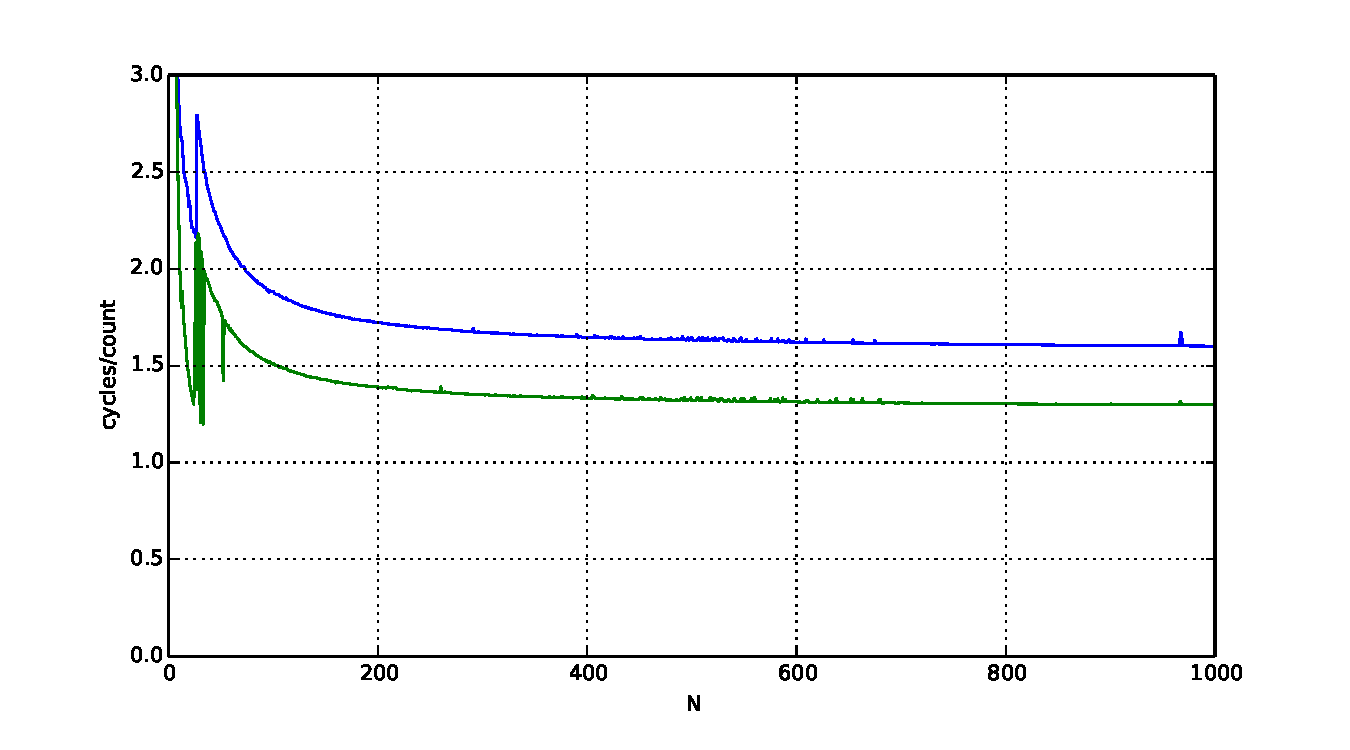
\includegraphics[height=0.8\textheight]{../optimization/sumrows-vary-novect}
\end{frame}

\begin{frame}{aliasing and performance (2) / GCC 5.4 -O3}
    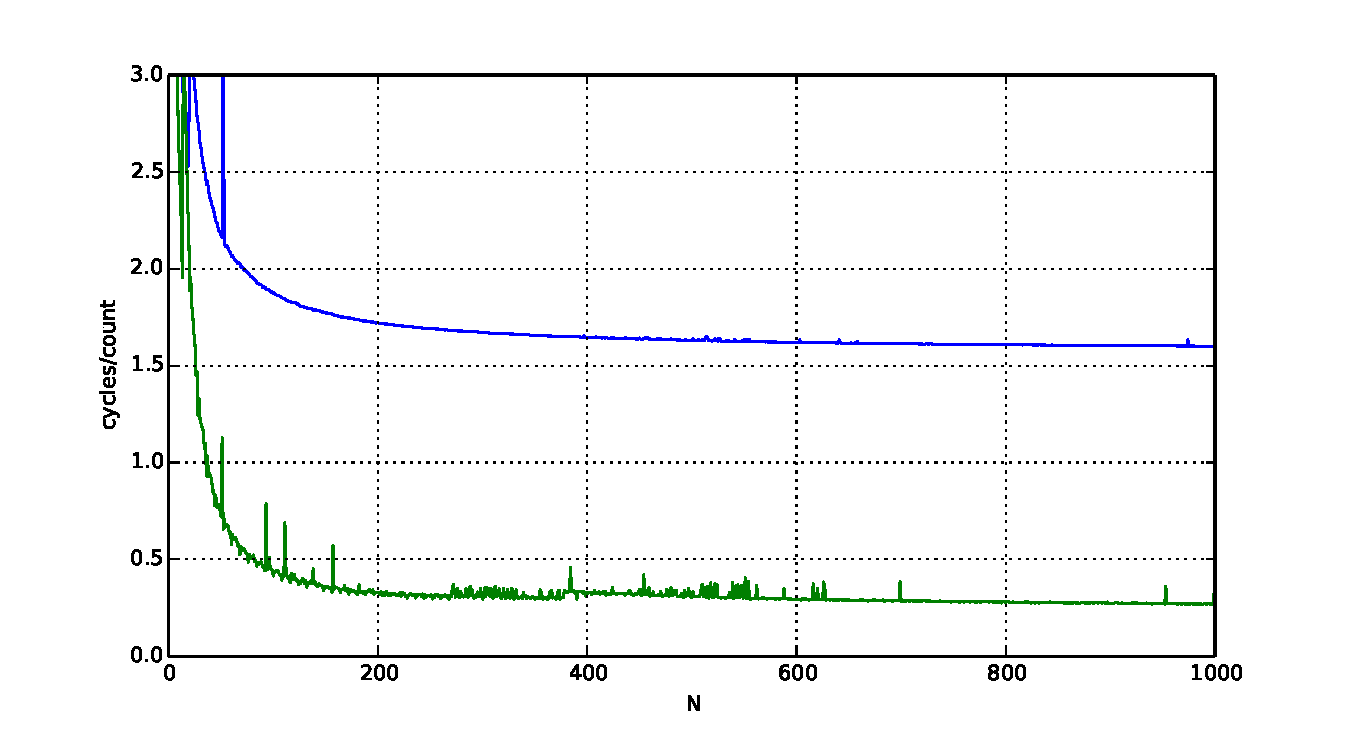
\includegraphics[height=0.8\textheight]{../optimization/sumrows-vary-vect}
\end{frame}


\subsection{avoiding aliasing}
\begin{frame}[fragile,label=registerReuseAuto2]{automatic register reuse}
\begin{itemize}
\item Compiler would need to generate overlap check:
\end{itemize}
\lstset{style=smaller,language=C}
\begin{lstlisting}
if (result > matrix + N * N || result < matrix) {
    for (int row = 0; row < N; ++row) {
        int sum = 0; /* kept in register */
        for (int col = 0; col < N; ++col)
            sum += matrix[row * N + col];
        result[row] = sum;
    }
} else {
    for (int row = 0; row < N; ++row) {
        result[row] = 0;
        for (int col = 0; col < N; ++col)
            result[row] += matrix[row * N + col];
        }
    }
}
\end{lstlisting}
\end{frame}

\subsection{`register blocking'}

\begin{frame}[fragile,label=blockingAliasing]{aliasing problems with cache blocking}
\lstset{
    style=small,
    language=C
}
\begin{lstlisting}
  for (int k = 0; k < N; k++) {
    for (int i = 0; i < N; i += 2) {
      for (int j = 0; j < N; j += 2) {
        C[(i+0)*N + j+0] += A[i*N+k] * B[k*N+j];
        C[(i+1)*N + j+0] += A[(i+1)*N+k] * B[k*N+j];
        C[(i+0)*N + j+1] += A[i*N+k] * B[k*N+j+1];
        C[(i+1)*N + j+1] += A[(i+1)*N+k] * B[k*N+j+1];
      }
    }
  }
\end{lstlisting}
\begin{itemize}
    \item can compiler keep \lstinline|A[i*N+k]| in a register?
\end{itemize}
\end{frame}



\begin{frame}[fragile,label=registerBlocking]{``register blocking''}
\lstset{
    style=small,
    language=C
}
\begin{lstlisting}
  for (int k = 0; k < N; ++k) {
    for (int i = 0; i < N; i += 2) {
      float Ai0k = A[(i+0)*N + k];
      float Ai1k = A[(i+1)*N + k];
      for (int j = 0; j < N; j += 2) {
        float Bkj0 = B[k*N + j+0];
        float Bkj1 = B[k*N + j+1];
        C[(i+0)*N + j+0] += Ai0k * Bkj0;
        C[(i+1)*N + j+0] += Ai1k * Bkj0;
        C[(i+0)*N + j+1] += Ai0k * Bkj1;
        C[(i+1)*N + j+1] += Ai1k * Bkj1;
      }
    }
  }
\end{lstlisting}
\end{frame}

 

\subsection{aliasing exercise}
\begin{frame}[fragile,label=aliasingEx]{aliasing exercise}
\begin{lstlisting}[language=C++,style=smaller]
void add(int *s1, int *s2, int *d) {
    for (int i = 0; i < 1000; ++i)
        d[i] = s1[i] + s2[i];
}
\end{lstlisting}
\hrule
The compiler \textbf{cannot} generate code equivalent to this:
\begin{lstlisting}[language=C++,style=smaller]
void add(int *s1, int *s2, int *d) {
    for (int i = 0; i < 1000; i += 2) {
        int temp1 = s1[i] + s2[i];
        int temp2 = s1[i+1] + s2[i+1];
        d[i] = temp1; d[i+1] = temp2;
    }
}
\end{lstlisting}
Which is an example of a call where the results could disagree:
{\small
\begin{tabular}{lll}
A. \texttt{add(\&A[0], \&A[1], \&B[0])} & B. \texttt{add(\&A[0], \&A[0], \&A[1])} \\
C. \texttt{add(\&B[0], \&A[10], \&A[0])} & D. \texttt{add(\&A[1000], \&A[1001], \&A[0])} \\
\end{tabular}
}
{\small (assume A, B are distinct, large arrays)}
\end{frame}

\begin{frame}<0>[fragile,label=aliasingExExplain]{aliasing exercise}
recall: s1=s2=A+0; d=A+1
\begin{lstlisting}[language=C++,style=smaller]
for (int i = 0; i < 1000; ++i)
    d[i] = s1[i] + s2[i];

/* i = 0: */ A[1] = A[0] + A[0];
/* i = 1: */ A[2] = A[1] + A[1];
\end{lstlisting}
\hrule
\begin{lstlisting}[language=C++,style=smaller]
for (int i = 0; i < 1000; i += 2) {
    temp1 = s1[i] + s2[i];
    temp2 = s1[i] + s2[i];
    d[i] = temp1;
    d[i+1] = temp2;

/* i = 0: */ temp1 = A[0] + A[0];
             temp2 = A[1] + A[1];
             A[1] = temp1;
             A[2] = temp2;
\end{lstlisting}
\end{frame}

\iftoggle{heldback}{}{\againframe<1>{aliasingExExplain}}


\subsection{aliasing as cache blocking problem}
\begin{frame}[fragile,label=loopOrder]{aliasing and cache optimizations}
    \lstset{language=C,style=small}
\begin{lstlisting}
for (int k = 0; k < N; ++k)
  for (int i = 0; i < N; ++i)
    for (int j = 0; j < N; ++j)
      C[i*N+j] += A[i * N + k] * B[k * N + j];
\end{lstlisting}
\hrulefill
\begin{lstlisting}
for (int i = 0; i < N; ++i)
  for (int j = 0; j < N; ++j)
    for (int k = 0; k < N; ++k)
      C[i*N+j] += A[i * N + k] * B[k * N + j];
\end{lstlisting}
    \begin{itemize}
        \item \lstinline|C = A|? \lstinline|C = &A[10]|?
        \item compiler can't generate same code for both
    \end{itemize}
\end{frame}



\subsection{compiler limits and loop optimizations} % FIXME: skip if not time:
\begin{frame}[fragile,label=loopUnrollDown]{loop unrolling downsides}
    \begin{itemize}
    \item bigger executables $\rightarrow$ instruction cache misses
    \item slower if small number of loop iterations
        \begin{itemize}
        \item extra code to handle leftovers, etc.
        \end{itemize}
    \vspace{.5cm}
    \item want to unroll loops that are run a lot and quick to execute
    \item problem: compiler probably can't tell if this meets those criteria
    \end{itemize}
\begin{lstlisting}[language=C,style=small]
  for (int i = 0; i < some_variable; ++i) {
    sum += some_function();
  }
\end{lstlisting}
\end{frame}

\begin{frame}[fragile,label=loopUnrollDiff]{figuring out how to unroll?}
exercise: why can the compiler probably not do this transformation?
\begin{lstlisting}[language=C,style=smaller]
void foo() { int sum = 0;
  for (int i = 0; i < some_global_variable; ++i) {
    sum += some_function();
  }
}
\end{lstlisting}
\hrule
\begin{lstlisting}[language=C,style=smaller]
void foo_transformed() { int sum = 0;
  int i = 0;
  if (some_global_variable % 2 == 1) {
    i += 1;
    sum += some_function();
  }
  for (; i < some_global_variable; i += 2) {
    sum += some_function();
    sum += some_function();
  }
}
\end{lstlisting}
\end{frame}

\begin{frame}[fragile,label=multAccDown]{multiple accumulators downsides}
    \begin{itemize}
    \item downsides of loop unrolling 
        \begin{itemize}
        \item bigger executables, slower if small number of iterations
        \end{itemize}
    \item + uses extra registers (can't use those regs for something else)
    \vspace{.5cm}
    \item want to use multiple accumulators if latency likely bottleneck
    \item problem: compiler probably can't tell if this meets those criteria
    \end{itemize}
\begin{lstlisting}[language=C,style=small]
  for (int i = 0; i < some_variable; ++i) {
    sum += some_function();
  }
\end{lstlisting}
\end{frame}


\section{inlining}
\begin{frame}[fragile,label=inliningMot]{loop with a function call}
\lstset{language=C,style=smaller,
    moredelim=**[is][\btHL<2>]{~2~}{~end~},
    }
\begin{lstlisting}
int addWithLimit(int x, int y) {
    int total = x + y;
    if (total > 10000)
        return 10000;
    else
        return total;
}
...
int sum(int *array, int n) {
    int sum = 0;
    for (int i = 0; i < n; i++)
        sum = ~2~addWithLimit~end~(sum, array[i]);
    return sum;
}
\end{lstlisting}
\end{frame}

\begin{frame}[fragile,label=inlining]{function call assembly}
\lstset{language=myasm,style=small,
    moredelim=**[is][\btHL<2>]{~2~}{~end~},
    }
\begin{lstlisting}
    ... loop stuff ...
    movl (%rbx), %esi // mov array[i]
    movl %eax, %edi   // mov sum
    call addWithLimit
    ... more loop stuff ...
    ...
addWithLimit:
    ... /* code here */
    ret
\end{lstlisting}
    \begin{itemize}
        \item extra instructions executed: two moves, a call, and a ret
        \item<2-> alternative: \textit{inline} the call
    \end{itemize}
\begin{visibleenv}<2->
\begin{lstlisting}
    ... loop stuff ...
    ... /* code here (+ small changes for arguments
                        being in different places) */
    ... more loop stuff ...
\end{lstlisting}
\end{visibleenv}
\end{frame}

\begin{frame}[fragile,label=manualInlining]{manual inlining}
\begin{lstlisting}
int sum(int *array, int n) {
    int sum = 0;
    for (int i = 0; i < n; i++) {
        sum = sum + array[i];
        if (sum > 10000)
            sum = 10000;
    }
    return sum;
}

\end{lstlisting}
\end{frame}

% FIXME: #define

\begin{frame}[fragile,label=inlineProCon]{inlining pro/con}
    \begin{itemize}
        \item avoids call, ret, extra move instructions
        \item allows compiler to \myemph{use more registers}
            \begin{itemize}
            \item no caller-saved register problems
            \end{itemize}
        \vspace{.5cm}
        \item but not always faster:
        \item worse for instruction cache
            \begin{itemize}
            \item (more copies of function body code)
            \end{itemize}
    \end{itemize}
\end{frame}

\begin{frame}{compiler inlining}
    \begin{itemize}
    \item compilers will inline, but\ldots
    \item will usually \myemph{avoid making code much bigger}
        \begin{itemize}
        \item heuristic: inline if function is small enough
        \item heuristic: inline if called exactly once
        \end{itemize}
    \item will usually \myemph{not inline across .o files}
    \vspace{.5cm}
    \item some compilers allow hints to say ``please inline/do not inline this function''
    \end{itemize}
\end{frame}



\againframe<3>{compileLimits}

\section{loop hoisting}
\begin{frame}[fragile,label=redundCalc1]{remove redundant operations (1)}
    \lstset{language=C,style=small}
\begin{lstlisting}
int number_of_As(const char *str) {
    int count = 0;
    for (int i = 0; i < strlen(str); ++i) {
        if (str[i] == 'a')
            count++;
    }
    return count;
}
\end{lstlisting}
\end{frame}

\begin{frame}[fragile,label=redundCalc1Fix]{remove redundant operations (1, fix)}
    \lstset{language=C,style=small,
    moredelim=**[is][\btHL<all:2>]{~2~}{~end~},
    }
\begin{lstlisting}
int number_of_As(const char *str) {
    int count = 0;
    int length = ~2~strlen(str)~end~;
    for (int i = 0; i < length; ++i) {
        if (str[i] == 'a')
            count++;
    }
    return count;
}
\end{lstlisting}
    \begin{itemize}
        \item call strlen once, not once per character!
        \item Big-Oh improvement!
    \end{itemize}
\end{frame}

\begin{frame}[fragile,label=removeRedundant2]{remove redundant operations (2)}
    \lstset{language=C,style=small,
    moredelim=**[is][\btHL<all:2>]{~2~}{~end~},
    }
\begin{lstlisting}
int shiftArray(int *source, int *dest, int N, int amount) {
    for (int i = 0; i < N; ++i) {
        if (i + amount < N)
            dest[i] = source[i + amount];
        else
            dest[i] = source[N - 1];
    }
}
\end{lstlisting}
    \begin{itemize}
    \item compare i + amount to N many times
    \end{itemize}
\end{frame}

\begin{frame}[fragile,label=removeRedundant2Fix]{remove redundant operations (2, fix)}
    \lstset{language=C,style=small,
    moredelim=**[is][\btHL<all:2>]{~2~}{~end~},
    }
\begin{lstlisting}
int shiftArray(int *source, int *dest, int N, int amount) {
    int i;
    for (i = 0; i + amount < N; ++i) {
        dest[i] = source[i + amount];
    }
    for (; i < N; ++i) {
        dest[i] = source[N - 1];
    }
}
\end{lstlisting}
    \begin{itemize}
    \item eliminate comparisons
    \end{itemize}
\end{frame}


\againframe<4>{compileLimits}

\section{exercise: which hurts\ldots}
\begin{frame}{exercise: when optimizations backfire\ldots}
Which of these optimizations are likely to \textbf{increase} 
machine code size? (\textbf{Select all that apply.})
\vspace{1cm}

Which of these optimizations are likely to \textbf{increase}
number of instructions executed? (\textbf{Select all that apply.})
\vspace{1cm}

\begin{tabular}{lll}
A. cache blocking & B. function inlining & C. loop unrolling \\
\multicolumn{3}{l}{D. moving a calculation outside a loop} \\
\multicolumn{3}{l}{E. multiple accumulators (after loop unrolling)} \\
\end{tabular}
\end{frame}


\section{vector instructions}
\begin{frame}{looplab speeds on my desktop}
    \begin{itemize}
    \item original assembly: 2.0 cycles/element
    \item unrolled x2: 1.0 cycles element
    \item unrolled x4: 1.0 cycles element
    \item unrolled x8: 1.0 cycles element
    \item unrolled x8, 4 accumulators: 0.5 cycles element
    \vspace{.5cm}
    \item<2-> Clang 6 optimized code: 0.13 cycles/element
    \item<2-> GCC optimized code: 0.14 cycles/element
    \vspace{.5cm}
    \item<3-> how? instructions that add \textit{16 pairs of shorts} at once!
        \begin{itemize}
            \item ``vector' or ``SIMD'' {\scriptsize(single instruction multiple data)} instruction
        \end{itemize}
    \end{itemize}
\end{frame}


\subsection{add example}
\begin{frame}[fragile,label=unvectAdd]{unvectorized add (original)}
\begin{lstlisting}[language=C++,style=small]
unsigned int A[512], B[512];
...
for (int i = 0; i < N; i += 1) {
    A[i] = A[i] + B[i];
}
\end{lstlisting}
\end{frame}

\begin{frame}[fragile,label=unvectAddUnrolled]{unvectorized add (unrolled)}
\begin{lstlisting}[language=C++,style=small]
unsigned int A[512], B[512];
...
for (int i = 0; i < 512; i += 8) {
    A[i+0] = A[i+0] + B[i+0];
    A[i+1] = A[i+1] + B[i+1];
    A[i+2] = A[i+2] + B[i+2];
    A[i+3] = A[i+3] + B[i+3];
    A[i+4] = A[i+4] + B[i+4];
    A[i+5] = A[i+5] + B[i+5];
    A[i+6] = A[i+6] + B[i+6];
    A[i+7] = A[i+7] + B[i+7];
}
\end{lstlisting}
\begin{itemize}
\item goal: use SIMD add instruction to do all 8 adds above
    \begin{itemize}
    \item SIMD = single instruction, multiple data
    \end{itemize}
\end{itemize}
\end{frame}



\subsection{assembly}

\begin{frame}[fragile,label=vecAddAsm]{desired assembly}
\begin{lstlisting}[language=myasm,style=small]
  xor %rax, %rax
the_loop:
  vmovdqu A(%rax), %ymm0      /* load 256 bits of A into ymm0 */
  vmovdqu B(%rax), %ymm1      /* load 256 bits of B into ymm1 */
  vpaddd %ymm1, %ymm0, %ymm0  /* ymm1 + ymm0 -> ymm0 */
  vmovdqu %ymm0, A(%rax)  /* store ymm0 into A */
  addq $32, %rax              /* increment index by 32 bytes */
  cmpq $2048, %rax            /* offset < 2048 (= 512 * 4) bytes */
  jne the_loop
\end{lstlisting}
\end{frame}


\subsection{vector instruction operation}
\usetikzlibrary{arrows.meta,calc}

\begin{frame}{vector add picture}
\begin{tikzpicture}
\tikzset{>=Latex}
\newcommand{\myfactor}{.73}
\draw[fill=blue!20,thick] (1, 0) rectangle (14, 1);
\draw[fill=green!20,thick] (1, 3) rectangle (14, 4);
\foreach \y in {3,4,5,6,7,...,16,17} {
    \pgfmathsetmacro\x{\y * \myfactor}
    \draw (\x, 0) -- (\x, 1);
    \node[font=\fontsize{8.5}{9.5}\selectfont] at ($(\x, 0.5) + (.4, 0)$) {A[\y]};
    \draw (\x, 3) -- (\x, 4);
    \node[font=\fontsize{8.5}{9.5}\selectfont] at ($(\x, 3.5) + (.4, 0)$) {B[\y]};
}
    \draw (18 * \myfactor,0) --++ (0, 1);
    \draw (18 * \myfactor,3) --++ (0, 1);
    \node[font=\small] at (19 *\myfactor, .5) {\ldots};
    \node[font=\small] at (19 *\myfactor, 3.5) {\ldots};
    \node[font=\small] at (1.5, .5) {\ldots};
    \node[font=\small] at (1.5, 3.5) {\ldots};

\draw[ultra thick] (8 * \myfactor, 0) rectangle (16 * \myfactor, 1);
\draw[ultra thick] (8 * \myfactor, 3) rectangle (16 * \myfactor, 4);
\draw[->,very thick] (7, 0) |- ++(2.5cm, -.5cm) node[left,fill=white] {vmovdqu}
                            -- ++(.5cm, 0cm) node[right] (xmm0) {\%ymm0};        

\draw[->,very thick] (7, 3) |- ++(2.5cm, -.5cm) node[left,fill=white] {vmovdqu}
                            -- ++(.5cm, 0cm) node[right] (xmm1) {\%ymm1};        

\draw[->,very thick] (xmm0.east) -- ++(2cm,0cm) node[right,fill=white] (paddd){vpaddd};
\draw[->,very thick] (xmm1.east) -| (paddd.north);

\draw[->,very thick] (paddd.south) |- ++(-2cm, -2cm) node[left] (ymm0Final) {\%ymm0};

\begin{scope}[shift={(ymm0Final.west)}]
\draw[fill=yellow!20,very thick] (0,-1) rectangle (-\myfactor * 8, 1.0);
\foreach \x/\y in {8,9,10,11,12,13,14,15} {
    \pgfmathsetmacro\x{-(15-\y+8-7)*\myfactor}
    \draw (\x, -1) -- (\x, 1);
    \node[font=\fontsize{9}{10}\selectfont,align=center] at ($(\x, 0) + (.4, 0)$) {A[\y]\\+\\B[\y]};
}
\end{scope}
\end{tikzpicture}
\end{frame}


\subsection{hardware for vector instructions}
\usetikzlibrary{chains,positioning,fit}
\begin{frame}{one view of vector functional units}
    \begin{tikzpicture}
\tikzset{
    every node/.style={font=\small},
    >=Latex,
    stage/.style={draw,rectangle,align=center,minimum height=1cm},
    stageSmall/.style={draw,rectangle,align=center,minimum height=.75cm},
    stageTall/.style={draw,rectangle,align=center,minimum height=2.2cm},
    iqueue/.style={fill=blue!30,align=center,draw,rectangle split,rectangle split horizontal,rectangle split parts=3,
        inner sep=.5mm,minimum height=4.0cm},
    buffer/.style={fill=blue!30,align=center,draw,rectangle split,rectangle split parts=5, inner sep=.5mm},
    hi/.style={red,ultra thick,draw},
    every label/.style={align=center,red!50!black},
}
\begin{scope}[start chain=going right,every join/.style={->,thick},node distance=5mm]
\node[stageSmall,on chain,anchor=north] (mult11) {ALU (lane 1) \\ (stage 1)};
\node[stageSmall,on chain,join] (mult12) {ALU (lane 1) \\ (stage 2)};
\node[stageSmall,on chain,join] (mult13) {ALU (lane1) \\ (stage 3)};
\end{scope}
\begin{scope}[start chain=going right,every join/.style={->,thick},node distance=5mm]
    \node[stageSmall,on chain,anchor=north] (mult21) at ([yshift=-.5cm]mult11.south) {ALU (lane 2) \\ (stage 1)};
\node[stageSmall,on chain,join] (mult22) {ALU (lane 2) \\ (stage 2)};
\node[stageSmall,on chain,join] (mult23) {ALU (lane 2) \\ (stage 3)};
\end{scope}
\begin{scope}[start chain=going right,every join/.style={->,thick},node distance=5mm]
    \node[stageSmall,on chain,anchor=north] (mult31) at ([yshift=-.5cm]mult21.south) {ALU (lane 3) \\ (stage 1)};
\node[stageSmall,on chain,join] (mult32) {ALU (lane 3) \\ (stage 2)};
\node[stageSmall,on chain,join] (mult33) {ALU (lane 3) \\ (stage 3)};
\end{scope}
\begin{scope}[start chain=going right,every join/.style={->,thick},node distance=5mm]
\node[stageSmall,on chain,anchor=north] (mult41) at ([yshift=-.5cm]mult31.south) {ALU (lane 4) \\ (stage 1)};
\node[stageSmall,on chain,join] (mult42) {ALU (lane 4) \\ (stage 2)};
\node[stageSmall,on chain,join] (mult43) {ALU (lane 4) \\ (stage 3)};
\end{scope}
        \node [left=1cm of mult11,align=right] (valueInput) {input values \\ (one/cycle)};
        \node [right=1cm of mult13,align=left] (valueOutput) {output values \\ (one/cycle)};
        \draw[->,thick] (valueInput) -- (mult11);
        \draw[->,thick] (mult13) -- (valueOutput);
        \draw[->,thick] (valueInput.east |- mult21.east) -- (mult21);
        \draw[->,thick] (mult23) -- (valueOutput.west |- mult23.east);
        \draw[->,thick] (valueInput.east |- mult31.east) -- (mult31);
        \draw[->,thick] (mult33) -- (valueOutput.west |- mult33.east);
        \draw[->,thick] (valueInput.east |- mult41.east) -- (mult41);
        \draw[->,thick] (mult43) -- (valueOutput.west |- mult41.east);
        \node[draw,dashed,fit=(mult11) (mult43),label={south:vector ALU}] {};
    \end{tikzpicture}
\end{frame}

\begin{frame}{why vector instructions?}
    \begin{itemize}
        \item lots of logic not dedicated to computation
            \begin{itemize}
            \item instruction queue
            \item reorder buffer
            \item instruction fetch
            \item branch prediction
            \item \ldots
            \end{itemize}
        \item adding vector instructions --- \myemph{little extra control logic}
        \item \ldots but \myemph{a lot more computational capacity}
    \end{itemize}
\end{frame}



\subsection{autovectorization?}


\begin{frame}[fragile,label=explicitVec]{vector instructions and compilers}
\begin{itemize}
    \item compilers can sometimes figure out how to use vector instructions
        \begin{itemize}
        \item (and have gotten much, much better at it over the past decade)
        \end{itemize}
    \item but easily messsed up:
    \begin{itemize}
        \item by aliasing
        \item by conditionals
        \item by some operation with no vector instruction
        \item \ldots
    \end{itemize}
\end{itemize}
\end{frame}



\subsection{vector instructions are fickle}
\begin{frame}[fragile,label=vectFickle1]{fickle compiler vectorization (1)}
    \lstset{language=C,style=smaller}
    \begin{itemize}
    \item GCC 8.2 and Clang 7.0 generate vector instructions for this:
\begin{lstlisting}
#define N 1024
void foo(unsigned int *A, unsigned int *B) {
    for (int k = 0; k < N; ++k)
        for (int i = 0; i < N; ++i)
            for (int j = 0; j < N; ++j)
                B[i * N + j] += A[i * N + k] * A[k * N + j];
}
\end{lstlisting}
\item but not:
\begin{lstlisting}
#define N 1024
void foo(unsigned int *A, unsigned int *B) {
    for (int i = 0; i < N; ++i)
        for (int j = 0; j < N; ++j)
            for (int k = 0; k < N; ++k)
                B[i * N + j] += A[i * N + k] * A[j * N + k];
}
\end{lstlisting}
    \end{itemize}
\end{frame}

\begin{frame}[fragile,label=vectFickle2]{fickle compiler vectorization (2)}
    \lstset{language=C,style=smaller}
    \begin{itemize}
    \item Clang 5.0.0 generates vector instructions for this:
\begin{lstlisting}
void foo(int N, unsigned int *A, unsigned int *B) {
    for (int k = 0; k < N; ++k)
        for (int i = 0; i < N; ++i)
            for (int j = 0; j < N; ++j)
                B[i * N + j] += A[i * N + k] * A[k * N + j];
}
\end{lstlisting}
\item but not: (fixed in later versions)
\begin{lstlisting}
void foo(long N, unsigned int *A, unsigned int *B) {
    for (long k = 0; k < N; ++k)
        for (long i = 0; i < N; ++i)
            for (long j = 0; j < N; ++j)
                B[i * N + j] += A[i * N + k] * A[k * N + j];
}
\end{lstlisting}
    \end{itemize}
\end{frame}
% https://godbolt.org/g/q5qGrM


\subsection{vector instrinsics: why}
\begin{frame}[fragile,label=vecIntr]{vector intrinsics}
\begin{itemize}
    \item if compiler doesn't work\ldots
    \item could write vector instruction assembly by hand
    \vspace{.5cm}
    \item second option: ``intrinsic functions''
    \item C functions that compile to particular instructions
\end{itemize}
\end{frame}


\subsection{add example}
\begin{frame}[fragile,label=intrSum]{vector intrinsics: add example}
\lstset{
    language=C,
    style=small,
    moredelim=**[is][\btHL<all:2>]{~2~}{~end~},
    moredelim=**[is][\btHL<all:3>]{~3~}{~end~},
    moredelim=**[is][\btHL<all:4>]{~4~}{~end~},
    morekeywords={\_\_m256i},
}
\begin{lstlisting}
int A[512], B[512];

for (int i = 0; i < 512; i += 8) {
  // "si256" --> 256 bit integer
  // a_values = {A[i], A[i+1], ..., A[i+7]} (8 x 32 bits)
  ~2~__m256i~end~ a_values = ~3~_mm256_loadu_si256~end~((~2~__m256i~end~*) &A[i]);
  // b_values = {B[i], B[i+1] ..., A[i+7]} (8 x 32 bits)
  ~2~__m256i~end~ b_values = ~3~_mm256_loadu_si256~end~((~2~__m256i~end~*) &B[i]);
 
  // add eight 32-bit integers
  // sums = {A[i] + B[i], A[i+1] + B[i+1], ...., A[i+7] + B[i+7]}
  ~2~__m256i~end~ sums = ~4~_mm256_add_epi32~end~(a_values, b_values);
 
  // {A[i], A[i+1], A[i+2], A[i+3], ..., A[i+7]} = sums
  ~3~_mm256_storeu_si256~end~((~2~__m256i~end~*) &A[i], sums);
}
\end{lstlisting}
\begin{tikzpicture}[overlay,remember picture]
\coordinate (infoBox) at ([yshift=-1cm]current page.north);
\begin{visibleenv}<all:2>
    \node[draw=red,ultra thick,anchor=north,fill=white,align=left] at (infoBox) {
        special type {\tt \_\_m256i} --- ``256 bits of integers'' \\
        other types: {\tt \_\_m256} (floats), {\tt \_\_m128d} (doubles)
    };
\end{visibleenv}

\begin{visibleenv}<all:3>
    \node[draw=red,ultra thick,anchor=north,align=left,fill=white] at (infoBox) {
        functions to store/load \\
        {\tt si256} means ``256-bit integer value'' \\
        {\tt u} for ``unaligned'' (otherwise, pointer address must be multiple of 32) 
    };
\end{visibleenv}

\begin{visibleenv}<4>
    \node[draw=red,ultra thick,anchor=north,align=left,fill=white] at ([yshift=-2cm]infoBox) {
        function to add \\
        {\tt epi32} means ``8 32-bit integers''
    };
\end{visibleenv}
\end{tikzpicture}
\end{frame}

\begin{frame}[fragile,label=intrSizes]{vector intrinsics: different size}
\lstset{
    language=C,
    style=small,
    moredelim=**[is][\btHL<all:2>]{~2~}{~end~},
    moredelim=**[is][\btHL<all:3>]{~3~}{~end~},
    moredelim=**[is][\btHL<all:4>]{~4~}{~end~},
    morekeywords={\_\_m128i},
}
\begin{lstlisting}
~2~long~end~ A[512], B[512]; /* instead of int */
...
for (int i = 0; i < 512; i += ~2~4~end~) {
  // a_values = {A[i], A[i+1], A[i+2], A[i+3]} (4 x 64 bits)
   __m256i a_values = _mm256_loadu_si256((__m256i*) &A[i]);
  // b_values = {B[i], B[i+1], B[i+2], B[i+3]} (4 x 64 bits)
   __m256i b_values = _mm256_loadu_si256((__m256i*) &B[i]);
   // add four 64-bit integers: vpaddq %ymm0, %ymm1
   // sums = {A[i] + B[i], A[i+1] + B[i+1], ...}
   __m256i sums = _mm256_add_~2~epi64~end~(a_values, b_values);
   // {A[i], A[i+1], A[i+2], A[i+3]} = sums
   _mm256_storeu_si256((__m256i*) &A[i], sums);
}
\end{lstlisting}
\end{frame}

\usetikzlibrary{arrows.meta,calc}

\begin{frame}{vector add picture (intrinsics)}
\begin{tikzpicture}
\tikzset{
    >=Latex,
    code label/.style={font=\small,align=center},
    element label/.style={font=\fontsize{7.5}{8.5}\selectfont},
}
\newcommand{\myfactor}{.7}
\draw[fill=blue!20,thick] (2, 0) rectangle (13.5, 1);
\draw[fill=green!20,thick] (2, 3) rectangle (13.5, 4);
\foreach \y in {4,5,6,7,...,16,17} {
    \pgfmathsetmacro\x{\y * \myfactor}
    \draw (\x, 0) -- (\x, 1);
    \node[element label] at ($(\x, 0.5) + (.4, 0)$) {A[\y]};
    \draw (\x, 3) -- (\x, 4);
    \node[element label] at ($(\x, 3.5) + (.4, 0)$) {B[\y]};
}
    \draw (18 * \myfactor,0) --++ (0, 1);
    \draw (18 * \myfactor,3) --++ (0, 1);
    \node[font=\small] at (18.5 *\myfactor, .5) {\ldots};
    \node[font=\small] at (18.5 *\myfactor, 3.5) {\ldots};
    \node[font=\small] at (2.5, .5) {\ldots};
    \node[font=\small] at (2.5, 3.5) {\ldots};

\draw[ultra thick] (8 * \myfactor, 0) rectangle (16 * \myfactor, 1);
\draw[ultra thick] (8 * \myfactor, 3) rectangle (16 * \myfactor, 4);
\draw[->,very thick] (7, 0) |- ++(2.5cm, -.9cm) node[left,fill=white,code label] {\_mm256\_loadu\_si256 \\ (asm: vmovdqu)}
                            -- ++(.5cm, 0cm) node[right,code label] (xmm0) {a\_values \\ (\%ymm0?)};        

\draw[->,very thick] (7, 3) |- ++(2.5cm, -.9cm) node[left,fill=white,code label] {\_mm256\_loadu\_si256 \\(asm: vmovdqu)}
                            -- ++(.5cm, 0cm) node[right,code label] (xmm1) {b\_values \\ (\%ymm1?)};        

\draw[->,very thick] (xmm0.east) -- ++(1cm,0cm) node[right,fill=white, code label] (paddd){\_mm256\_add\_epi32\\(asm: vpaddd)};
\draw[->,very thick] (xmm1.east) -| (paddd.north);

\draw[->,very thick] (paddd.south) |- ++(-2cm, -2cm) node[left,code label] (ymm0Final) {sum \\ (asm: \%ymm0?)};

\begin{scope}[shift={(ymm0Final.west)}]
\draw[fill=yellow!20,very thick] (0,-1) rectangle (-\myfactor * 8, 1.0);
\foreach \x/\y in {8,9,10,11,12,13,14,15} {
    \pgfmathsetmacro\x{-(15-\y+8-7)*\myfactor}
    \draw (\x, -1) -- (\x, 1);
    \node[element label,align=center] (final\y) at ($(\x, 0) + (.4, 0)$) {A[\y]\\+\\B[\y]};
}
\end{scope}
\begin{visibleenv}<2>
\draw[dotted,very thick,->] ([xshift=-1mm]final8.west) -- ++(-2cm,0cm) 
    |- (6, -0.3)  node[xshift=1.5cm,pos=0.25,code label,fill=white] {\_mm256\_storeu\_si256 \\ vmovups} -- (6, 0);
\end{visibleenv}
\end{tikzpicture}
\end{frame}


\subsection{exercise}
\begin{frame}[fragile,label=vectExercise]{exercise}
\begin{lstlisting}[language=C++,style=smaller]
long foo[8] = {1,1,2,2,3,3,4,4};
long bar[8] = {2,2,2,3,3,3,4,4};
__mm256i foo0_as_vector = _mm256_loadu_si256((__m256i*)&foo[0])
__mm256i foo4_as_vector = _mm256_loadu_si256((__m256i*)&foo[4])
__mm256i bar0_as_vector = _mm256_loadu_si256((__m256i*)&bar[0])

__mm256i result = _mm256_add_epi64(foo0_as_vector, foo4_as_vector);
result = _mm256_mullo_epi64(result, bar0_as_vector);
_mm256_storeu_si256((__mm256i*) &bar[4], result);
\end{lstlisting}
Final value of bar array?
\small\tt
\begin{tabular}{ll}
A. \{2,2,2,3,12,12,24,24\} & B. \{2,2,2,3,15,15,28,28\} \\
C. \{2,2,2,3,10,10,20,20\} & D. \{12,12,24,24,3,3,4,4\} \\
E. \{14,14,26,27,3,3,4,4\} & F. \{14,14,26,27,12,12,24,24\} \\
G. something else \\
\end{tabular}
\end{frame}


\subsection{note on 128-bit version}
\begin{frame}[fragile,label=vect128]{128-bit version, too}
\begin{itemize}
\item history: 256-bit vectors added in extension called AVX (c. 2011)
\item before: 128-bit vectors added in extension called SSE (c. 1999)
\vspace{.5cm}
\item 128-bit intrinsics exist, too:
    \begin{itemize}
    \item \texttt{\_\_m256i} becomes \texttt{\_\_m128i}
    \item \texttt{\_mm256\_add\_epi32} becomes \texttt{\_mm\_add\_epi32}
    \item \texttt{\_mm256\_loadu\_si256} becomes \texttt{\_mm\_loadu\_si128}
    \end{itemize}
\end{itemize}
\end{frame}


\subsection{vectorizing matmul}
% vectorizing matmul

\begin{frame}[fragile,label=mmSerial]{matrix multiply}
\lstset{language=C,style=small}
\begin{lstlisting}
void matmul(unsigned int *A, unsigned int *B, unsigned int *C) {
    for (int k = 0; k < N; ++k)
        for (int i = 0; i < N; ++i)
            for (int j = 0; j < N; ++j)
                C[i * N + j] += A[i * N + k] * B[k * N + j];
}
\end{lstlisting}
(simple version, no cache blocking, no avoiding aliasing beteeen C, B, A,\ldots)
\end{frame}

\begin{frame}[fragile,label=sqSerialUnrolled]{matmul unrolled}
\lstset{language=C,style=smaller}
\begin{lstlisting}
void matmul(unsigned int *A, unsigned int *B, unsigned int *C) {
  for (int k = 0; k < N; ++k) {
    for (int i = 0; i < N; ++i)
      for (int j = 0; j < N; j += 8) {
        /* goal: vectorize this */
        C[i * N + j + 0] += A[i * N + k] * B[k * N + j + 0];
        C[i * N + j + 1] += A[i * N + k] * B[k * N + j + 1];
        C[i * N + j + 2] += A[i * N + k] * B[k * N + j + 2];
        C[i * N + j + 3] += A[i * N + k] * B[k * N + j + 3];
        C[i * N + j + 4] += A[i * N + k] * B[k * N + j + 4];
        C[i * N + j + 5] += A[i * N + k] * B[k * N + j + 5];
        C[i * N + j + 6] += A[i * N + k] * B[k * N + j + 6];
        C[i * N + j + 7] += A[i * N + k] * B[k * N + j + 7];
      }
}
\end{lstlisting}
(NB: would probably also want to do cache blocking\ldots)
\end{frame}

\begin{frame}[fragile,label=sqVectInstr]{handy intrinsic functions for matmul}
    \begin{itemize}
        \item {\tt \_mm256\_set1\_epi32} --- load eight copies of a 32-bit value into a 256-bit value
            \begin{itemize}
            \item instructions generated vary; one example: {\tt vmovd} + {\tt vpbroadcastd}
            \end{itemize}
        \item {\tt \_mm256\_mullo\_epi32} --- multiply eight pairs of 32-bit values, give lowest 32-bits of results
            \begin{itemize}
            \item generates {\tt vpmulld}
            \end{itemize}
    \end{itemize}
\end{frame}

\begin{frame}[fragile,label=sqSerialUnrolledExpand]{vectorizing matmul}
\lstset{language=C,style=smaller,
    moredelim=**[is][\btHL<all:2>]{~2~}{~end~},
    moredelim=**[is][\btHL<all:3>]{~3~}{~end~},
    moredelim=**[is][\btHL<all:4>]{~4~}{~end~},
    moredelim=**[is][\btHL<all:5>]{~5~}{~end~},
}
\begin{lstlisting}
/* goal: vectorize this */
~2~C[i * N + j + 0]~end~ ~5~+=~end~ ~4~A[i * N + k] *~end~ ~3~B[k * N + j + 0]~end~;
~2~C[i * N + j + 1]~end~ ~5~+=~end~ ~4~A[i * N + k] *~end~ ~3~B[k * N + j + 1]~end~;
...
~2~C[i * N + j + 6]~end~ ~5~+=~end~ ~4~A[i * N + k] *~end~ ~3~B[k * N + j + 6]~end~;
~2~C[i * N + j + 7]~end~ ~5~+=~end~ ~4~A[i * N + k] *~end~ ~3~B[k * N + j + 7]~end~;
\end{lstlisting}
\hrulefill
\begin{onlyenv}<all:2>
\begin{lstlisting}
// load eight elements from C
Cij = _mm256_loadu_si256((__m256i*) &C[i * N + j + 0]);
... // manipulate vector here
// store eight elements into C
_mm_storeu_si256((__m256i*) &C[i * N + j + 0], Cij);
\end{lstlisting}
\end{onlyenv}
\begin{onlyenv}<all:3>
\begin{lstlisting}
// load eight elements from B
Bkj = _mm256_loadu_si256((__m256i*) &B[k * N + j + 0]);
... // multiply each by B[i * N + k] here
\end{lstlisting}
\end{onlyenv}
\begin{onlyenv}<all:4>
\begin{lstlisting}
// load eight elements starting with B[k * n + j]
Bkj = _mm256_loadu_si256((__m256i*) &B[k * N + j + 0]);
// load eight copies of A[i * N + k]
Aik = _mm256_set1_epi32(A[i * N + k]);
// multiply each pair
multiply_results = _mm256_mullo_epi32(Aik, Bkj);
\end{lstlisting}
\end{onlyenv}
\begin{onlyenv}<all:5>
\begin{lstlisting}
Cij = _mm256_add_epi32(Cij, multiply_results);
// store back results
_mm256_storeu_si256(..., Cij);
\end{lstlisting}
\end{onlyenv}
\end{frame}



\begin{frame}[fragile,label=sqVectCode]{matmul vectorized}
\lstset{language=C,style=smaller,morekeywords={\_\_m256i},mathescape=true}
\begin{lstlisting}
__m256i Cij, Bkj, Aik, multiply_results;

// Cij = {$C_{i,j}$, $C_{i,j+1}$, $C_{i,j+2}$, ..., $C_{i,j+7}$}
Cij = _mm256_loadu_si256((__m256i*) &C[i * N + j]);
// Bkj = {$B_{k,j}$, $B_{k,j+1}$, $B_{k,j+2}$, ..., $B_{k,j+7}$}
Bkj = _mm256_loadu_si256((__m256i*) &B[k * N + j]);

// Aik = {$A_{i,k}$, $A_{i,k}$, ..., $A_{i,k}$}
Aik = _mm256_set1_epi32(A[i * N + k]);

// Aik_times_Bkj = {$A_{i,k}\times B_{k,j}$, $A_{i,k}\times B_{k,j+1}$, $A_{i,k}\times B_{k,j+2}$, ..., $A_{i,k}\times B_{k,j+7}$}
multiply_results = _mm256_mullo_epi32(Aij, Bkj);

// Cij= {$C_{i,j} + A_{i,k}\times B_{k,j}$, $C_{i,j+1} + A_{i,k}\times B_{k,j+1}$, ...}
Cij = _mm256_add_epi32(Cij, multiply_results);

// store Cij into C
_mm256_storeu_si256((__m256i*) &C[i * N + j], Cij);
\end{lstlisting}
\end{frame}



\subsection{exercise}
\begin{frame}[fragile,label=vectorExercise2A]{vector exercise (2a)}
\begin{lstlisting}[language=C++,style=smaller]
long A[1024], B[1024];
...
for (int i = 0; i < 1024; i += 1)
    for (int j = 0; j < 1024; j += 1)
        A[i] += B[i] * B[j];
\end{lstlisting}
\hrule
{\fontsize{9}{10}\selectfont (casts omitted below to reduce clutter:)}
\begin{lstlisting}[language=C++,style=smaller]
for (int i = 0; i < 1024; i += 4) {
    A_part = _mm256_loadu_si256(&A[i]);
    Bi_part = _mm256_loadu_si256(&B[i]);
    for (int j = 0; j < 1024; /* BLANK 1 */) {
        Bj_part = _mm256_/* BLANK 2 */;
        A_part = _mm256_add_epi64(A_part,
            _mm256_mullo_epi64(Bi_part, Bj_part));
    }
    _mm256_storeu_si256(&A[i], A_part);
}
\end{lstlisting}
\small
What goes in BLANK 1 and BLANK 2? \\
\begin{tabular}{ll}
A. j += 1, {\small\tt loadu\_si256(\&B[j])} & B. j += 4, {\small\tt loadu\_si256(\&B[j])} \\
C. j += 1, {\small \tt set1\_epi64(B[j])} & D. j += 4, {\small\tt set1\_epi64(B[j])} \\
\end{tabular}
\end{frame}

\begin{frame}<0>[fragile,label=vectEx2Soln]{vector exercise 2 explanation}
\begin{lstlisting}[
        language=C++,style=smaller,
        moredelim={**[is][\btHL<all:1>]{~1~}{~end~}},
]
for (int i = 0; i < 1024; i += 1)
    for (int j = 0; j < 1024; j += 1)
        A[i] += B[i] * B[j];
/* -- transformed into -- */
for (int i = 0; i < 1024; i += 4)
    for (int j = 0; j < 1024; j += 1) {
        A[i+0] += B[i+0] * ~1~B[j]~end~;
        A[i+1] += B[i+1] * ~1~B[j]~end~;
        A[i+2] += B[i+2] * ~1~B[j]~end~;
        A[i+3] += B[i+3] * ~1~B[j]~end~;
    }

/* not the much harder to vectorize: */
for (int i = 0; i < 1024; i += 1)
    for (int j = 0; j < 1024; j += 4) {
        A[i] += B[i] * B[j+0];
        A[i] += B[i] * B[j+1];
        A[i] += B[i] * B[j+2];
        A[i] += B[i] * B[j+3];
    }
\end{lstlisting}
\end{frame}

\iftoggle{heldback}{}{\againframe<1>{vectEx2Soln}}

\begin{frame}<0>[fragile,label=vectEx2SolnAlt]{vector exercise 2 explanation}
\begin{lstlisting}[
        language=C++,style=smaller,
        moredelim={**[is][\btHL<all:1>]{~1~}{~end~}},
]
/* and not the more expanded: */;
for (int i = 0; i < 1024; i += 4)
    for (int j = 0; j < 1024; j += 4) {
        A[i+0] += B[i+0] * ~1~B[j]~end~;
        A[i+1] += B[i+1] * ~1~B[j]~end~;
        A[i+2] += B[i+2] * ~1~B[j]~end~;
        A[i+3] += B[i+3] * ~1~B[j]~end~;
        A[i+0] += B[i+0] * ~1~B[j+1]~end~;
        A[i+1] += B[i+1] * ~1~B[j+1]~end~;
        A[i+2] += B[i+2] * ~1~B[j+1]~end~;
        A[i+3] += B[i+3] * ~1~B[j+1]~end~;
        ...
    }
\end{lstlisting}
\end{frame}


\subsection{moving values in vector}
\begin{frame}{moving values in vectors?}
\begin{itemize}
\item sometimes values aren't in the right place in vector
\item example:
\item have: [1, 2, 3, 4]
\item want: [3, 4, 1, 2]
\vspace{.5cm}
\item there are instructions/intrinsics for doing this
    \begin{itemize}
    \item called shuffling/swizzling/permute/\ldots
    \end{itemize}
\item sometimes might need combination of them
\item worst-case: could rearrange on stack\ldots, I guess
\end{itemize}
\end{frame}

\begin{frame}[fragile,label=exampleShuffle]{example shuffling operation (1)}
goal: [1, 2, 3, 4] to [3, 4, 1, 2] (64-bit values)
\begin{lstlisting}[language=C++,style=smaller]
/* x = {1, 2, 3, 4} */
__m256i x = _mm256_setr_epi64x(1, 2, 3, 4);
__m256i result = _mm256_permute4x64_epi64(
        x,
        /* index 2, then 3, then 0, then 1 */
        2 | (3 << 2) | (0 << 4) | (1 << 6)
        /* could also write _MM_SHUFFLE(1, 0, 3, 2) */
    );
/* result = {3, 4, 1, 2} */
\end{lstlisting}
\end{frame}


\subsection{other vector ISAs}
\begin{frame}{other vector instructions}
    \begin{itemize}
    \item multiple extensions to the X86 instruction set for vector instructions
    \item early versions (128-bit vectors): SSE, SSE2, SSE3, SSSE3, SSE4.1, SSE4.2
        \begin{itemize}
        \item 128-bit vectors
        \end{itemize}
    \item this class (256-bit): AVX, AVX2
    \item not this class (512+-bit): AVX-512
        \begin{itemize}
        \item 512-bit vectors
        \end{itemize}
    \item also other ISAs have these: e.g. NEON on ARM, MSA on MIPS, AltiVec/VMX on POWER, \ldots
    \item GPUs are essentially vector-instruction-specialized CPUs
    \end{itemize}
\end{frame}

\begin{frame}{other vector interfaces}
    \begin{itemize}
    \item intrinsics (our assignments) one way
    \item some alternate programming interfaces
        \begin{itemize}
        \item have compiler do more work than intrinsics
        \end{itemize}
    \item e.g. CUDA, OpenCL, GCC's vector instructions
    \end{itemize}
\end{frame}


\subsection{other vector instr. features}


\begin{frame}{other vector instructions features}
    \begin{itemize}
    \item more flexible vector instruction features:
        \begin{itemize}
        \item invented in the 1990s
        \item often present in GPUs and being rediscovered by modern ISAs
        \end{itemize}
    \item reasonable conditional handling
    \item better variable-length vectors
    \item ability to load/store non-contiguous values
    \vspace{.5cm}
    \item some of these features in AVX2/AVX512
    \end{itemize}
\end{frame}


\subsection{interfaces other than intrinisics}
\begin{frame}{alternate vector interfaces}
    \begin{itemize}
    \item intrinsics functions/assembly aren't the only way to write vector code
    \item e.g. GCC vector extensions: more like normal C code 
        \begin{itemize}
        \item types for each kind of vector
        \item write {\tt +} instead of {\tt \_mm\_add\_epi32}
        \end{itemize}
    \item e.g. CUDA (GPUs): looks like writing multithreaded code, \\ but each thread is vector ``lane''
    \end{itemize}
\end{frame}



\section{profilers}
\begin{frame}{optimizing real programs}
    \begin{itemize}
    \item ask your compiler to try first
    \vspace{.5cm}
    \item spend effort where \myemph{it matters}
    \item e.g. 90\% of program time spent reading files, but optimize computation?
    \item e.g. 90\% of program time spent in routine A, but optimize B?
    \end{itemize}
\end{frame}

\begin{frame}{profilers}
    \begin{itemize}
    \item first step --- tool to determine where you spend time
    \item tools exist to do this for programs
    \item example on Linux: \texttt{perf}
    \end{itemize}
\end{frame}

\begin{frame}{example}
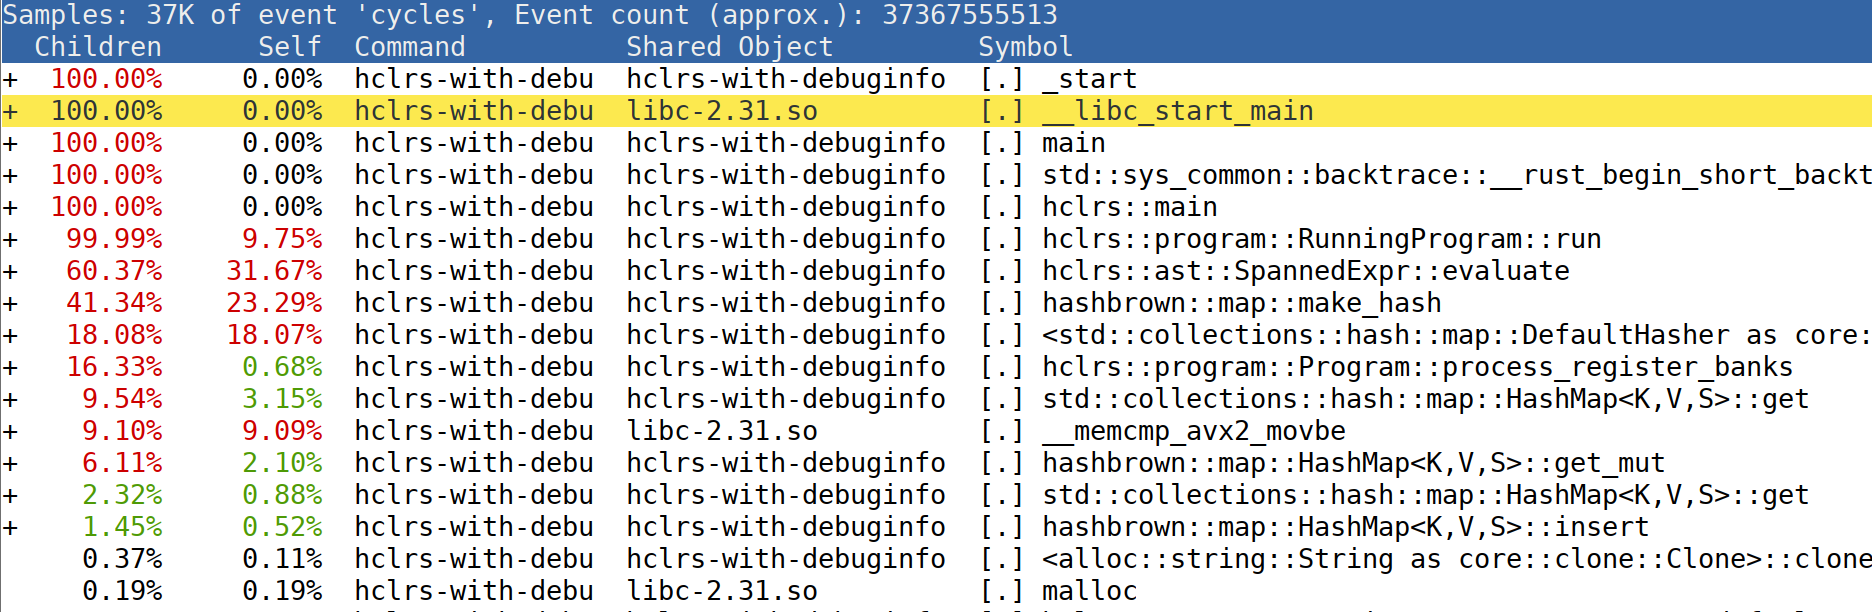
\includegraphics[width=\textwidth]{../optimization/perf-screenshot}
\end{frame}



\section{backup slides}
\begin{frame}{backup slides}
\end{frame}

\subsection{OOO: handling branch misprediction}
\againframe<15>{oooPipe}
\usetikzlibrary{arrows.meta,chains,fit,matrix,shapes.multipart}

\begin{frame}{reorder buffer: on rename}
\begin{tikzpicture}
\tikzset{
    every node/.style={font=\small},
    >=Latex,
    stage/.style={draw,rectangle,align=center,minimum height=1cm},
    stageSmall/.style={draw,rectangle,align=center,minimum height=.5cm,inner sep=0.5mm},
    stageTall/.style={draw,rectangle,align=center,minimum height=2.2cm,font=\fontsize{9.5}{10.5}\selectfont},
    iqueue/.style={fill=blue!30,align=center,draw,rectangle split,rectangle split horizontal,rectangle split parts=3,
        inner sep=.5mm,minimum height=4.0cm},
    buffer/.style={fill=blue!30,align=center,draw,rectangle split,rectangle split parts=5, inner sep=.5mm},
    hi/.style={red,ultra thick,draw},
    register map/.style={
        tight matrix,
        nodes={font=\fontsize{9}{10}\tt\selectfont},
        row 1/.style={nodes={font=\bfseries\small}},
        column 2/.append style={nodes={text width=1.7cm}}
    },
}
\matrix[
    anchor=north,
    register map,
    label={[alias=rename map label,align=center]north:phys $\rightarrow$ arch. reg \\ for new instrs},
] (rename map) {
    arch. reg \& phys. reg \\
    \%rax       \& \%x12 \\
    \%rcx       \& \%x17 \\
    \%rbx       \& \%x13 \\
    \%rdx       \& \sout<4->{\%x07}\only<4->{~\myemph<4>{\%x19}} \\
    \ldots    \& \ldots \\
};
\matrix[tight matrix,anchor=north west,
    label={[alias=free label]north:free list},
    nodes={font=\fontsize{9}{10}\tt\selectfont},
] (free list) at ([yshift=-1cm]rename map.south west)
{
    \sout<4->{\%x19} \\
    \%x23 \\
    \ldots \\
    \ldots \\
};
\begin{visibleenv}<2->
\matrix[
    anchor=north west,
    tight matrix,
    label={north:reorder buffer (ROB)},
    nodes={font=\fontsize{9}{10}\selectfont},
    row 1/.style={nodes={font=\bfseries\fontsize{8}{9}\selectfont,minimum height=.65cm}},
    row 12/.append style={nodes={alt=<4>{text=red}}},
    column 1/.append style={nodes={text width=.75cm}},
    column 2/.append style={nodes={text width=1cm,font=\fontsize{8}{9}\tt\selectfont}},
    column 3/.append style={nodes={text width=2cm,font=\fontsize{8}{9}\tt\selectfont}},
    column 4/.append style={nodes={text width=.75cm}},
    column 5/.append style={nodes={text width=1.5cm}}
] (rob) at ([xshift=6cm]rename map.north east) {
    instr num. \& PC \& dest. reg \& done? \& mispred? / except? \\
    |[alias=last instr loc]| 14 \& 0x1233 \& \%rbx / \%x23 \& ~ \& ~ \\ 
    15 \& 0x1239 \& \%rax / \%x30 \& ~ \& ~ \\ 
    16 \& 0x1242 \& \%rcx / \%x31 \& ~ \& ~ \\ 
    17 \& 0x1244 \& \%rcx / \%x32 \& ~ \& ~ \\ 
    18 \& 0x1248 \& \%rdx / \%x34 \& ~ \& ~ \\
    19 \& 0x1249 \& \%rax / \%x38 \& ~ \& ~ \\
    20 \& 0x1254 \& PC \&  ~ \& ~ \\
    21 \& 0x1260 \& \%rcx / \%x17 \& ~ \& ~ \\
    \ldots \& \ldots \& \ldots \& \ldots \& \ldots \\
    31 \& 0x129f \& \%rax / \%x12 \& ~ \& ~ \\
    |[alias=new instr loc]| \alt<4->{32}{~} \& \alt<4->{0x1230}{~} \& \alt<4->{\%rdx / \%x19}{~} \& ~ \& ~ \\
    |[alias=new instr loc after]|~ \& ~ \& ~ \& ~ \& ~ \\
};
\end{visibleenv}
\begin{visibleenv}<3-4>
\draw[very thick,<-,alt=<4>{draw=red}] (new instr loc) -- ++(-1cm,0cm) node[left,align=right] {add here \\ on rename};
\end{visibleenv}
\begin{visibleenv}<3-5>
\draw[very thick,<-] (last instr loc) -- ++(-1cm,0cm) node[left,align=right] {remove here \\ when committed};
\end{visibleenv}
\begin{visibleenv}<5>
\draw[very thick,<-,alt=<5>{draw=red}] (new instr loc after) -- ++(-1cm,0cm) node[left,align=right] {add here \\ on rename};
\end{visibleenv}
\coordinate (message loc) at ([xshift=1cm]free list.south east);
\tikzset{
    box/.style={draw=red,very thick,at={(message loc)},anchor=north west,align=left},
}
\begin{visibleenv}<2>
\node[box] {
    reorder buffer contains instructions started, \\
    but not fully finished  new entries created on rename \\
    (not enough space? stall rename stage)
};
\end{visibleenv}
\begin{visibleenv}<2>
\node[box] {
    reorder buffer contains instructions started, \\
    but not fully finished  new entries created on rename \\
    (not enough space? stall rename stage)
};
\end{visibleenv}
\begin{visibleenv}<3>
\node[box] {
    place newly started instruction at end of buffer \\
    remember at least its destination register \\
    (both architectural and physical versions)
};
\end{visibleenv}
\begin{visibleenv}<4>
\node[box] {
    next renamed instruction goes in next slot, etc.
};
\end{visibleenv}
\end{tikzpicture}
\end{frame}

\begin{frame}{reorder buffer: on commit}
\begin{tikzpicture}
\tikzset{
    every node/.style={font=\small},
    >=Latex,
    stage/.style={draw,rectangle,align=center,minimum height=1cm},
    stageSmall/.style={draw,rectangle,align=center,minimum height=.5cm,inner sep=0.5mm},
    stageTall/.style={draw,rectangle,align=center,minimum height=2.2cm,font=\fontsize{9.5}{10.5}\selectfont},
    iqueue/.style={fill=blue!30,align=center,draw,rectangle split,rectangle split horizontal,rectangle split parts=3,
        inner sep=.5mm,minimum height=4.0cm},
    buffer/.style={fill=blue!30,align=center,draw,rectangle split,rectangle split parts=5, inner sep=.5mm},
    hi/.style={red,ultra thick,draw},
    register map/.style={
        tight matrix,
        nodes={font=\fontsize{9}{10}\tt\selectfont},
        row 1/.style={nodes={font=\bfseries\small}},
        column 2/.append style={nodes={text width=1.7cm}}
    },
}
\matrix[
    anchor=north,
    register map,
    label={[alias=rename map label,align=center]north:phys $\rightarrow$ arch. reg \\ for new instrs},
] (rename map) {
    arch. reg \& phys. reg \\
    \%rax       \& \%x12 \\
    \%rcx       \& \%x17 \\
    \%rbx       \& \%x13 \\
    \%rdx       \& \sout<1->{\%x07}\only<1->{~\%x19} \\
    \ldots    \& \ldots \\
};
\matrix[tight matrix,anchor=north west,
    label={[alias=free label]north:free list},
    nodes={font=\fontsize{9}{10}\tt\selectfont},
] (free list) at ([yshift=-1cm]rename map.south west)
{
    \sout{\%x19} \\
    \%x13 \\
    \ldots \\
    \alt<4->{\myemph<4-5>{\%x23}}{\ldots} \\
};
\matrix[
    anchor=north west,
    tight matrix,
    label={north:reorder buffer (ROB)},
    nodes={font=\fontsize{9}{10}\selectfont},
    row 1/.style={nodes={font=\bfseries\fontsize{8}{9}\selectfont,minimum height=.65cm}},
    row 12/.append style={nodes={alt=<4>{text=red}}},
    column 1/.append style={nodes={text width=.75cm}},
    column 2/.append style={nodes={text width=1cm,font=\fontsize{8}{9}\tt\selectfont}},
    column 3/.append style={nodes={text width=2cm,font=\fontsize{8}{9}\tt\selectfont}},
    column 4/.append style={nodes={text width=.75cm}},
    column 5/.append style={nodes={text width=1.5cm}}
] (rob) at ([xshift=6cm]rename map.north east) {
    instr num. \& PC \& dest. reg \& done? \& mispred? / except? \\
    |[alias=last instr loc]| 14 \& 0x1233 \& \%rbx / \%x24 \& \alt<4->{\myemph<4>{\checkmark}}{~} \& |[alias=last instr loc end]| ~ \\ 
    |[alias=last instr loc after]| 15 \& 0x1239 \& \%rax / \%x30 \& ~ \& ~ \\ 
    16 \& 0x1242 \& \%rcx / \%x31 \& \alt<2->{\myemph<2>{\checkmark}}{~} \& ~ \\ 
    17 \& 0x1244 \& \%rcx / \%x32 \& ~ \& ~ \\ 
    18 \& 0x1248 \& \%rdx / \%x34 \& \alt<2->{\myemph<2>{\checkmark}}{~} \& ~ \\
    19 \& 0x1249 \& \%rax / \%x38 \& \alt<2->{\myemph<2>{\checkmark}}{~}  \& ~ \\
    20 \& 0x1254 \& PC \&  ~ \& ~ \\
    21 \& 0x1260 \& \%rcx / \%x17 \& ~ \& ~ \\
    \ldots \& \ldots \& \ldots \& \ldots \& \ldots \\
    31 \& 0x129f \& \%rax / \%x12 \& ~ \& \alt<2->{\myemph<2>{\checkmark}}{~}  \\
    |[alias=new instr loc]| \alt<4->{32}{~} \& \alt<4->{0x1230}{~} \& \alt<4->{\%rdx / \%x19}{~} \& ~ \& ~ \\
    |[alias=new instr loc after]|~ \& ~ \& ~ \& ~ \& ~ \\
};
\begin{visibleenv}<1-4>
\draw[very thick,<-] (last instr loc) -- ++(-1cm,0cm) node[left,align=right] {remove here \\ when committed};
\end{visibleenv}
\begin{visibleenv}<5->
\draw[very thick,<-] (last instr loc after) -- ++(-1cm,0cm) node[font=\small,left,align=right] {remove here \\ when committed};
\end{visibleenv}
\coordinate (message loc) at ([xshift=1cm]free list.south east);
\tikzset{
    box/.style={draw=red,very thick,at={(message loc)},anchor=north west,align=left},
}
\begin{visibleenv}<2>
\node[box] {
    instructions marked done in reorder buffer \\
    when result is computed \\
    but not removed from reorder buffer (`committed') yet 
};
\end{visibleenv}
\begin{visibleenv}<3>
\node[box] {
    commit stage tracks architectural to physical register map \\
    for committed instructions
};
\end{visibleenv}
\begin{visibleenv}<4-5>
\node[box] {
    when next-to-commit instruction is done \\
    update this register map and free register list \\
    and remove instr. from reorder buffer
};
\end{visibleenv}
\begin{visibleenv}<5>
\draw[very thick,alt=<5>{red}] (last instr loc.west) -- (last instr loc end.east);
\end{visibleenv}
\begin{visibleenv}<3->
\matrix[
    anchor=north east,
    register map,
    label={[alias=rename map label,align=center]north:phys $\rightarrow$ arch. reg\\for committed},
] (rename map) at ([xshift=-3cm,yshift=-2cm]rob.north west){
    arch. reg \& phys. reg \\
    \%rax       \& \%x30 \\
    \%rcx       \& \%x28 \\
    \%rbx       \& \sout<4->{\%x23}\only<4->{~\myemph<4>{\%x24}} \\
    \%rdx       \& \%x21 \\
    \ldots    \& \ldots \\
};
\end{visibleenv}
\end{tikzpicture}
\end{frame}

\begin{frame}{reorder buffer: commit mispredict (one way)}
\begin{tikzpicture}
\tikzset{
    every node/.style={font=\small},
    >=Latex,
    stage/.style={draw,rectangle,align=center,minimum height=1cm},
    stageSmall/.style={draw,rectangle,align=center,minimum height=.5cm,inner sep=0.5mm},
    stageTall/.style={draw,rectangle,align=center,minimum height=2.2cm,font=\fontsize{9.5}{10.5}\selectfont},
    iqueue/.style={fill=blue!30,align=center,draw,rectangle split,rectangle split horizontal,rectangle split parts=3,
        inner sep=.5mm,minimum height=4.0cm},
    buffer/.style={fill=blue!30,align=center,draw,rectangle split,rectangle split parts=5, inner sep=.5mm},
    hi/.style={red,ultra thick,draw},
    register map/.style={
        tight matrix,
        nodes={font=\fontsize{9}{10}\tt\selectfont},
        row 1/.style={nodes={font=\bfseries\small}},
        column 2/.append style={nodes={text width=1.7cm}}
    },
}
\matrix[
    anchor=north,
    register map,
    label={[alias=rename map label,align=center]north:phys $\rightarrow$ arch. reg \\ for new instrs},
    alt=<3>{nodes={fill=red!15}}
] (rename map) {
    arch. reg \& phys. reg \\
    \%rax       \& \alt<3->{\%x38}{\%x12} \\
    \%rcx       \& \alt<3->{\%x32}{\%x17} \\
    \%rbx       \& \alt<3->{\%x24}{\%x13} \\
    \%rdx       \& \alt<3->{\%x34}{\%x19} \\
    \ldots    \& \ldots \\
};
\matrix[tight matrix,anchor=north west,
    label={[alias=free label]north:free list},
    nodes={font=\fontsize{9}{10}\tt\selectfont},
] (free list) at ([yshift=-1cm]rename map.south west)
{
    \sout{\%x19} \\
    \%x13 \\
    \ldots \\
    \ldots \\
};
\matrix[
    anchor=north west,
    tight matrix,
    label={north:reorder buffer (ROB)},
    nodes={font=\fontsize{9}{10}\selectfont},
    row 1/.style={nodes={font=\bfseries\fontsize{8}{9}\selectfont,minimum height=.6cm}},
    column 1/.append style={nodes={text width=.75cm}},
    column 2/.append style={nodes={text width=1cm,font=\fontsize{8}{9}\tt\selectfont}},
    column 3/.append style={nodes={text width=2cm,font=\fontsize{8}{9}\tt\selectfont}},
    column 4/.append style={nodes={text width=.75cm}},
    column 5/.append style={nodes={text width=1.75cm}}
] (rob) at ([xshift=6cm]rename map.north east) {
    instr num. \& PC \& dest. reg \& done? \& mispred? / except? \\
     14 \& 0x1233 \& \%rbx / \%x24 \& \checkmark \& |[alias=last instr loc end]| ~ \\ 
    15 \& 0x1239 \& \%rax / \%x30 \& \checkmark \& ~ \\ 
    16 \& 0x1242 \& \%rcx / \%x31 \& \checkmark \& ~ \\ 
    17 \& 0x1244 \& \%rcx / \%x32 \& \checkmark \& ~ \\ 
    18 \& 0x1248 \& \%rdx / \%x34 \& \checkmark \& ~ \\
    19 \& 0x1249 \& \%rax / \%x38 \& \checkmark \& ~ \\
    |[alias=last instr loc]| 20 \& 0x1254 \& PC \& \checkmark \& \myemph{\checkmark} \\
    21 \& 0x1260 \& \%rcx / \%x17 \&  \& ~ \\
    \ldots \& \ldots \& \ldots \& \ldots \& \ldots \\
    31 \& 0x129f \& \%rax / \%x12 \& \checkmark \& ~ \\
    |[alias=new instr loc]| \alt<1->{32}{~} \& \alt<1->{0x1230}{~} \& \alt<1->{\%rdx / \%x19}{~} \& ~ \& ~ \\
    |[alias=new instr loc after]|~ \& ~ \& ~ \& ~ \& ~ \\
};
\foreach \x in {2,3,...,7} {
    \draw[very thick] ([yshift=-.05cm]rob-\x-1.west) -- ([yshift=.05cm]rob-\x-5.east);
}
\draw[red,very thick,<-] (last instr loc) -- ++(-1cm,0cm);
\coordinate (message loc) at ([xshift=1cm]free list.south east);
\tikzset{
    box/.style={draw=red,very thick,at={(message loc)},anchor=north west,align=left},
}
\begin{visibleenv}<2>
\node[box] {
    when committing a mispredicted instruction\ldots \\
    this is where we undo mispredicted instructions
};
\end{visibleenv}
\begin{visibleenv}<3>
\node[box] {
    copy commit register map into rename register map \\
    so we can start fetching from the correct PC
};
\end{visibleenv}
\begin{visibleenv}<4>
\node[box] {
    \ldots and discard all the mispredicted instructions \\
    (without committing them)
};
\end{visibleenv}
\begin{visibleenv}<4->
\foreach \x in {9,...,13} {
    \draw[very thick,alt=<4>{red}] ([yshift=-.05cm]rob-\x-1.west) -- ([yshift=.05cm]rob-\x-5.east);
}
\end{visibleenv}
\begin{visibleenv}<1->
\matrix[
    anchor=north east,
    register map,
    label={[alias=commit map label,align=center]north:phys $\rightarrow$ arch. reg\\for committed},
] (commit map) at ([xshift=-1.5cm,yshift=0cm]rob.north west){
    arch. reg \& phys. reg \\
    \%rax       \& \sout{\%x30}~\%x38 \\
    \%rcx       \& \sout{\%x31}~\%x32 \\
    \%rbx       \& \sout{\%x23}~\%x24 \\
    \%rdx       \& \sout{\%x21}~\%x34 \\
    \ldots    \& \ldots \\
};
\end{visibleenv}
\begin{visibleenv}<3->
\node[draw,dotted,very thick,fit=(commit map) (commit map label)] (commit map wrap) {};
\draw[ultra thick,->,alt=<3>{red}] (commit map wrap.west |- rename map.east) -- (rename map.east);
\end{visibleenv}
\end{tikzpicture}
\end{frame}

\begin{frame}{better? alternatives}
\begin{itemize}
\item can take snapshots of register map on each branch
    \begin{itemize}
    \item don't need to reconstruct the table
    \item (but how to efficiently store them)
    \end{itemize}
\item can reconstruct register map before we commit the branch instruction
    \begin{itemize}
    \item need to let reorder buffer be accessed even more?
    \end{itemize}
\item can track more/different information in reorder buffer
\end{itemize}
\end{frame}


\subsection{remembering branches: branch target buffer}
\againframe<14>{oooPipe}
\usetikzlibrary{matrix}

\begin{frame}{branch target buffer}
    \begin{itemize}
    \item can take several cycles to fetch+decode jumps, calls, returns
    \item still want \myemph{1-cycle prediction of next thing to fetch}
    \end{itemize}
\end{frame}

\begin{frame}[fragile,label=btbStructure]{BTB: cache for branches}
\begin{tikzpicture}
\tikzset{
    marked idx/.style={fill=blue!15},
    marked tag/.style={fill=green!15},
    marked target/.style={fill=cyan!15},
}
\matrix[
    tight matrix,
    nodes={font=\fontsize{9}{10}\tt\selectfont},
    row 1/.append style={nodes={font=\bfseries\fontsize{9}{10}\selectfont}},
    column 1/.style={nodes={text width=1cm,draw=none}},
    column 2/.style={nodes={text width=0.8cm}},
    column 3/.style={nodes={text width=1.5cm}},
    column 4/.style={nodes={text width=0.8cm}},
    column 5/.style={nodes={text width=2cm}},
    column 6/.style={nodes={text width=3cm}},
    column 7/.style={nodes={text width=2cm}},
    column 8/.style={nodes={text width=0.25cm,draw=none}},
    column 9/.style={nodes={text width=0.8cm}},
] (btb) at (0, 0) {
    idx \& valid \& tag \& ofst \& type \& target \& (more info?) \& ~ \& valid \& \ldots\\
    |[alt=<3>{marked idx}]| 0x00 \& 1 \& |[alt=<3>{marked tag}]| 0x400 \& |[alt=<3>{marked tag}]| 5 \& Jxx \& |[alt=<3>{marked target}]| 0x3FFFF3 \& \ldots \& ~ \& 1 \& \ldots\\
    0x01 \& 1 \& 0x401 \& C \& JMP \& 0x401035 \& --- \& ~ \& 0 \& \ldots \\
    0x02 \& 0 \& --- \& ---\& --- \& --- \& ---  \& ~ \& 0 \&\ldots \\
    0x03 \& 1 \&  0x400 \& 9 \& RET \& --- \& \ldots \& ~ \& 0 \&\ldots\\
    \ldots \& \ldots \& \ldots \& \ldots \& \ldots \& \ldots \& \ldots \& ~ \& \ldots \& \ldots \\
    |[alt=<2>{marked idx}]| 0xFF \& 1 \& |[alt=<2>{marked tag}]| 0x3FF \& |[alt=<2>{marked tag}]| 8 \& CALL \& |[alt=<2>{marked target}]| 0x404033 \& \ldots \& ~ \& 0 \& \ldots \\
};
\matrix[tight matrix,
    nodes={font=\fontsize{9}{10}\tt\selectfont},
    column 1/.style={nodes={text width=2cm,draw=none}},
    column 2/.style={nodes={text width=8cm,draw=none}},
    anchor=north west,
] at ([yshift=-1cm]btb.south west) {
    0x3FFFF3: \& movq \%rax, \%rsi \\
    0x3FFFF7: \& pushq \%rbx\\
    \alt<2>{\fboxsep=0pt0x\colorbox{green!15}{3FF}\colorbox{blue!15}{FF}\colorbox{green!15}{8}}{0x3FFFF8}: \& call \alt<2>{\fboxsep0pt\colorbox{cyan!15}{0x404033}}{0x404033} \\
    0x400001: \& popq \%rbx \\
    0x400003: \& cmpq \%rbx, \%rax \\
    \alt<3>{\fboxsep=0pt0x\colorbox{green!15}{400}\colorbox{blue!15}{00}\colorbox{green!15}{5}}{0x400005}: \& jle \alt<3>{\fboxsep0pt\colorbox{cyan!15}{0x3FFFF3}}{0x3FFFF3} \\
    \ldots \& \ldots \\
    0x400031:  \& ret \\
    \ldots \& \ldots \\
};
\end{tikzpicture}
\end{frame}


% FIXME: section on branch prediction and optimization?
\section{avoiding branch misprediction?}
\begin{frame}{aside on branch pred. and performance}
    \begin{itemize}
    \item modern branch predictors are very good
        \begin{itemize}
        \item we might explore how later in semester (if time)
        \end{itemize}
    \item \ldots usually can assume most branches will be predicted
    \vspace{.5cm}
    \item but could be a problem if really no pattern
        \begin{itemize}
        \item e.g. branch based on random number?
        \end{itemize}
    \item generally: measure and see
    \end{itemize}
\end{frame}

\begin{frame}{if branch prediction is bad\ldots}
    \begin{itemize}
    \item avoiding branches --- conditional move, etc.
    \item replace multiple branches with single lookup?
        \begin{itemize}
        \item one misprediction better than $K$?
        \end{itemize}
    \end{itemize}
\end{frame}


\subsection{dispatch exercise 2}
\againframe<2>{iqueueDisEx}

\subsection{aside: strength reduction}
\begin{frame}{recall: shifts}
    \begin{itemize}
    \item we mentioned that compilers compile $x/4$ into a shift instruction
    \item they are really good at these types of of transformation\ldots
        \begin{itemize}
        \item ``strength reduction'': replacing complicated op with simpler one
        \end{itemize}
    \vspace{.5cm}
    \item but can't do without seeing special case (e.g. divide by constant)
    \end{itemize}
\end{frame}


\subsection{real OOO sizes}
\begin{frame}{Intel Skylake OOO design}
\begin{itemize}
\item 2015 Intel design --- codename `Skylake'
\item 94-entry instruction queue-equivalent
\item 168 physical integer registers
\item 168 physical floating point registers
\item 4 ALU functional units
    \begin{itemize}
    \item but some can handle more/different types of operations than others
    \end{itemize}
\item 2 load functional units
    \begin{itemize}
    \item but pipelined: supports multiple pending cache misses in parallel
    \end{itemize}
\item 1 store functional unit
\item 224-entry reorder buffer
    \begin{itemize}
    \item determines how far ahead branch mispredictions, etc. can happen
    \end{itemize}
\end{itemize}
\end{frame}


\subsection{exceptions and OOO}

\usetikzlibrary{arrows.meta,chains,fit,matrix,shapes.multipart}

\begin{frame}{exceptions and OOO (one strategy)}
\begin{tikzpicture}
\tikzset{
    every node/.style={font=\small},
    >=Latex,
    stage/.style={draw,rectangle,align=center,minimum height=1cm},
    stageSmall/.style={draw,rectangle,align=center,minimum height=.5cm,inner sep=0.5mm},
    stageTall/.style={draw,rectangle,align=center,minimum height=2.2cm,font=\fontsize{9.5}{10.5}\selectfont},
    iqueue/.style={fill=blue!30,align=center,draw,rectangle split,rectangle split horizontal,rectangle split parts=3,
        inner sep=.5mm,minimum height=4.0cm},
    buffer/.style={fill=blue!30,align=center,draw,rectangle split,rectangle split parts=5, inner sep=.5mm},
    hi/.style={red,ultra thick,draw},
    register map/.style={
        tight matrix,
        nodes={font=\fontsize{8.5}{9.5}\tt\selectfont},
        row 1/.style={nodes={font=\bfseries\small}},
        column 2/.append style={nodes={text width=1.5cm}}
    },
}
\begin{scope}[start chain=going right,every join/.style={->,thick},node distance=5mm]
\node[stageTall,on chain] (fetch1) {Fetch};
\node[stageTall,on chain,join] (decode1) {Decode};
\node[stageTall,on chain,join] (rename1) {Rename};
\node[iqueue,on chain,join] (instrQueue) {Instr\\ Queue};
\end{scope}
\node[stageSmall,anchor=north west] (exec 1) at ([xshift=.5cm]instrQueue.north east) {execute unit 1};
\node[stageSmall,anchor=north] (exec 2) at ([yshift=-.2cm]exec 1.south) {execute unit 2};
\node[stageSmall,anchor=north] (exec 3) at ([yshift=-.2cm]exec 2.south) {execute unit 3};
\node[stageSmall,anchor=north] (exec 4) at ([yshift=-.2cm]exec 3.south) {execute unit 4};
\node[anchor=north west,font=\large] (extraExec) at ([yshift=-.1cm]exec 4.south west) {\ldots};

\node[iqueue] (reorder) at ([xshift=6.5cm]instrQueue.west) {Reorder \\ Buffer};
\foreach \x in {1,2,3,4} {
\draw[->,thick] (instrQueue.east |- exec \x) -- (exec \x);
\draw[->,thick] (exec \x) -- (reorder.west |- exec \x);
}

\begin{visibleenv}<2->
\matrix[
    anchor=north,
    register map,
    label={[alias=rename map label,align=center]north:for new instrs},
] (rename map) at ([xshift=-1.75cm,yshift=-1.75cm]rename1.south){
    arch. reg \& phys. reg \\
    RAX       \& X15 \\
    RCX       \& X17 \\
    RBX       \& X13 \\
    RBX       \& X07 \\
    \ldots    \& \ldots \\
};
\matrix[tight matrix,anchor=north east,
    label={[alias=free label]north:free regs}]
    (free list) at ([xshift=-.25cm]rename map.north west)
{
    X19 \\
    X23 \\
    \ldots \\
};
\draw[ultra thick,dotted] (free label.north west) -- (rename1.south west);
\draw[ultra thick,dotted] (rename map label.north east) -- (rename1.south east);
\end{visibleenv}
\begin{visibleenv}<3->
\matrix[
    anchor=north,
    tight matrix,
    nodes={font=\fontsize{9}{10}\selectfont},
    row 1/.style={nodes={font=\bfseries\fontsize{8}{9}\selectfont,minimum height=.6cm}},
    column 1/.append style={nodes={text width=.75cm}},
    column 2/.append style={nodes={text width=1cm,font=\fontsize{8}{9}\tt\selectfont}},
    column 3/.append style={nodes={text width=2cm,font=\fontsize{8}{9}\tt\selectfont}},
    column 4/.append style={nodes={text width=.75cm}},
    column 5/.append style={nodes={text width=1cm}},
] (rob) at ([yshift=-.5cm]reorder.south){
    instr num. \& PC \& dest. reg \& done? \& except? \\
    \ldots \& \ldots \& \ldots \& \ldots \& \ldots \\
    17 \& 0x1244 \& RCX / X32 \& \only<4->{\myemph<4>{\checkmark}} \& ~ \\
    18 \& 0x1248 \& RDX / X34 \& \only<7->{\myemph<7>{\checkmark}} ~ \& ~ \\
    19 \& 0x1249 \& RAX / X38 \& \myemph<7>{\checkmark} \& ~ \\
    20 \& 0x1254 \& R8~ / X05 \& \only<6->{\myemph<6>{\checkmark}} \& \only<6->{\myemph<6>{\checkmark}} \\
    21 \& 0x1260 \& R8~ / X06 \& ~ \& ~ \\
    \ldots \& \ldots \& \ldots \& \ldots \& \ldots \\
};
\coordinate (explain loc) at ([yshift=1cm]rob.north west);
\end{visibleenv}
\begin{visibleenv}<3>
\draw[->,red,dotted,very thick] (rename1.east) -- ++(.125cm, 0) |- (rob-8-1.south west)
    node[midway,above right] {new instrs added};
\end{visibleenv}
\begin{visibleenv}<3>
\draw[->,red] ([xshift=-.1cm]rob-2-1.north west) -- ([xshift=-.1cm]rob-3-1.north west)
    node[midway,left,align=right] {done instrs \\ committed in order};
\end{visibleenv}
\begin{visibleenv}<4->
\matrix[
    anchor=north east,
    register map,
    label={[alias=rename map label,align=center]north:for complete instrs},
] (reorder map) at ([xshift=-2cm]rob-1-1.west){
    arch. reg \& phys. reg \\
    RAX       \& \only<1-6>{X21}\only<7->{\sout{X21} \myemph<7>{X38}} \\
    RCX       \& \only<1-3>{X2}\only<4->{\sout{X2} \myemph<4>{X32}} \\
    RBX       \& X48 \\
    RDX       \& \only<1-6>{X37}\only<7->{\sout{X37} \myemph<7>{X34}} \\
    \ldots    \& \ldots \\
};
\draw[->] ([xshift=-.1cm]rob-2-1.north west) -- ([xshift=-.1cm]rob-3-1.north west);
\end{visibleenv}
\begin{visibleenv}<4>
\draw[->,very thick,dotted] (rob-3-1.west) -- (reorder map-3-2.east);
\end{visibleenv}
\begin{visibleenv}<5->
\draw[alt=<5>{red},thick] (rob-3-1.west) -- (rob-3-5.east);
\end{visibleenv}
\begin{visibleenv}<6>
\node[draw=red,very thick,fill=white,align=center] at (explain loc) {
    instr 20 has exception \\
    first, recorded in reorder-buffer
};
\node[fit=(rob-6-1) (rob-6-5),draw=red,ultra thick,inner sep=0mm] {};
\end{visibleenv}
\begin{visibleenv}<7>
\node[draw=red,very thick,fill=white,align=center] at (explain loc) {
    wait for earlier instructions to finish \\
    and update registers for them
};
\node[fit=(rob-4-1) (rob-5-5),draw=red,ultra thick,inner sep=0mm] {};
\draw[dotted,thick] (rob-4-1.west) -- (rob-4-5.east);
\draw[dotted,thick] (rob-5-1.west) -- (rob-5-5.east);
\end{visibleenv}
\begin{visibleenv}<8-9>
\draw[thick] (rob-4-1.west) -- (rob-4-5.east);
\draw[thick] (rob-5-1.west) -- (rob-5-5.east);
\node[draw=red,very thick,fill=white,align=center] at (explain loc) {
    then use completed registers \\
    as registers for new instructions \\
    \myemph<9>{+ record PC from reorder buffer} \\
    \myemph<9>{+ jump to exception handler}
};
\matrix[
    anchor=north,
    register map,
    label={[alias=rename map label,align=center]north:for new instrs},
    fill=white,
    alt=<8->{draw=red},
] (rename map alt) at ([xshift=-1.75cm,yshift=-1.75cm]rename1.south){
    arch. reg \& phys. reg \\
    RAX       \& X38 \\
    RCX       \& X32 \\
    RBX       \& X48 \\
    RBX       \& X34 \\
    \ldots    \& \ldots \\
};
\draw[very thick,red,->] (reorder map) -- (rename map alt);
\end{visibleenv}
\begin{visibleenv}<10>
\node[draw=red,very thick,fill=white,align=center] at (explain loc) {
    variation: could store architectual reg. values \\
    instead of mapping for completed instrs. \\
    (and copy values instead of mapping on exception)
};
\matrix[
    fill=white,
    draw=red,
    anchor=north east,
    register map,
    row 1/.append style={nodes={minimum height=1cm}},
    column 2/.append style={nodes={draw=red}},
] (reorder map) at ([xshift=-2cm]rob-1-1.west){
    arch. reg \& value \\
    RAX       \& 0x12343 \\
    RCX       \& 0x234543 \\
    RBX       \& 0x56782 \\
    RDX       \& 0xF83A4 \\
    \ldots    \& \ldots \\
};
\end{visibleenv}
\begin{visibleenv}<11>
\node[draw=red,very thick,fill=white,align=center] at (explain loc) {
    stopping instructions in progress for exception \\
    similar to how `squashing' mispredicted instructions
};
\end{visibleenv}
\end{tikzpicture}
\end{frame}
 % FIXME: move to later?
    % FIXME: remove or explain free list
    % FIXME: possibly use or mention two register files instead of mappings?

\subsection{misc. topic: efficiently computing addresses in loops}
\begin{frame}[fragile,label=addrEff]{addressing efficiency}
    \lstset{language=C,style=smaller,
    moredelim=**[is][\btHL<1>]{~2~}{~end~},
}
    \vspace{-.25cm}
\begin{lstlisting}
for (int kk = 0; kk < N; kk += 2) {
  for (int i = 0; i < N; ++i) {
    for (int j = 0; j < N; ++j) {
      float Cij = C[i * N + j];
      for (int k = kk; k < kk + 2; ++k) {
        Cij += A[~2~i * N~end~ + k] * B[~2~k * N~end~ + j];
      }
      C[i * N + j] = Cij;
    }
  }
}
\end{lstlisting}
\begin{itemize}
    \item tons of multiplies by N??
    \item isn't that slow?
\end{itemize}
\end{frame}

\begin{frame}[fragile,label=addrXform]{addressing transformation}
    \lstset{language=C,style=smaller,
    moredelim=**[is][\btHL<2>]{~2~}{~end~},
}
    \vspace{-.25cm}
\begin{lstlisting}
for (int kk = 0; k < N; kk += 2)
  for (int i = 0; i < N; ++i) {
    for (int j = 0; j < N; ++j) {
      float Cij = C[i * N + j];
      float *Bkj_pointer = &B[kk * N + j];
      for (int k = kk; k < kk + 2; ++k) {
        // Bij += A[i * N + k] * A[k * N + j~];
        Bij += A[i * N + k] * Bkj_pointer;
        Bkj_pointer += N;
      }
      C[i * N + j] = ~2~Bij~end~;
    }
  }
\end{lstlisting}
\begin{itemize}
    \item transforms loop to \myemph{iterate with pointer}
    \item \myemph{compiler} will often do this 
    \item increment/decrement by N ($\times$ sizeof(float))
\end{itemize}
\end{frame}

\begin{frame}[fragile,label=addressEff]{addressing efficiency}
    \begin{itemize}
        \item compiler will \myemph{usually} eliminate slow multiplies
            \begin{itemize}
            \item doing transformation yourself often slower if so
            \end{itemize}
        \item \lstinline|i * N; ++i| into \lstinline|i_times_N; i_times_N += N|
        \item way to check: see if assembly uses lots multiplies in loop
        \item if it doesn't --- do it yourself
    \end{itemize}
\end{frame}

\begin{frame}[fragile,label=addrXform2]{another addressing transformation}
\lstset{language=C,style=smaller,
    moredelim=**[is][\btHL<2>]{~1~}{~end~},
    moredelim=**[is][\btHL<2>]{~2~}{~end~},
}
    \vspace{-.25cm}
\begin{lstlisting}
    for (int i = 0; i < n; i += 4) {
        C[(i+0) * n + j] += ~1~A[(i+0) * n + k]~end~ * B[k * n + j];
        C[(i+1) * n + j] += ~1~A[(i+1) * n + k]~end~ * B[k * n + j];
        // ...
\end{lstlisting}
\hrule
\begin{lstlisting}
    int offset = 0;
    float *Ai0_base = &A[k];
    float *Ai1_base = Ai0_base + n;
    float *Ai2_base = Ai1_base + n;
    // ...
    for (int i = 0; i < n; i += 4) {
        C[(i+0) * n + j] += ~1~Ai0_base[offset]~end~ * B[k * n + j];
        C[(i+1) * n + j] += ~1~Ai1_base[offset]~end~ * B[k * n + j];
        // ...
        offset += n;
\end{lstlisting}
    \begin{itemize}
    \item compiler will sometimes do this, too
    \end{itemize}
\end{frame}

\begin{frame}[fragile,label=addrXform2Backfire]{another addressing transformation}
\lstset{language=C,style=smaller,
    moredelim=**[is][\btHL<2>]{~2~}{~end~},
}
    \vspace{-.25cm}
\begin{lstlisting}
    for (int i = 0; i < n; i += ~2~20~end~) {
        C[(i+0) * n + j] += A[(i+0) * n + k] * B[k * n + j];
        C[(i+1) * n + j] += A[(i+1) * n + k] * B[k * n + j];
        // ...
\end{lstlisting}
\hrule
\begin{lstlisting}
    int offset = 0;
    float *Ai0_base = &A[0*n+k];
    float *Ai1_base = Ai0_base + n;
    float *Ai2_base = Ai1_base + n;
    // ...
    for (int i = 0; i < n; i += ~2~20~end~) {
        C[(i+0) * n + j] += Ai0_base[i*n] * B[k * n + j];
        C[(i+1) * n + j] += Ai1_base[i*n] * B[k * n + j];
        // ...
        offset += n;
\end{lstlisting}
    \begin{itemize}
    \item storing 20 \lstinline|AiX_base|? --- need the stack
    \item maybe faster (quicker address computation)
    \item maybe slower (can't do enough loads)
    \end{itemize}
\end{frame}

\begin{frame}[fragile,label=addrXform2BackfireAlt]{alternative addressing transformation}
\lstset{language=C,style=smaller,
    moredelim=**[is][\btHL<2>]{~2~}{~end~},
}
instead of:
\begin{lstlisting}
    float *Ai0_base = &A[0*n+k];
    float *Ai1_base = Ai0_base + n;
    // ...
    for (int i = 0; i < n; i += ~2~20~end~) {
        C[(i+0) * n + j] += Ai0_base[i*n] * B[k * n + j];
        C[(i+1) * n + j] += Ai1_base[i*n] * B[k * n + j];
        // ...
\end{lstlisting}
\hrule
could do:
\begin{lstlisting}
    float *Ai0_base = &A[k];
    for (int i = 0; i < n; i += ~2~20~end~) {
        float *A_ptr = &Ai0_base[i*n];
        C[(i+0) * n + j] += *A_ptr * A[k * n + j];
        A_ptr += n;
        C[(i+1) * n + j] += *A_ptr * B[k * n + j];
        // ...
\end{lstlisting}
    \begin{itemize}
    \item avoids spilling on the stack, but more dependencies
    \end{itemize}
\end{frame}

\begin{frame}{addressing efficiency generally}
    \begin{itemize}
    \item mostly: compiler does very good job itself
        \begin{itemize}
        \item eliminates multiplications, use pointer arithmetic
        \item often will do better job than if how typically programming would do it manually
        \end{itemize}
    \vspace{.5cm}
    \item sometimes compiler won't take the best option
        \begin{itemize}
        \item if spilling to the stack: can cause weird performance anomalies
        \item if indexing gets too complicated --- might not remove multiply
        \end{itemize}
    \item if compiler doesn't, you can always make addressing simple yourself
        \begin{itemize}
        \item convert to pointer arith. without multiplies
        \end{itemize}
    \end{itemize}
\end{frame}




\end{document}
